\documentclass{beamer}
\usepackage{../BigDataHeader}
\begin{document}
\section{Machine Learning}
\subsection{Intro to Machine Learning}
\begin{frame}[fragile]{Intro to Machine Learning}
    \begin{center}
        \Huge What is Machine Learning?
    \end{center}
\end{frame}
\begin{frame}[fragile]{Intro to Machine Learning}
    \textbf{What is Machine Learning?}
    \begin{itemize}
        \item The ability for computers to learn and adapt without being explicitly programmed.
        \pause
        \item A method of data analysis that helps automate analytical model building.
        \pause
        \item A field of study that allows computers to use data and algorithms to imitate real-life functions.
    \end{itemize}
\end{frame}

\begin{frame}[fragile]{Intro to Machine Learning}
    \textbf{Why Machine Learning?}\\
    \includegraphics[width=\textwidth,height=\textheight,keepaspectratio]{figures/CatDog.png}%
    % \includegraphics[width=0.475\textwidth]{Dog.jpg}
\end{frame}
\begin{frame}[fragile]{Intro to Machine Learning}
    \textbf{Why Machine Learning?}\\
    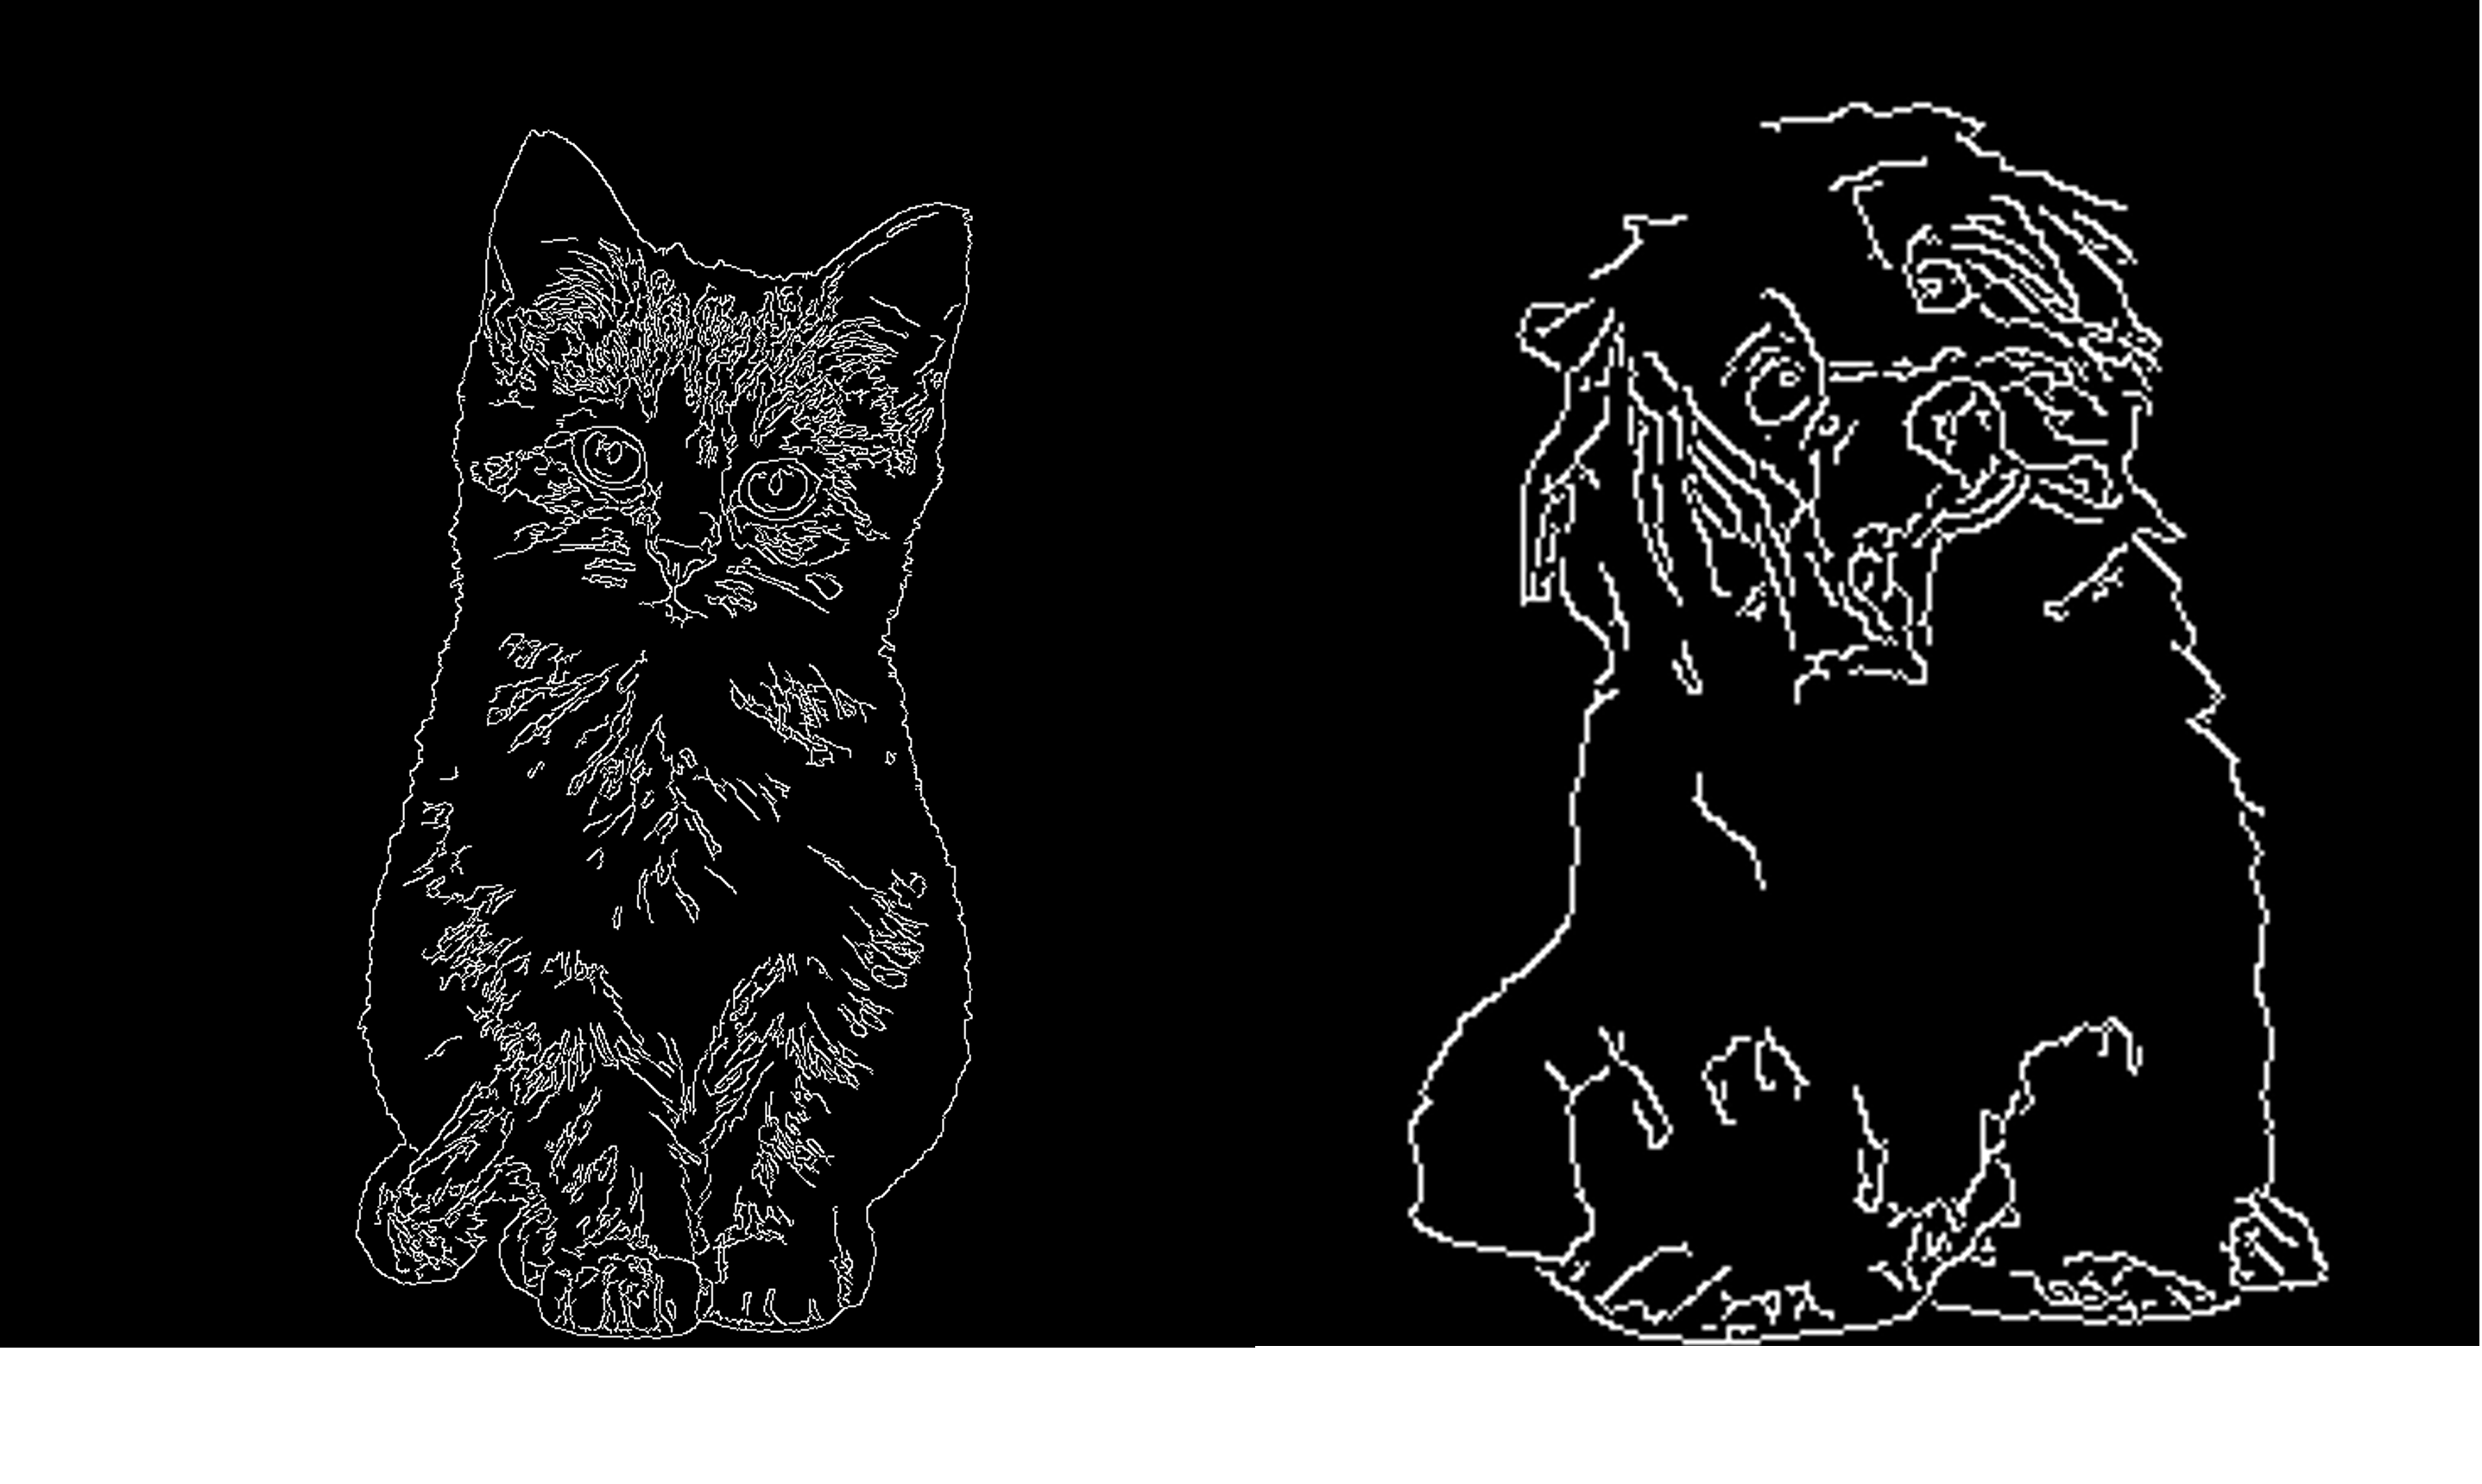
\includegraphics[width=\textwidth,height=\textheight,keepaspectratio]{figures/CatDog_edge.png}%
    % \includegraphics[width=0.475\textwidth]{Dog_edge.png}
\end{frame}
% \begin{frame}[fragile]{Intro to Machine Learning}
%     \textbf{Why Machine Learning?}
%     \href{https://www.youtube.com/playlist?list=PLe3zogoPd5DY07OpTP4nFNOdMqItwtgc2}{Videos}.
% \end{frame}
\begin{frame}[fragile]{Intro to Machine Learning}
    \textbf{Why Machine Learning?}
    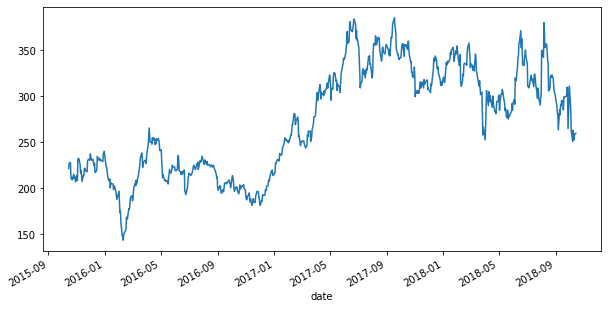
\includegraphics[width=\textwidth,height=\textheight,keepaspectratio]{figures/Stock_block.png}
\end{frame}
\begin{frame}[fragile]{Intro to Machine Learning}
    \textbf{Why Machine Learning?}
    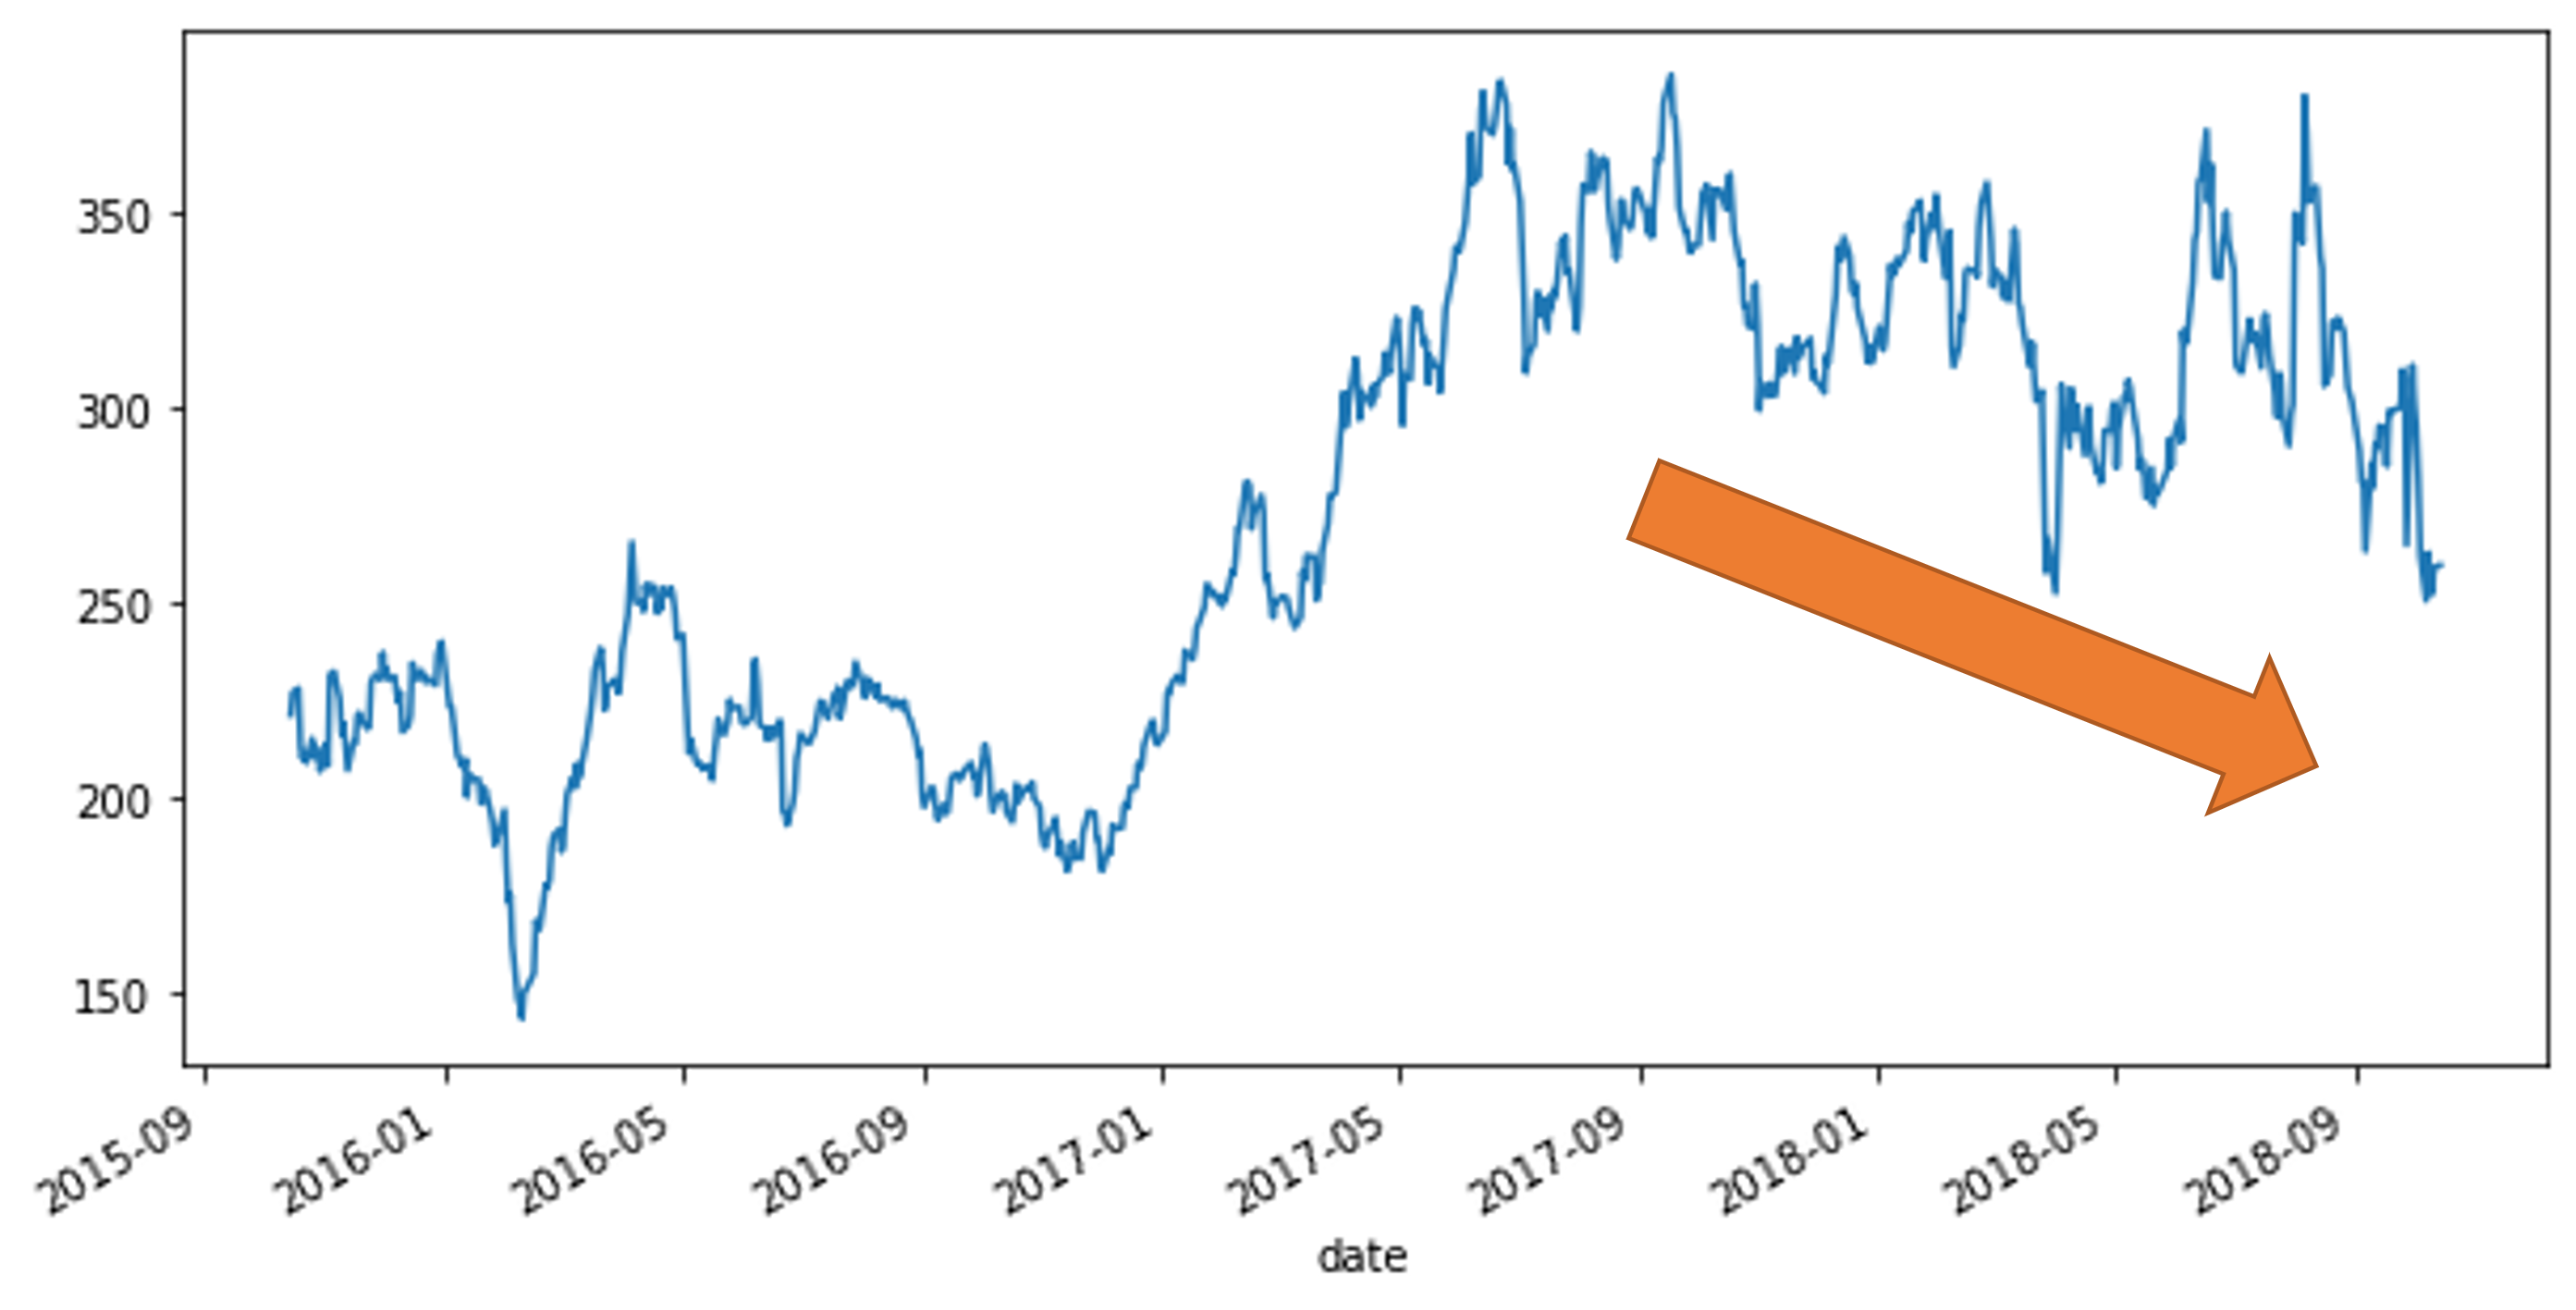
\includegraphics[width=\textwidth,height=\textheight,keepaspectratio]{figures/Stock_trend.png}
\end{frame}
\begin{frame}[fragile]{Intro to Machine Learning}
    \textbf{Why Machine Learning?}
    \begin{center}
        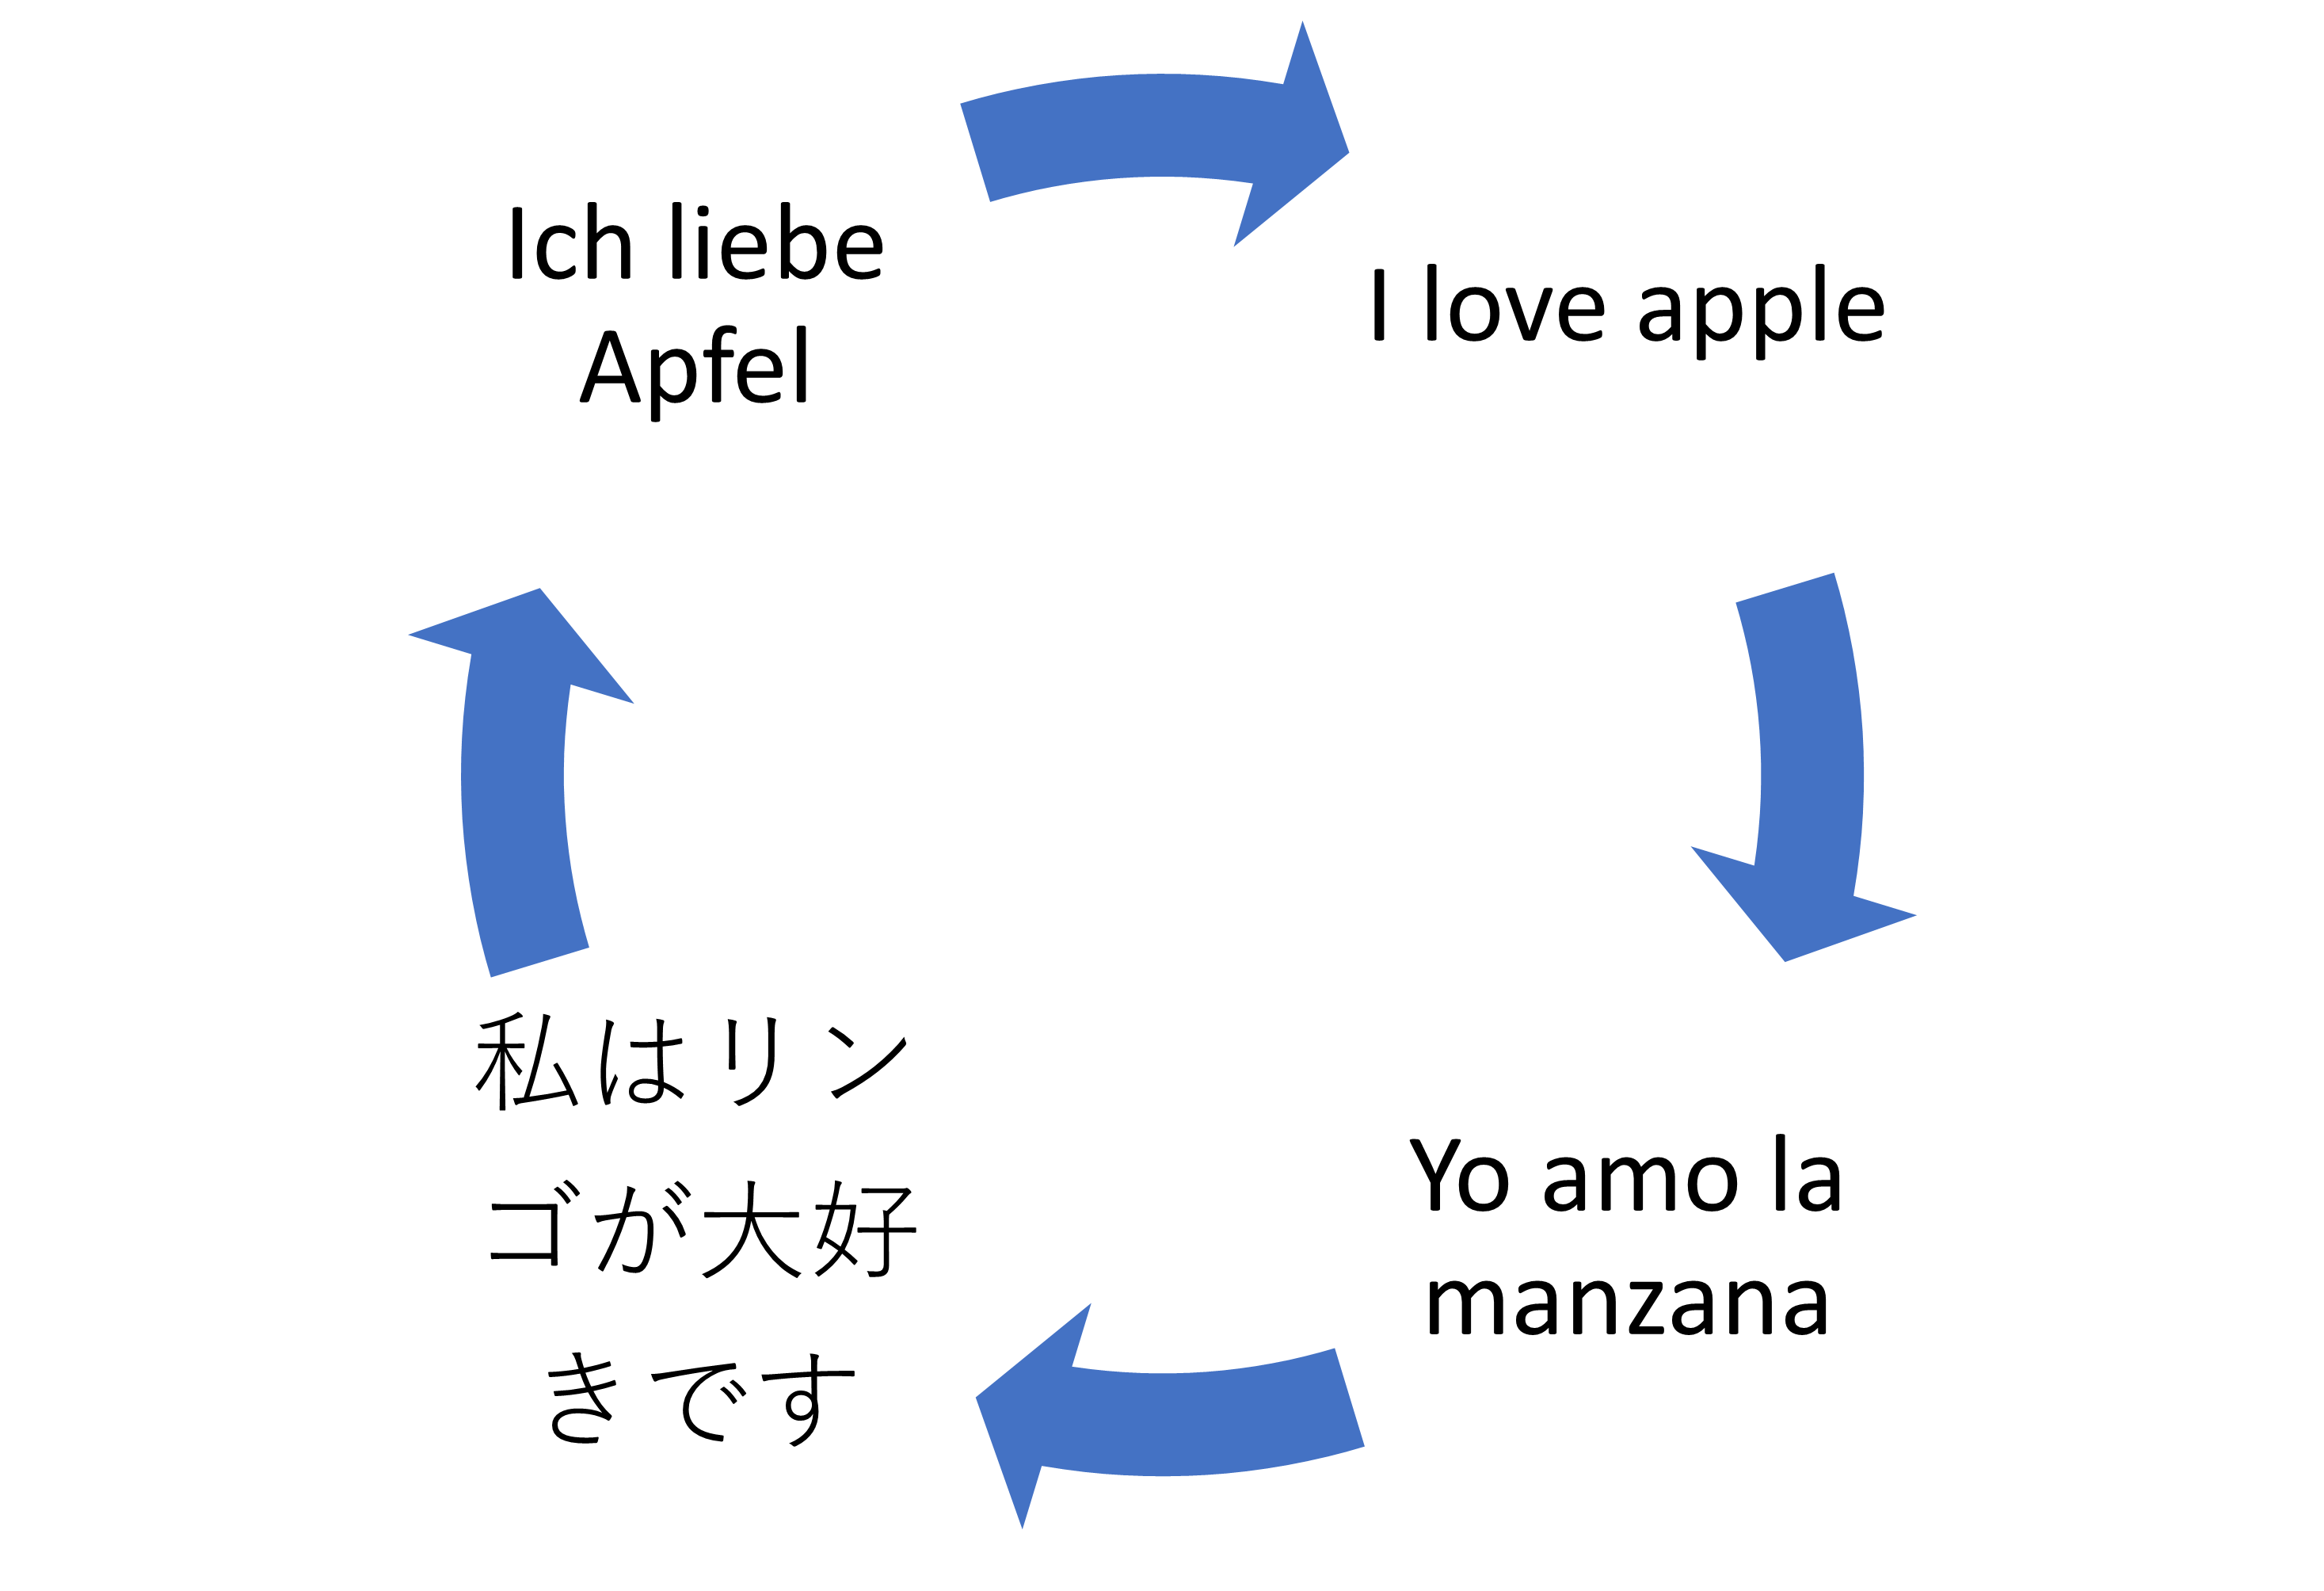
\includegraphics[width=\textwidth,height=0.8\textheight,keepaspectratio]{figures/Lang_1.png}
    \end{center}
\end{frame}
\begin{frame}[fragile]{Intro to Machine Learning}
    \textbf{Why Machine Learning?}
    \begin{center}
        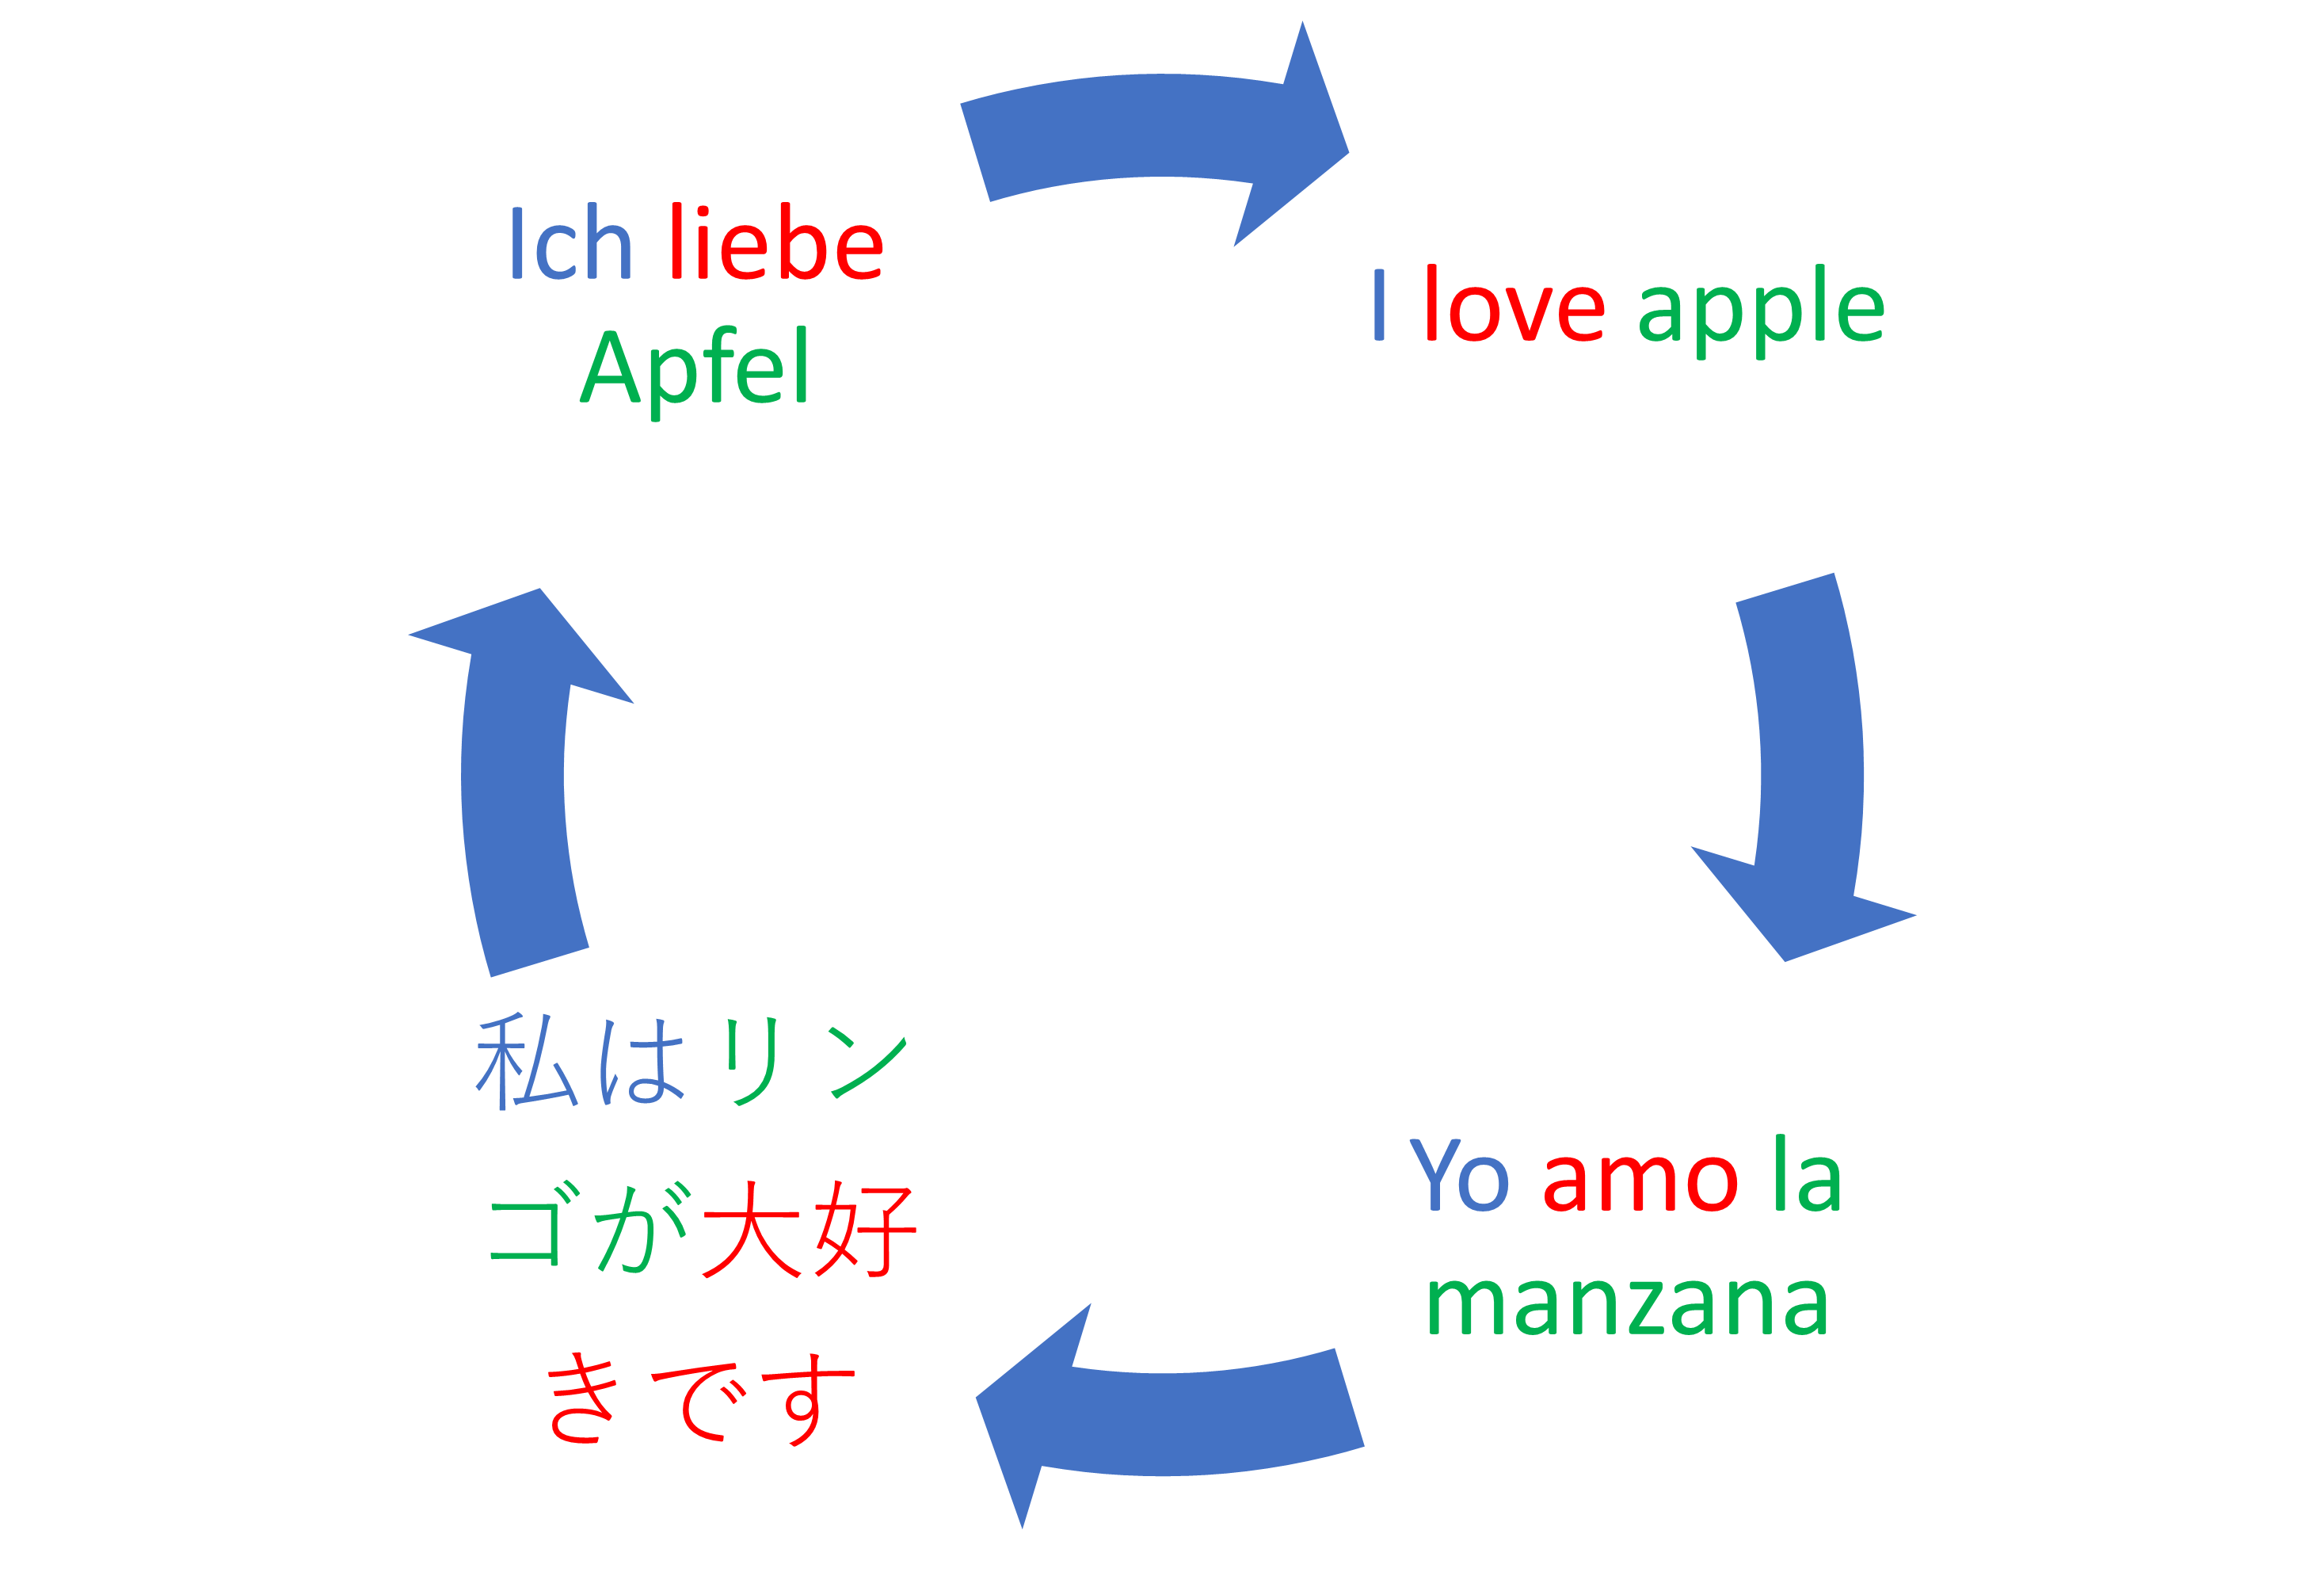
\includegraphics[width=\textwidth,height=0.8\textheight,keepaspectratio]{figures/Lang_2.png}
    \end{center}
\end{frame}

\begin{frame}[fragile]{Intro to Machine Learning}
    \begin{block}{What is Machine Learning?}
        \begin{itemize}
            \item A cross-discipline field of study that combines aspects of Data Science, Data Engineering, Statistics and Probabilities, and Computer Programming to model highly complex functions.
            \pause
            \item 90\% of the time is spent on cleaning and making the data work; 10\% of the time is spent on actual machine learning.
            \item \huge $f(x)$
        \end{itemize}
    \end{block}
\end{frame}
\begin{frame}[fragile]{Intro to Machine Learning}
    \textbf{What is Machine Learning?}
    \begin{block}{Artificial Intelligence}
        \textbf{Artificial Intelligence} is a question: How do we build systems that solve tasks for which humans need intelligence?
    \end{block}
    \begin{block}{Machine Learning}
        \textbf{Machine Learning} is the contemporary answer to the question: a set of techniques/algorithms that allow computers to learn to solve tasks from data.
    \end{block}
\end{frame}

\begin{frame}[fragile]{Intro to Machine Learning}
    \textbf{Types of Machine Learning task}
    \begin{itemize}
        \item Supervised Learning
        \item Unsupervised Learning
        \item Reinforcement Learning
    \end{itemize}
\end{frame}

\begin{frame}[fragile]{Intro to Machine Learning}
    \textbf{Supervised Learning}
    \begin{center}
        
\includegraphics[width=\textwidth,height=0.7\textheight,keepaspectratio]{figures/Target.png}
    \end{center}
\end{frame}
\begin{frame}[fragile]{Intro to Machine Learning}
    \textbf{Supervised Learning}
    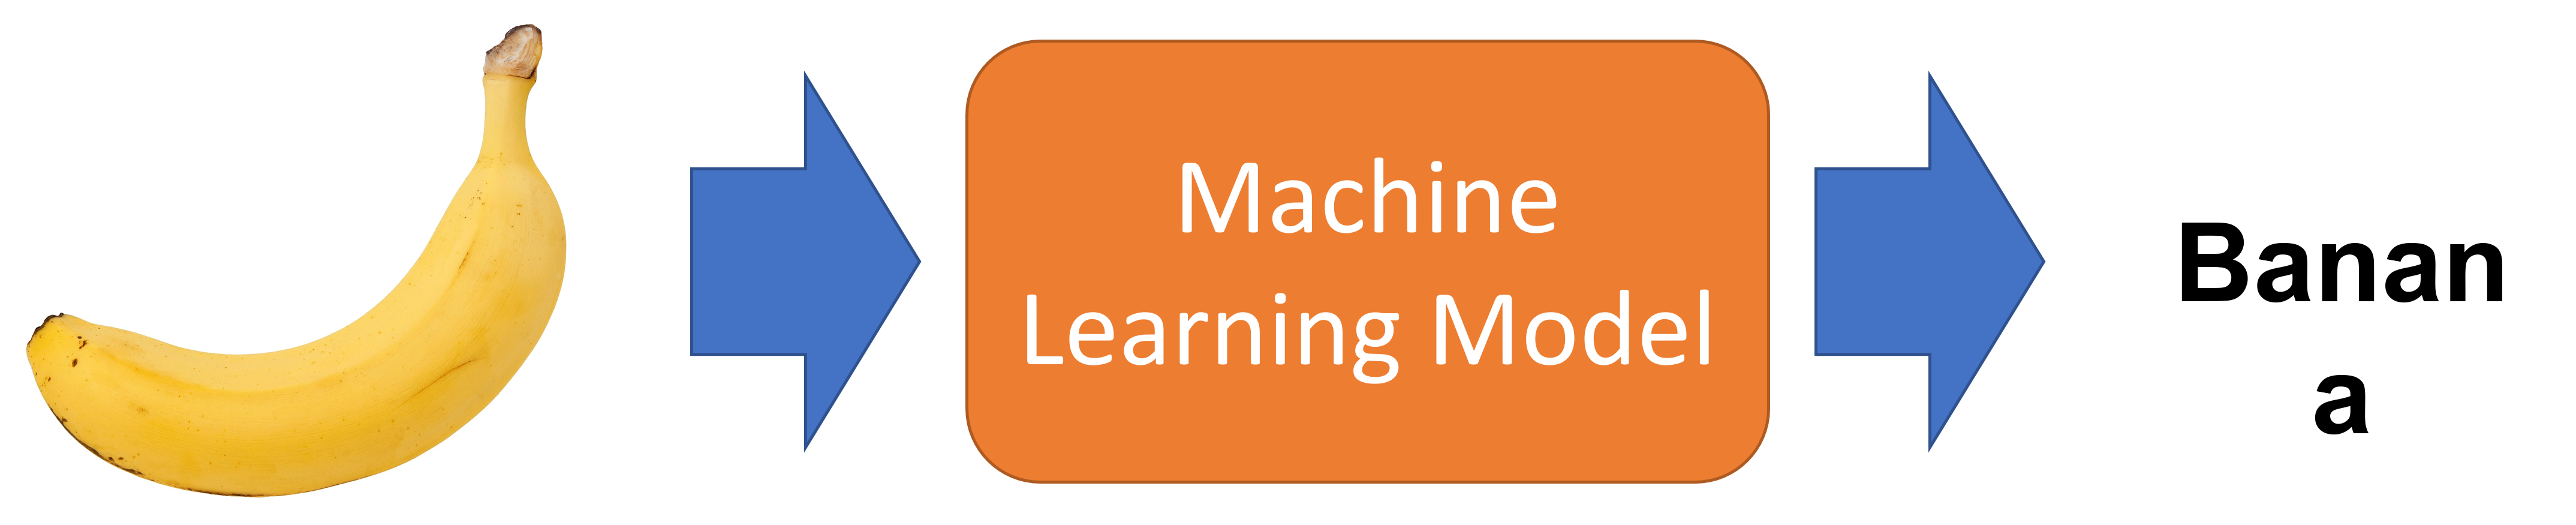
\includegraphics[width=\textwidth,height=\textheight,keepaspectratio]{figures/Supervised_example_1.png}
\end{frame}
\begin{frame}[fragile]{Intro to Machine Learning}
    \textbf{Supervised Learning}
    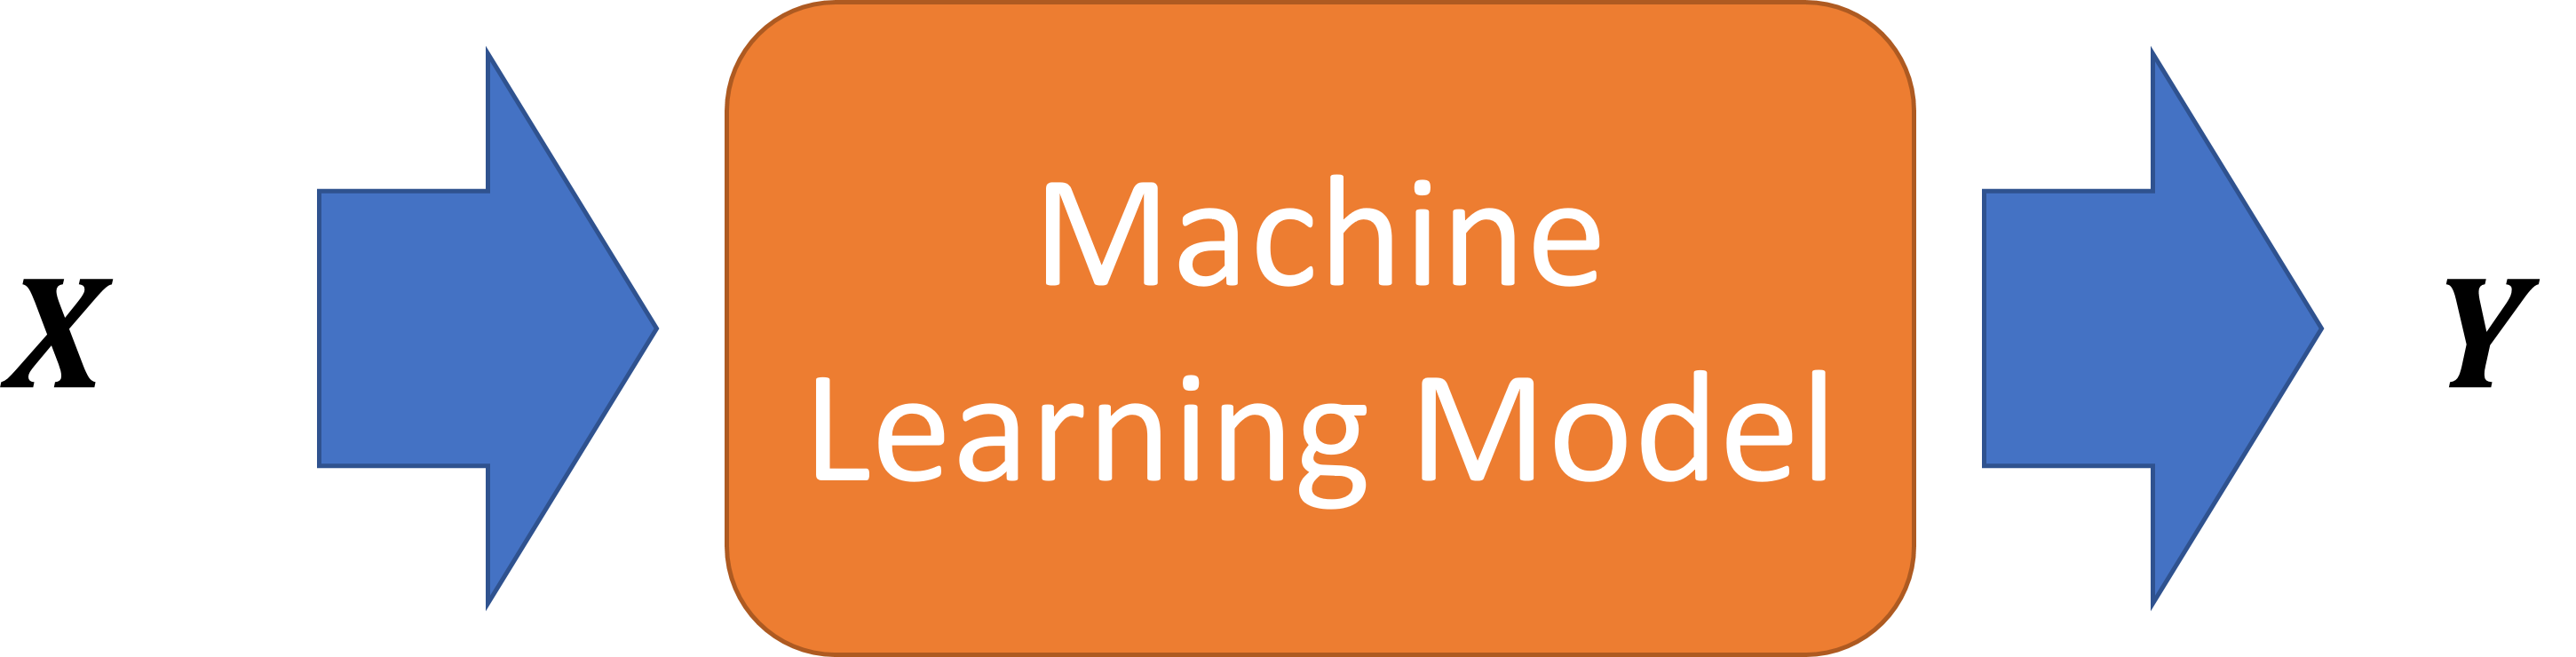
\includegraphics[width=\textwidth,height=\textheight,keepaspectratio]{figures/Supervised.png}
\end{frame}
\begin{frame}[fragile]{Intro to Machine Learning}
    \textbf{Supervised Learning}
    \begin{itemize}
        \item is a machine learning paradigm that learns a mapping function between input and output data.
        \item needs pairs of input features and labelled output targets.
        \pause
        \item sensitive to target's noise and outliers.
        \item has a bias-variance dilemma.
        \item affected by the curse of dimensionality and complexity.
    \end{itemize}
\end{frame}

\begin{frame}[fragile]{Intro to Machine Learning}
    \textbf{Unsupervised Learning}
    \begin{center}
        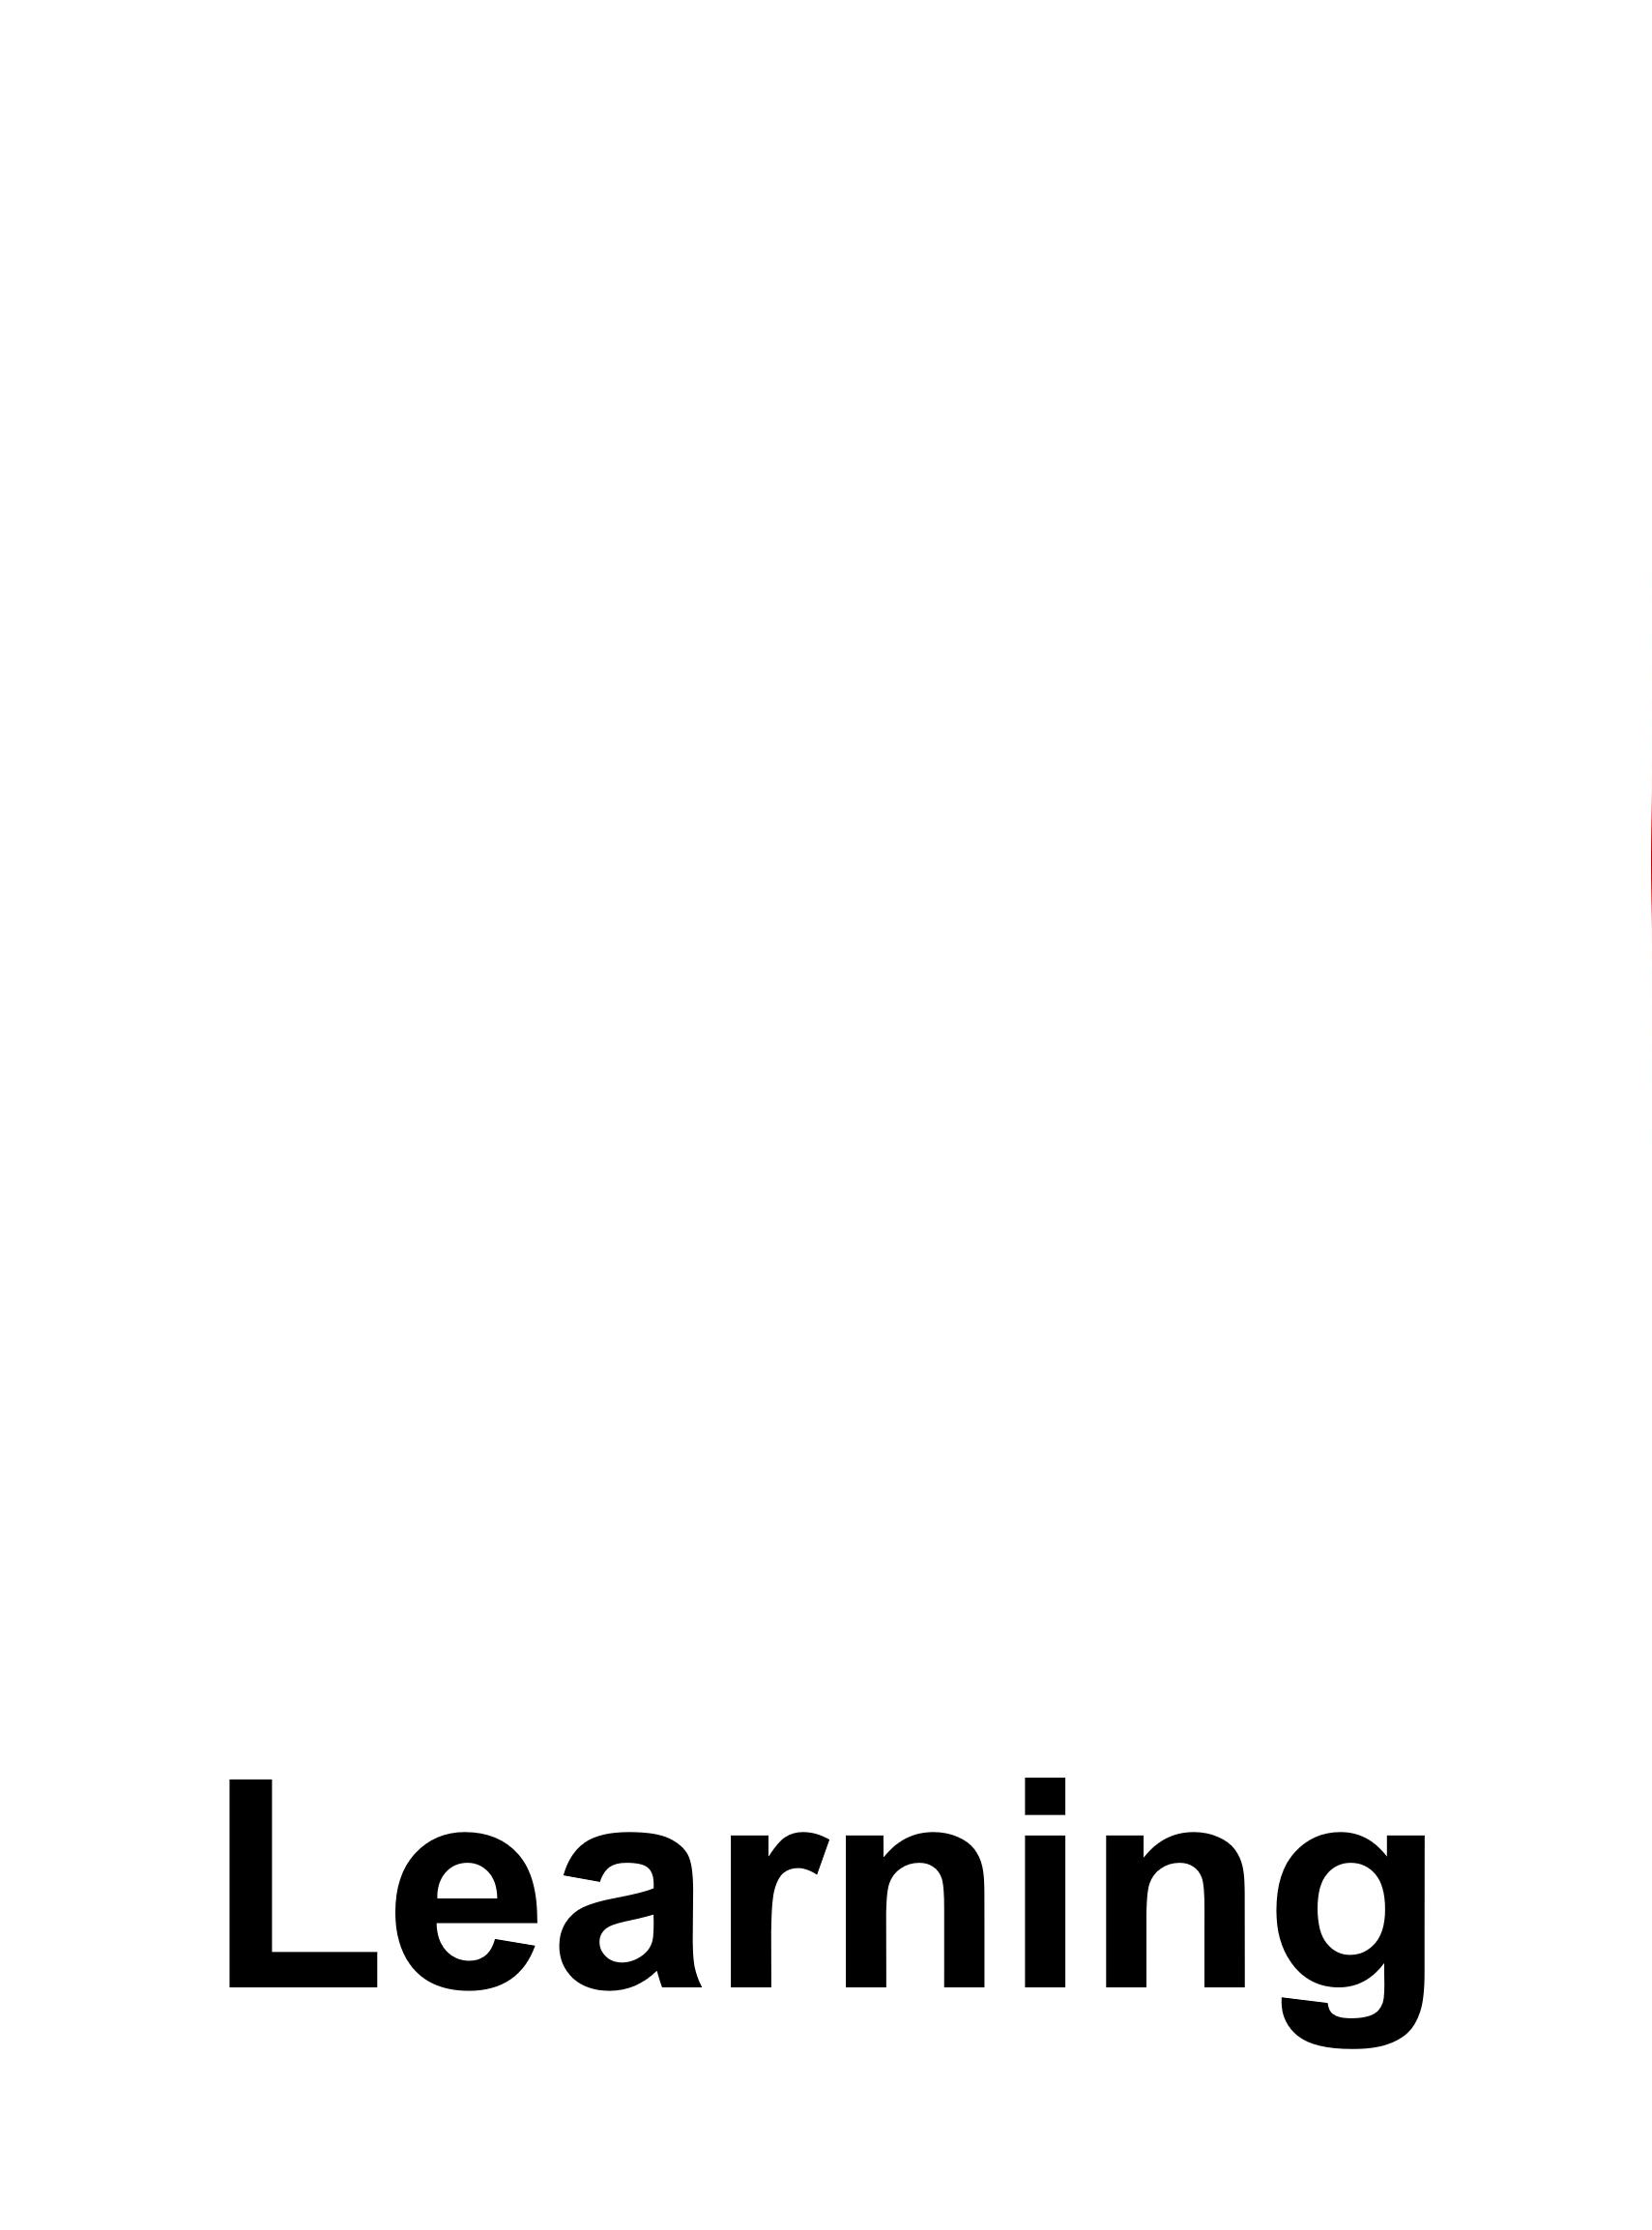
\includegraphics[width=\textwidth,height=0.7\textheight,keepaspectratio]{figures/UnTarget.png}
    \end{center}
\end{frame}
\begin{frame}[fragile]{Intro to Machine Learning}
    \textbf{Unsupervised Learning}
    \includegraphics[width=\textwidth,height=\textheight,keepaspectratio]{figures/Unsupervised_example.png}
\end{frame}
\begin{frame}[fragile]{Intro to Machine Learning}
    \textbf{Unsupervised Learning}
    \begin{center}
        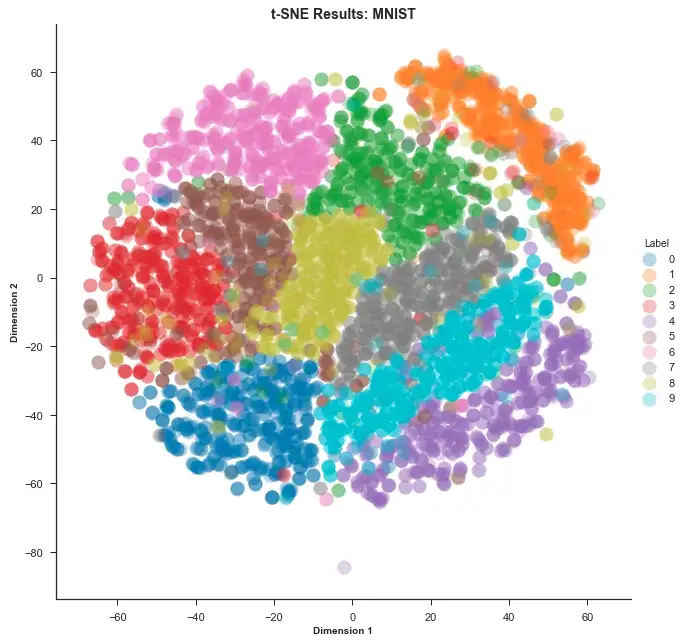
\includegraphics[width=\textwidth,height=0.7\textheight,keepaspectratio]{figures/tSNE.png}
    \end{center}
\end{frame}
\begin{frame}[fragile]{Intro to Machine Learning}
    \textbf{Unsupervised Learning}
    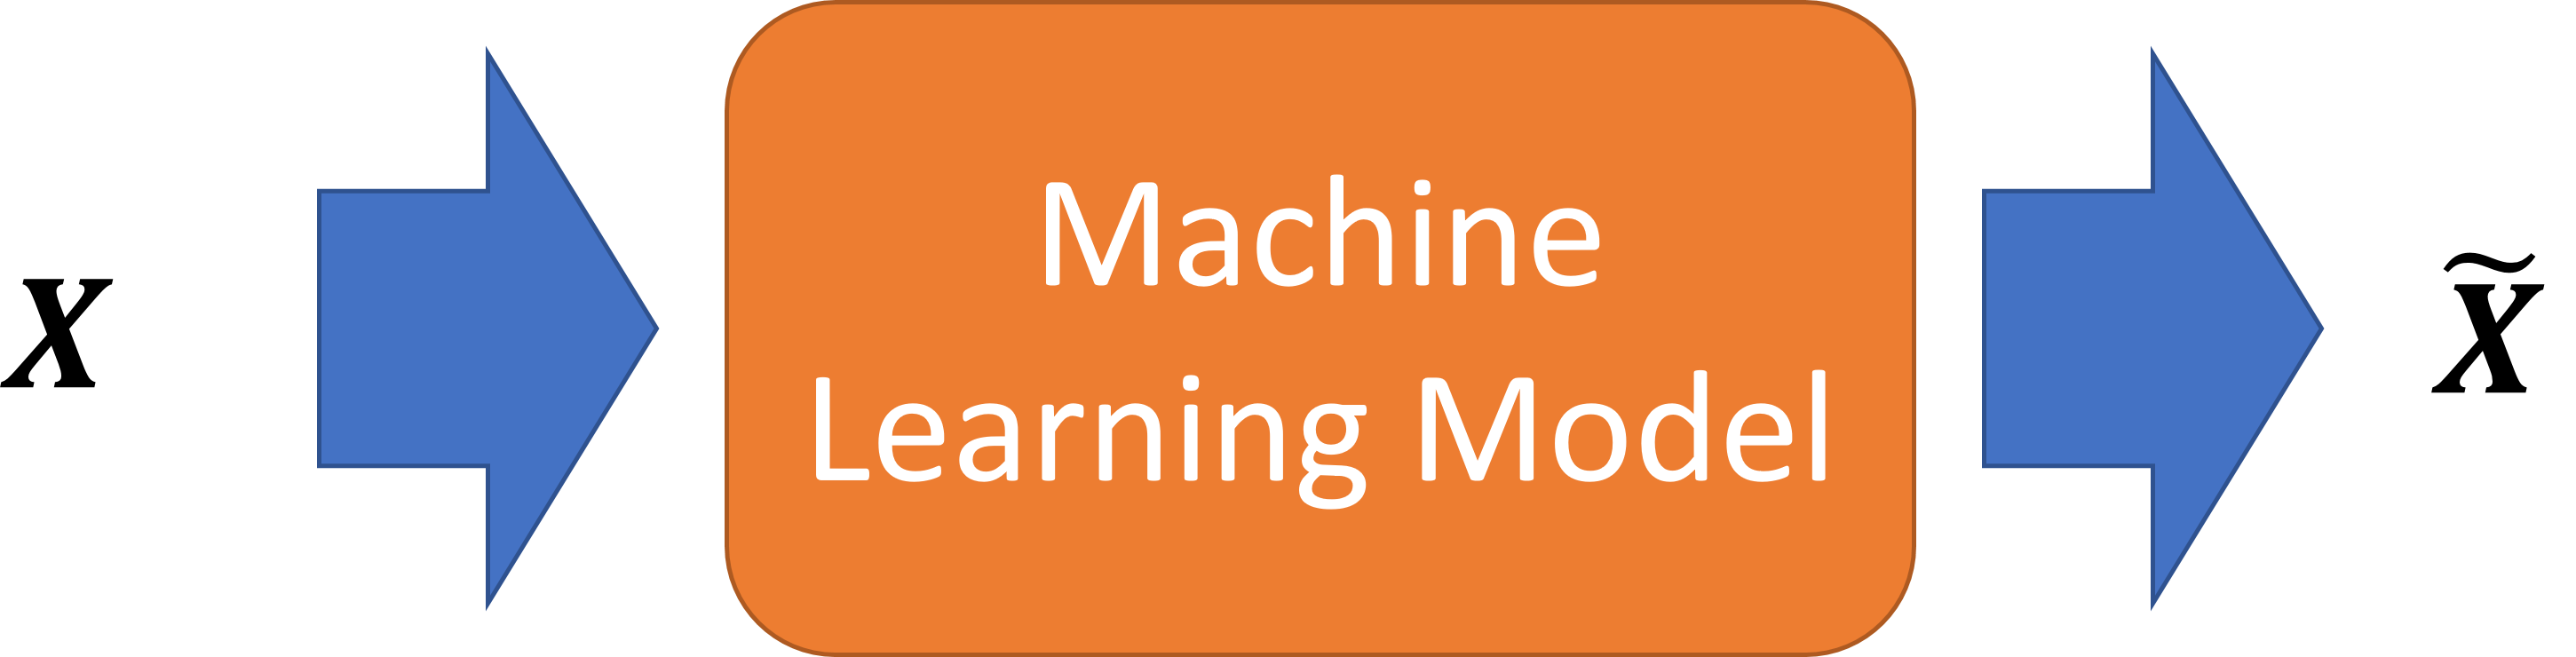
\includegraphics[width=\textwidth,height=\textheight,keepaspectratio]{figures/Unsupervised.png}
\end{frame}
\begin{frame}[fragile]{Intro to Machine Learning}
    \textbf{Unsupervised Learning}
    \begin{itemize}
        \item is a machine learning paradigm that learns underlying patterns from input data.
        \item usually performs clustering and dimensional reduction.
        \pause
        \item sensitive to input's noise and outliers.
        \item has a bias-variance dilemma.
        \item Less accurate than supervised learning.
    \end{itemize}
\end{frame}

\begin{frame}[fragile]{Intro to Machine Learning}
    \textbf{Reinforcement Learning}
    \begin{center}
        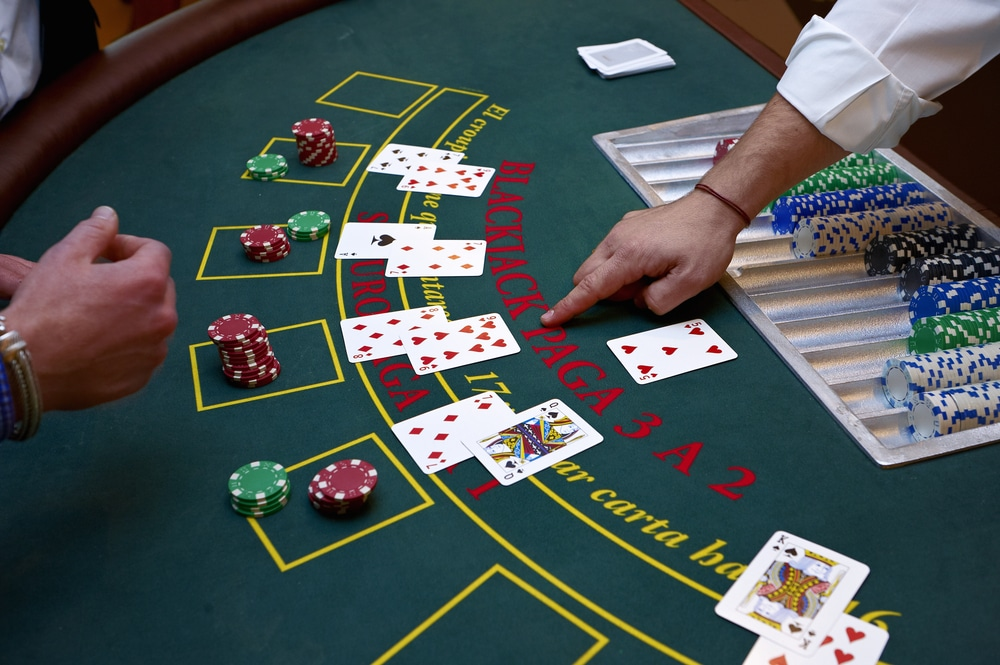
\includegraphics[width=\textwidth,height=0.7\textheight,keepaspectratio]{figures/Blackjack.jpg}
    \end{center}
\end{frame}
\begin{frame}[fragile]{Intro to Machine Learning}
    \textbf{Reinforcement Learning}
    \begin{center}
        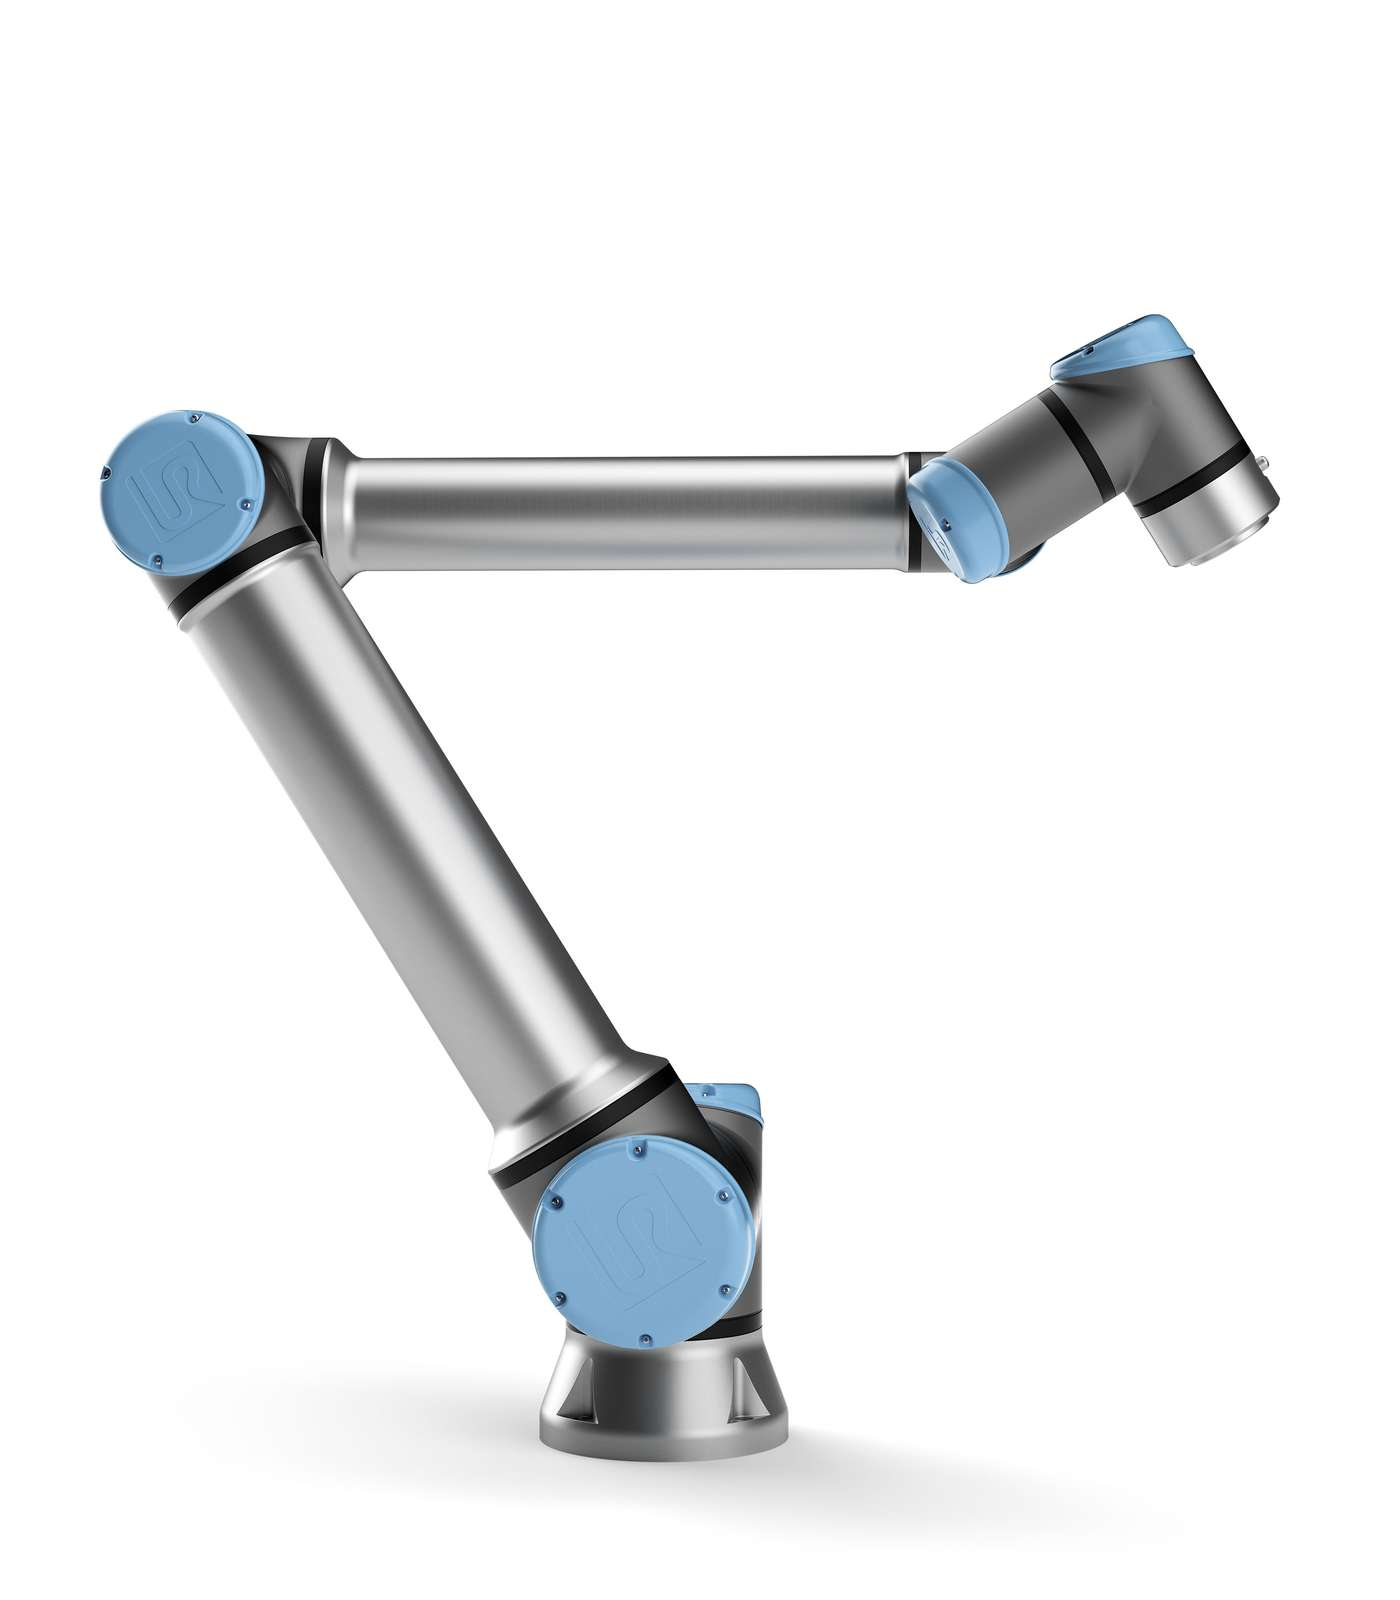
\includegraphics[width=\textwidth,height=0.7\textheight,keepaspectratio]{figures/UR10e.jpg}
    \end{center}
\end{frame}
\begin{frame}[fragile]{Intro to Machine Learning}
    \textbf{Reinforcement Learning}
    \begin{center}
        \includegraphics[width=\textwidth,height=\textheight,keepaspectratio]{figures/High-Jump.png}
    \end{center}
\end{frame}
\begin{frame}[fragile]{Intro to Machine Learning}
    \textbf{Reinforcement Learning}
    \begin{center}
        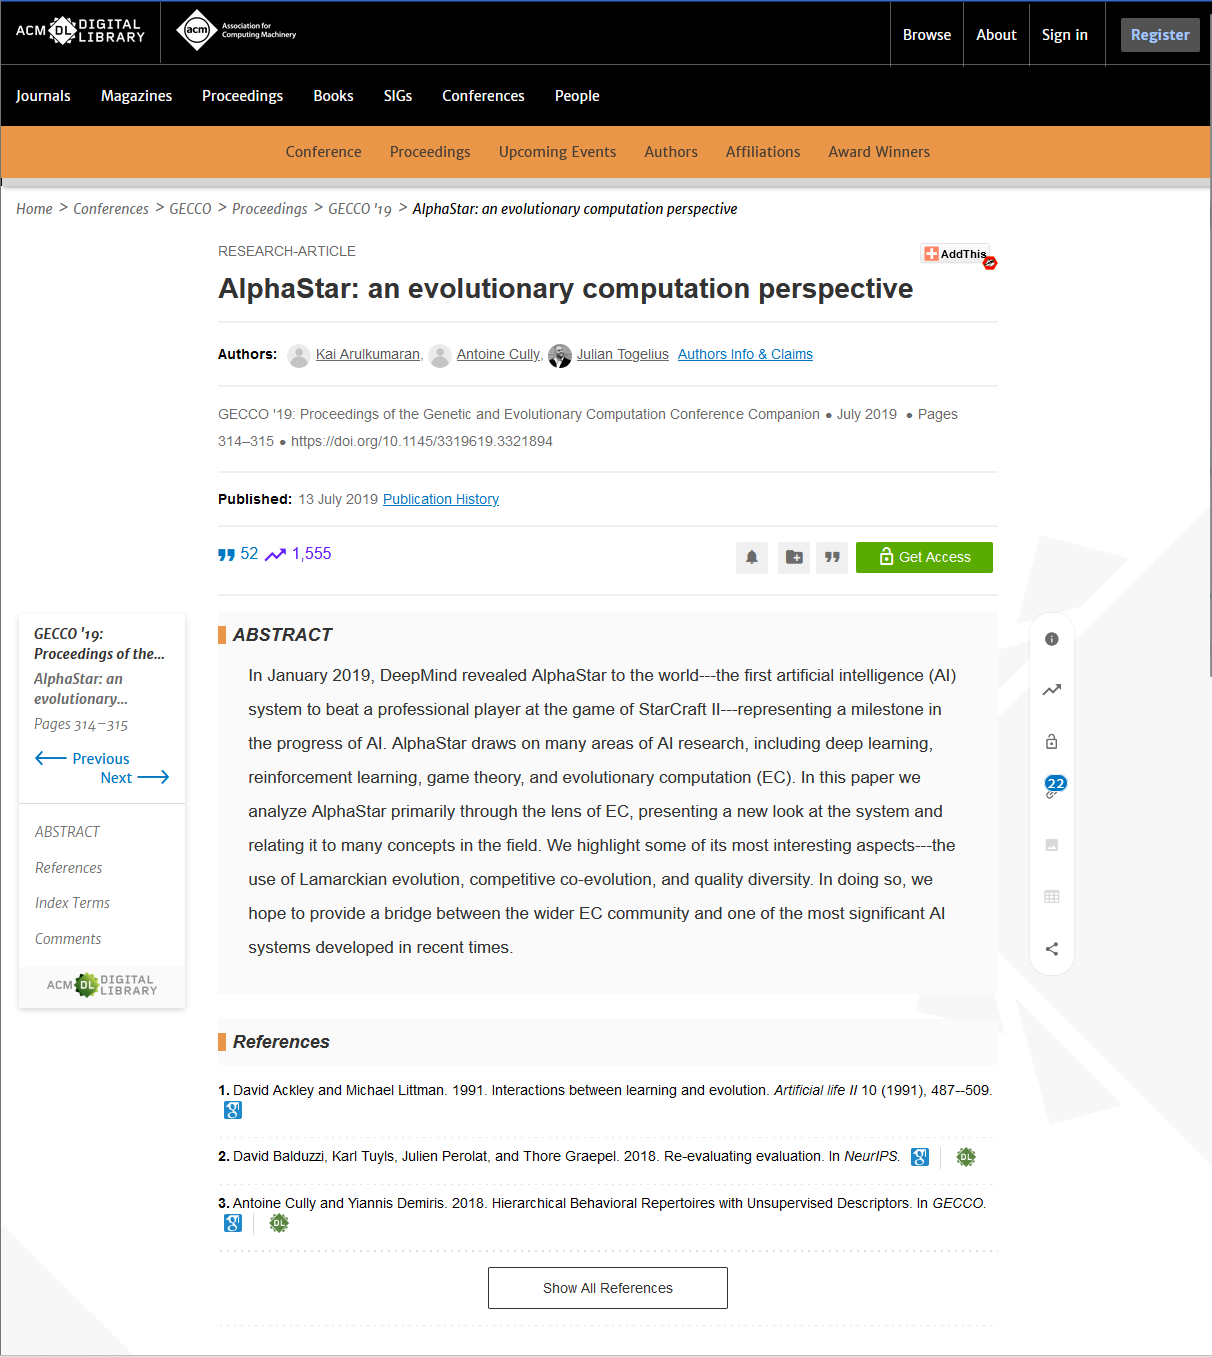
\includegraphics[width=\textwidth,height=0.7\textheight,keepaspectratio]{figures/AlphaStar.png}
    \end{center}
\end{frame}
\begin{frame}[fragile]{Intro to Machine Learning}
    \textbf{Reinforcement Learning}
    \begin{center}
        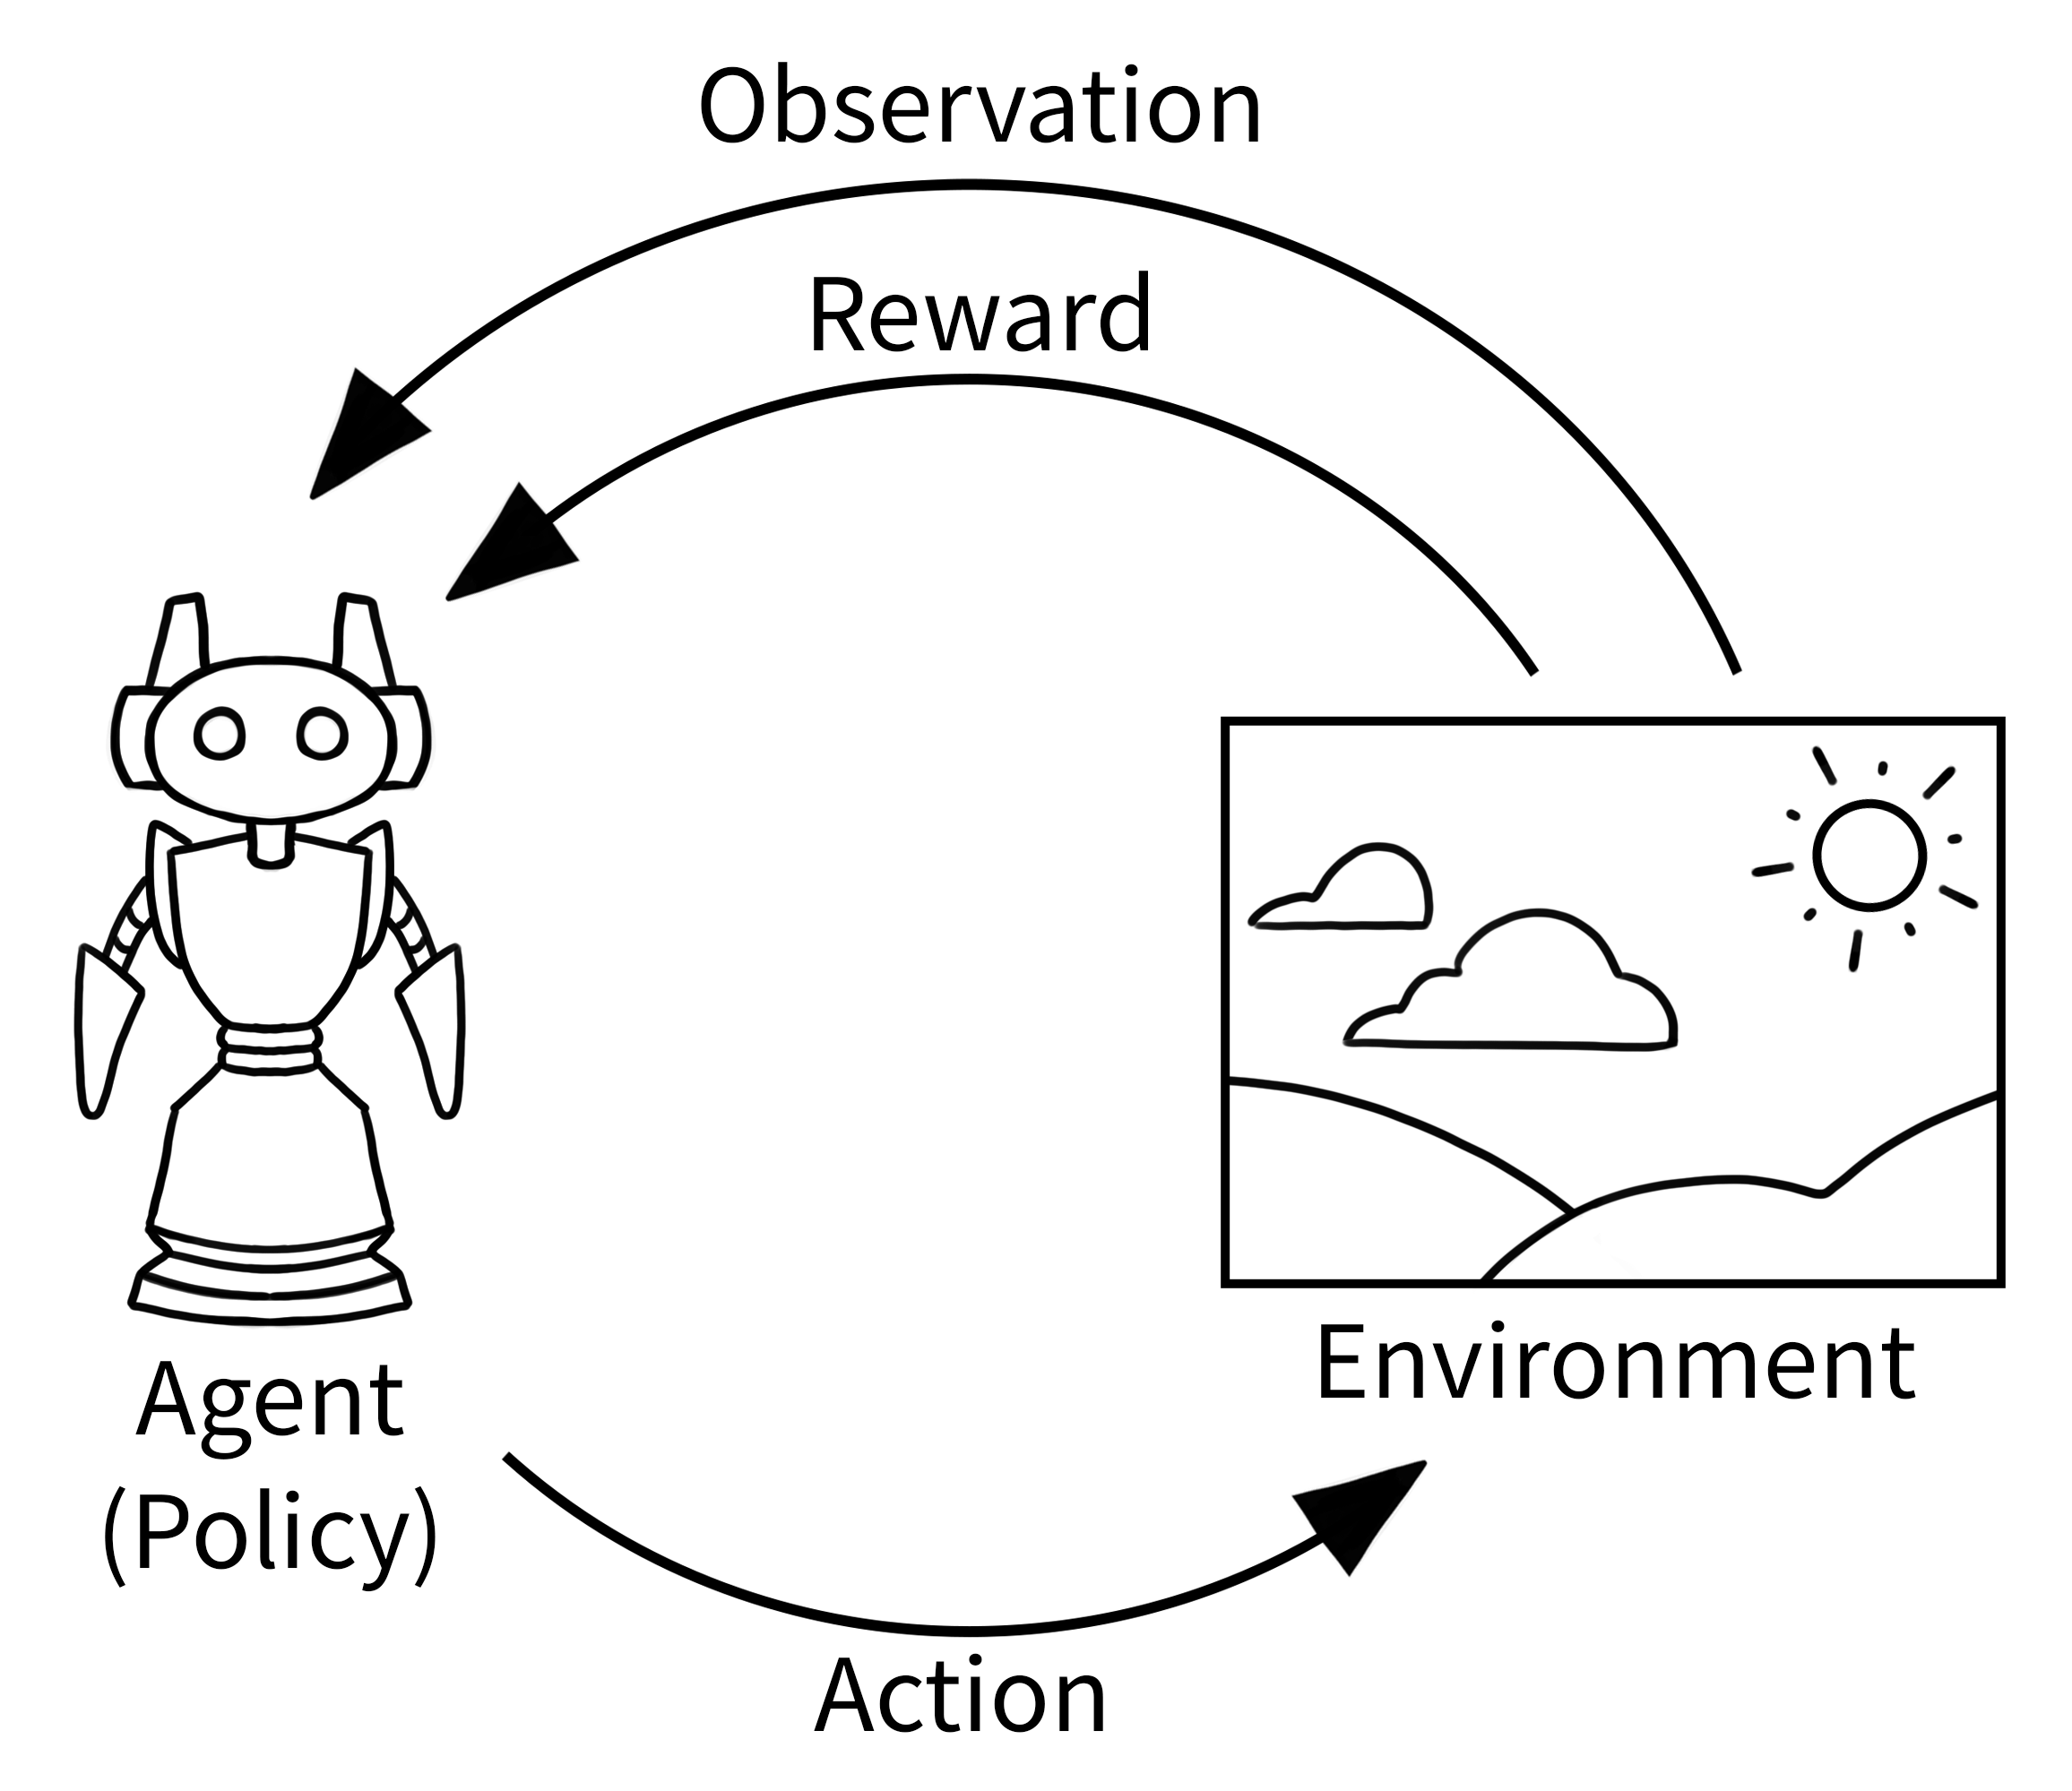
\includegraphics[width=\textwidth,height=0.6\textheight,keepaspectratio]{figures/RL.png}
    \end{center}
\end{frame}
\begin{frame}[fragile]{Intro to Machine Learning}
    \textbf{Reinforcement Learning}
    \begin{itemize}
        \item is a machine learning system that learns to perform a task by interacting with its environment.
        \item has no supervisor signal.
        \item has delayed feedback.
        \item agent's actions affect future environments and the subsequent data.
        \item allows the agent to learn an optimal policy that maximizes long-term rewards.
    \end{itemize}
\end{frame}
\begin{frame}[fragile]{Intro to Machine Learning}
    \begin{center}
        \Huge Types of Machine Learning models
    \end{center}            
\end{frame}

\begin{frame}[fragile]{Intro to Machine Learning}
    \textbf{Types of Machine Learning models}\\
    \begin{itemize}
        \item By Model
        \item By Data
    \end{itemize}
\end{frame}

\begin{frame}[fragile]{Intro to Machine Learning}
    \textbf{By Model}\\
    ML models are categorised by how the model information is stored.
    \begin{itemize}
        \item Non-parametric models: All information, including training data, is stored within the model.
        \item Parametric models: Parametric models: Models store parameterised information derived from training data, including any specific parameter settings
    \end{itemize}
\end{frame}

\begin{frame}[fragile]{Intro to Machine Learning}
    \textbf{By Data}\\
    ML models are organised by the type of Data they interact with.
    \begin{center}
        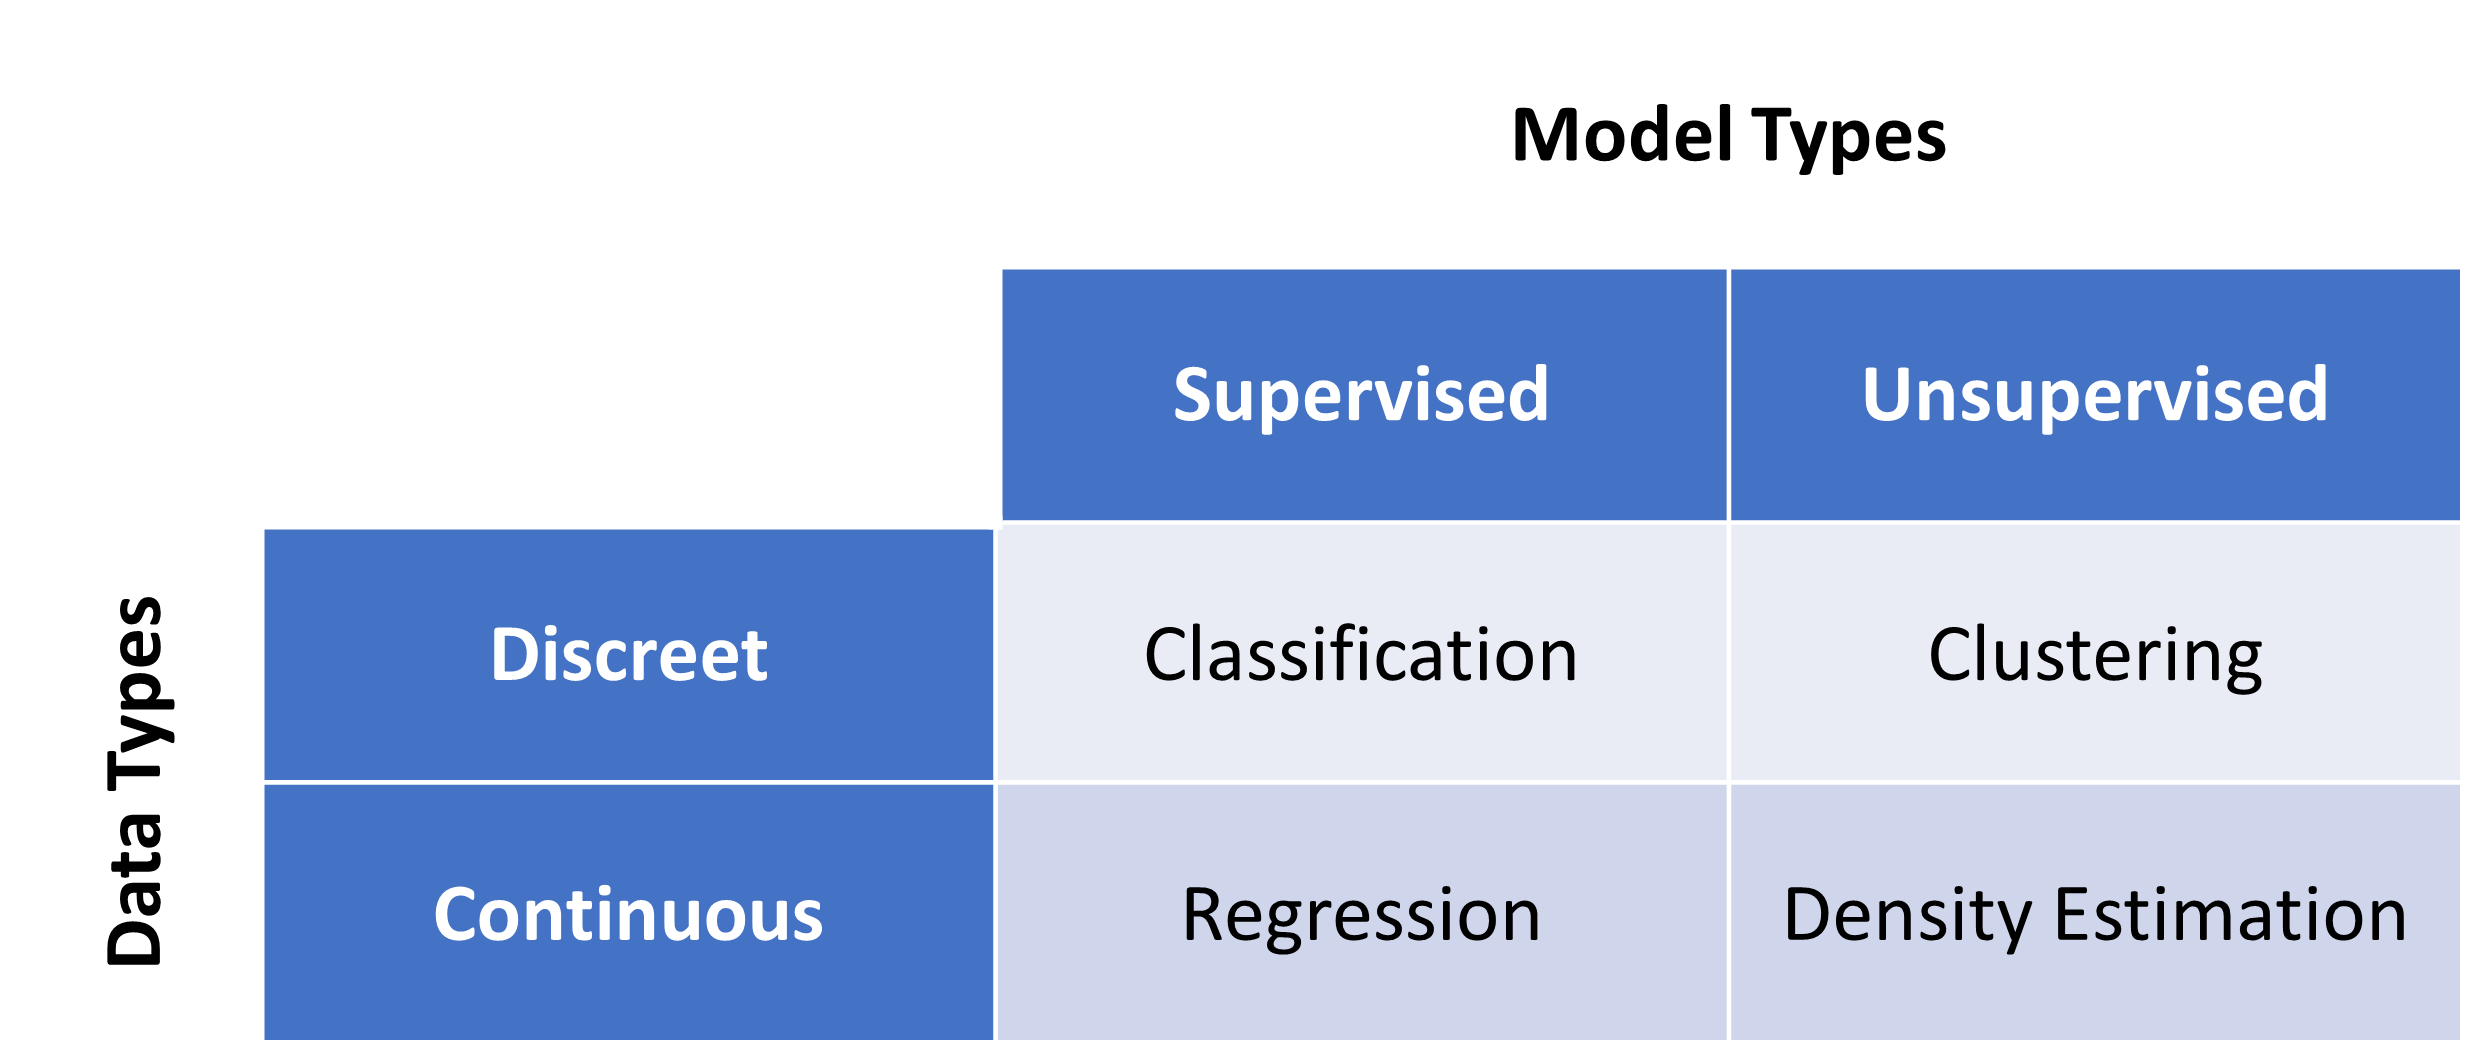
\includegraphics[width=\textwidth,height=\textheight,keepaspectratio]{figures/By-Data.png}
    \end{center}
\end{frame}

\begin{frame}[fragile]{Types of Machine Learning}
    Generally, the domain of Machine Learning can be divided into two fields:
    \begin{itemize}
        \item Classical Machine Learning, where models rely on prior domain knowledge and hand-crafted features to function correctly.
        \item Contemporary Machine (Deep) Learning, where prior domain knowledge is optional, and models typically rely on feature extraction layers and deeper depth to function.
    \end{itemize}
\end{frame}
% 2 weeks
\subsection{Classical Machine Learning}
\begin{frame}[fragile]{Classical Machine Learning}
    \vspace{-0.5cm}
    \textbf{Linear Models}
    \begin{block}{Definition}
        A model that describes the relationship between observations, $Y$, and input samples, $(X_1, X_2,..., X_p)$, as a weighted linear combination. Linear models assume that each input sample, $X_i$, is independent.
    \end{block}
    \vspace{-1cm}
    \begin{equation}
        y_i = w_0 + w_1 x_1 + w_2 x_2 + ... + w_p x_p
    \end{equation}
    Where $y_i$ is the $i$-th observation, $x_i$ is the $i$-th input sample, and $w_i$ is the weight.
    However, linear models are usually expressed in a full matrix form:
    \begin{equation}
        \label{eq:2}
        Y = XW^T + \epsilon
    \end{equation}
    where $Y$ is the matrix of observations, $X$ is the matrix of input samples, $W$ is the matrix of weights, and $\epsilon$ is the error term.
\end{frame}
\begin{frame}[fragile]{Classical Machine Learning}
    \textbf{Linear Regression}
    \href{https://scikit-learn.org/stable/modules/generated/sklearn.linear_model.LinearRegression.html}{\textbf{\underline{sklearn.linear\_model.LinearRegression}}}
    \begin{example}
        \begin{lstlisting}[language=Python]
from sklearn.linear_model import LinearRegression

reg = LinearRegression() # Initialise model
reg.fit(samples, targets) # Fit model to data
reg.predict(test_samples) # Make prediction
reg.score(test_samples, test_targets) # Evaluate
        \end{lstlisting}
    \end{example}
\end{frame}
\begin{frame}[fragile]{Classical Machine Learning}
    \textbf{Logistic Regression}
    \begin{block}{Definition}
        Logistic Regression is a discretized version of a linear regression model. To discretize the output, Logistic Regression uses sigmoid or softmax to map arbitrary numbers $\in \mathbb{R}$ to the [0, 1] range.
        \begin{columns}[T]
            \begin{column}{.40\textwidth}
                \begin{center}
                    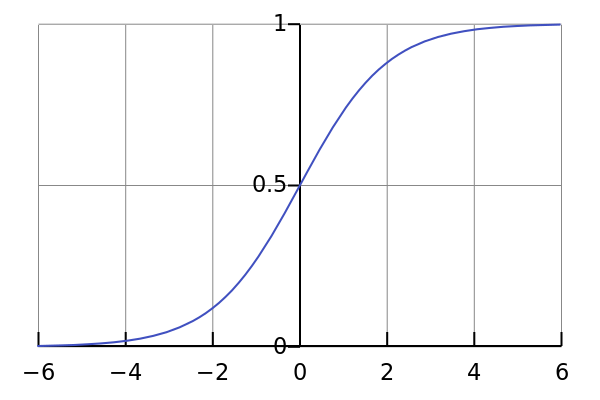
\includegraphics[width=.80\textwidth,height=\textheight,keepaspectratio]{figures/Logistic-Sigmoid.png}
                \end{center}
            \end{column}%
            \hfill%
            \begin{column}{.40\textwidth}
                Sigmoid function:
                \begin{equation*}
                    \sigma(x) = \frac{1}{1 + \exp^{-x}}
                \end{equation*}
                Softmax function:
                \begin{equation*}
                    softmax(x)_{i} = \frac{\exp^{x_{i}}}{\sum_{j=1}^{K}\exp^{x_{j}}}
                \end{equation*}
            \end{column}%
        \end{columns}
    \end{block}
\end{frame}
\begin{frame}[fragile]{Classical Machine Learning}
    \textbf{Logistic Regression}
    \href{https://scikit-learn.org/stable/modules/generated/sklearn.linear_model.LogisticRegression.html}{\textbf{\underline{sklearn.linear\_model.LogisticRegression}}}
    \begin{example}
        \begin{lstlisting}[language=Python]
from sklearn.linear_model import LogisticRegression

clf = LogisticRegression(random_state=0) # Initialise model
clf.fit(samples, targets) # Fit model to data
clf.predict(test_samples) # Make prediction
clf.score(test_samples, test_targets) # Evaluate
        \end{lstlisting}
    \end{example}
\end{frame}
\begin{frame}[fragile]{Classical Machine Learning}
    \textbf{K-Mean clustering}
    \begin{block}{Definition}
        K-Mean is a clustering algorithm that tries to divide a set of $N$ samples into $K$ disjointed clusters of equal variance, each with centroid, $\mu_{i}$. To cluster the data, K-Mean places centroids at places that minimize:
        \vspace{-0.5cm}
        \begin{equation*}
            L(Cluster) = \sum_{i=0}^{n}\min\limits_{\mu_{j}\in C}(||x_{i} - \mu_{j}||^2)
        \end{equation*}
        where $C$ is the set of clusters.
        \begin{center}
            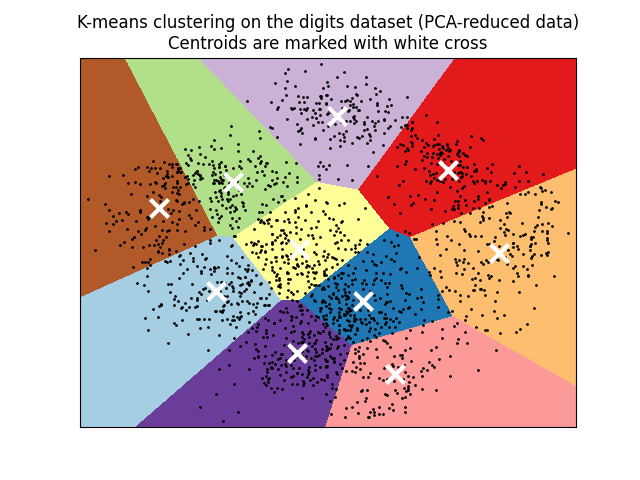
\includegraphics[width=.30\textwidth,height=\textheight,keepaspectratio]{figures/k_mean.png}
        \end{center}
    \end{block}
\end{frame}
\begin{frame}[fragile]{Classical Machine Learning}
    \textbf{K-Mean clustering}
    \href{https://scikit-learn.org/stable/modules/generated/sklearn.cluster.KMeans.html}{\textbf{\underline{sklearn.cluster.KMeans}}}
    \begin{example}
        \begin{lstlisting}[language=Python]
from sklearn.cluster import KMeans

kmeans = KMeans(n_clusters=2, random_state=0, n_init="auto")
kmeans.fit(samples) # Fit model to data
kmeans.predict(test_samples) # Make prediction
        \end{lstlisting}
    \end{example}
\end{frame}

\begin{frame}[fragile]{Classical Machine Learning}
    \textbf{Principal component analysis}
    Similar to K-Mean, PCA is an unsupervised algorithm. However, unlike K-Mean, PCA operates on continuous variables to conduct dimensionality reduction. The principle of PCA is to decompose multivariate variables into a set of successive orthogonal components with a maximum amount of variance in each direction.
    \begin{center}
        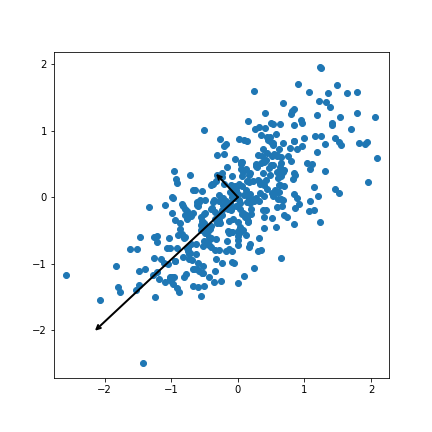
\includegraphics[width=.40\textwidth,height=\textheight,keepaspectratio]{figures/PCA.png}
    \end{center}
\end{frame}
\begin{frame}[fragile]{Classical Machine Learning}
    \textbf{Principal component analysis}
    \href{https://scikit-learn.org/stable/modules/generated/sklearn.decomposition.PCA.html}{\textbf{\underline{sklearn.decomposition.PCA}}}
    \begin{example}
        \begin{lstlisting}[language=Python]
from sklearn.decomposition import PCA

pca = PCA(n_components=2)
pca.fit(samples) # Fit model to data
pca.transform(test_samples) # Decompose data
        \end{lstlisting}
    \end{example}
\end{frame}
\begin{frame}[fragile]{Classical Machine Learning}
    \textbf{Train-Test Split}
    One of the most common pitfalls in early-stage Machine Learning is training and evaluating the model on the same dataset, as the model would repeat previously seen connections between input samples and targeted observations, commonly known as overfitting. To truly assess the model's generalizability, the model must be evaluated on an unseen dataset, preferably in an adjacent distribution. To avoid overfitting, the dataset is usually split into training and testing sets.
    \begin{center}
        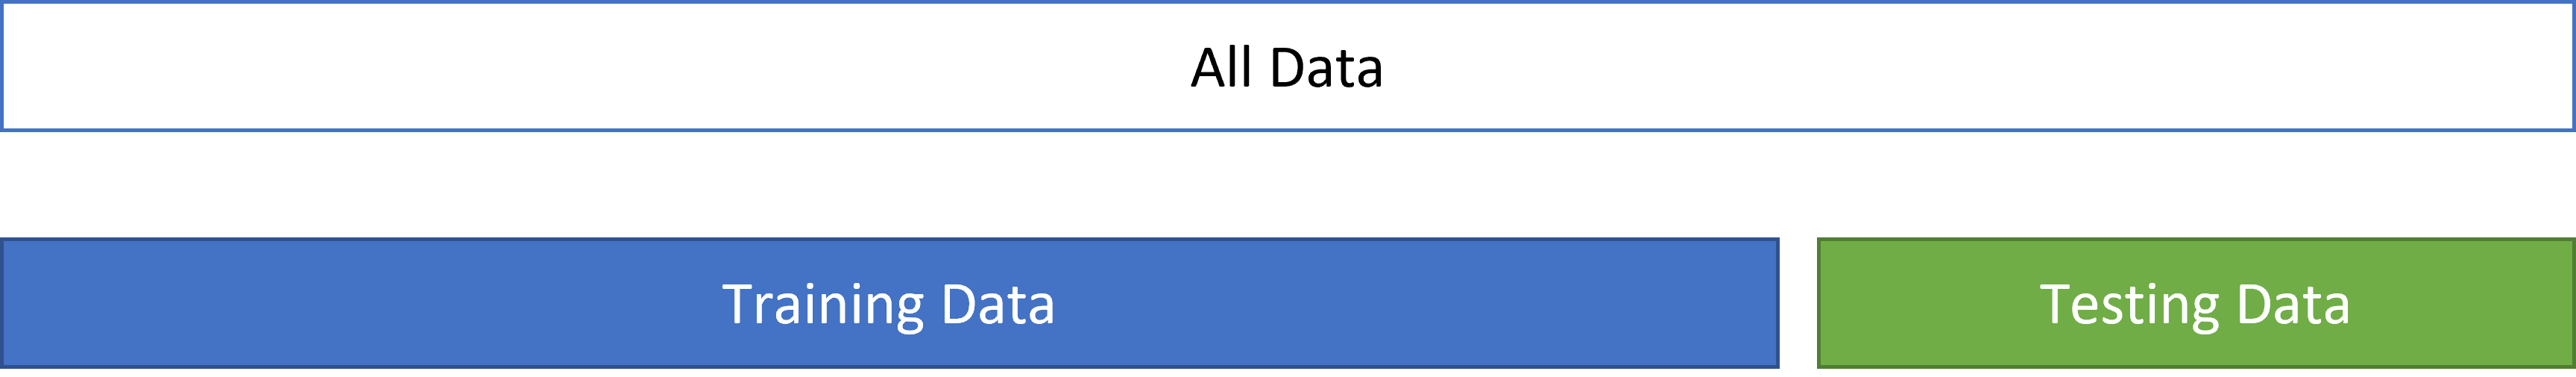
\includegraphics[width=\textwidth,height=\textheight,keepaspectratio]{figures/Train-Test split.png}
    \end{center}
\end{frame}
\begin{frame}[fragile]{Classical Machine Learning}
    \textbf{Train-Test Split}
    \href{https://scikit-learn.org/stable/modules/generated/sklearn.model_selection.train_test_split.html}{\textbf{\underline{sklearn.model\_selection.train\_test\_split}}}
    \begin{example}
        \begin{lstlisting}[language=Python]
from sklearn.model_selection import train_test_split

# Split dataset into training and testing sets
X_train, X_test, y_train, y_test = train_test_split(
X, y, test_size=0.33,
random_state=42, shuffle=True)

# Split only input samples
X_train, X_test = train_test_split(X, shuffle=False)
        \end{lstlisting}
    \end{example}
\end{frame}
\begin{frame}[fragile]{Classical Machine Learning}
    \textbf{Cross-Validation}
    However, train-test splitting would only work if the overall dataset is large enough to provide enough training samples after the split and the data is evenly distributed. To overcome this problem, a procedure called K-Fold Cross-Validation can be used wherein the data set is partitioned into K, nearly identical size sub-datasets.
    \begin{center}
        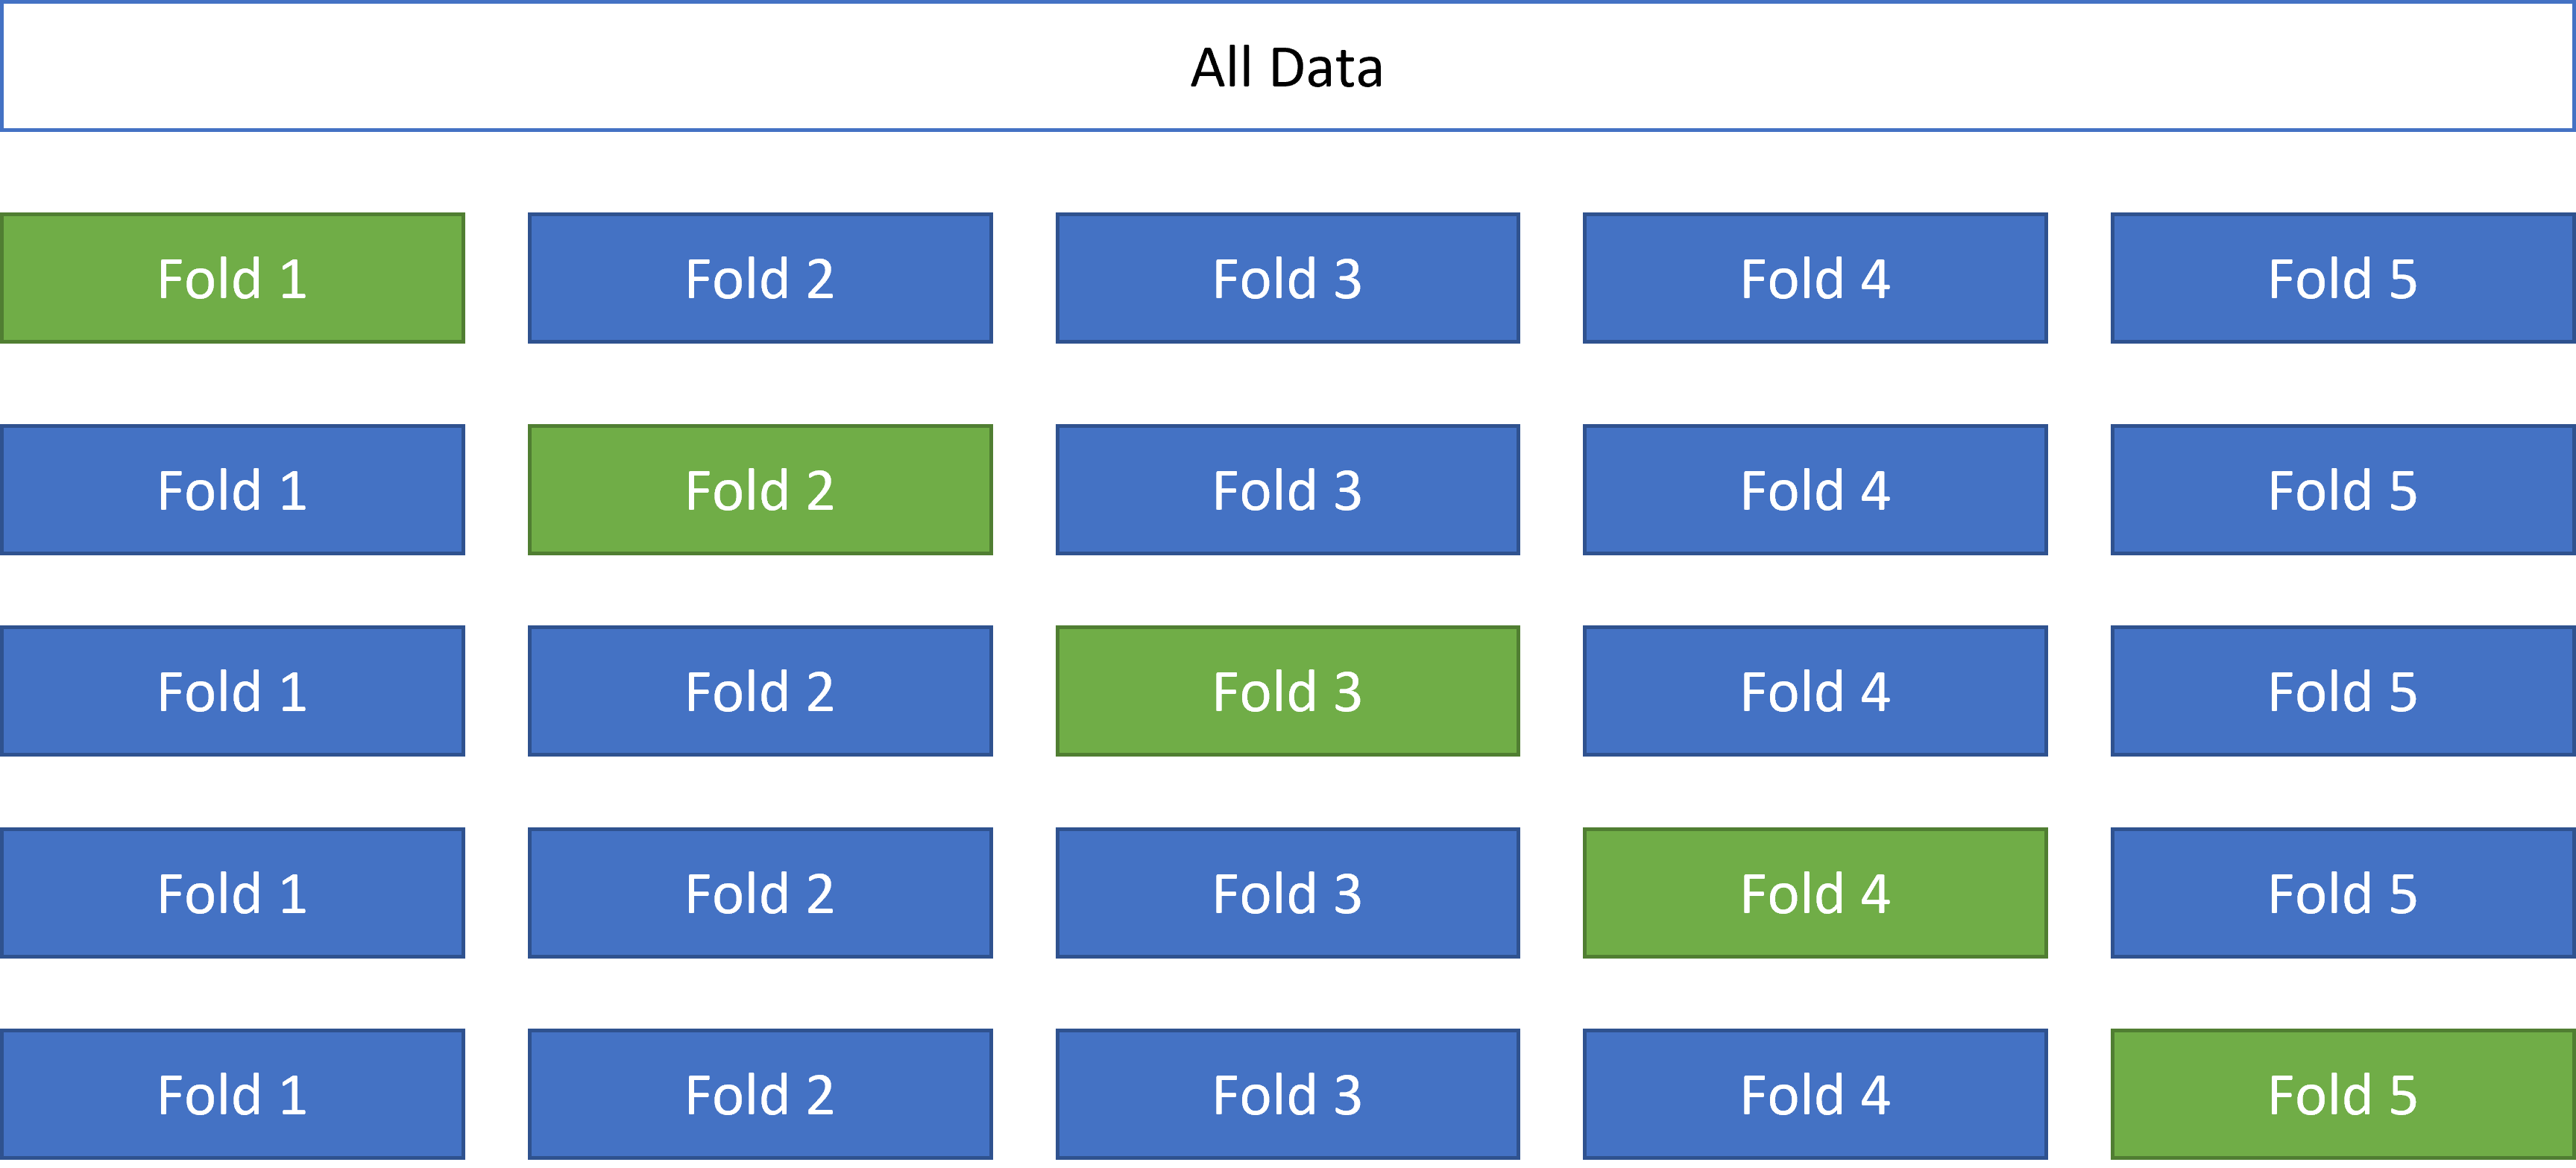
\includegraphics[width=0.8\textwidth,height=\textheight,keepaspectratio]{figures/CV.png}
    \end{center}
\end{frame}
\begin{frame}[fragile]{Classical Machine Learning}
    \textbf{Cross-Validation}
    \href{https://scikit-learn.org/stable/modules/generated/sklearn.model_selection.cross_val_score.html}{\textbf{\underline{sklearn.model\_selection.cross\_val\_score}}}
    \begin{example}
        \begin{lstlisting}[language=Python]
from sklearn.model_selection import cross_val_score

# Load dataset
X, y = load_dataset()

# Build model
model = build_model()

# CV scores
cv_scores = cross_val_score(model, X, y, cv=5)
        \end{lstlisting}
    \end{example}
\end{frame}
\subsection{Modern Machine Learning}
\begin{frame}[fragile]{Intro to Machine Learning}
    \begin{center}
        \Huge Contemporary (Deep) Machine Learning
    \end{center}
\end{frame}
\begin{frame}[fragile]{What is Deep Learning?}
    As discussed in the previous section, Classical Machine Learning models rely on 
    \begin{itemize}
        \item Prior Domain Knowledge
        \item Specific Data Distribution
        \item Hand Engineered Features
    \end{itemize}
    To produce an overdetermined model that works with a minimal amount of data. However, the primary limit of Classical Machine Learning is the model's complexities and scalabilities.
\end{frame}
\begin{frame}[fragile]{What is Deep Learning?}
    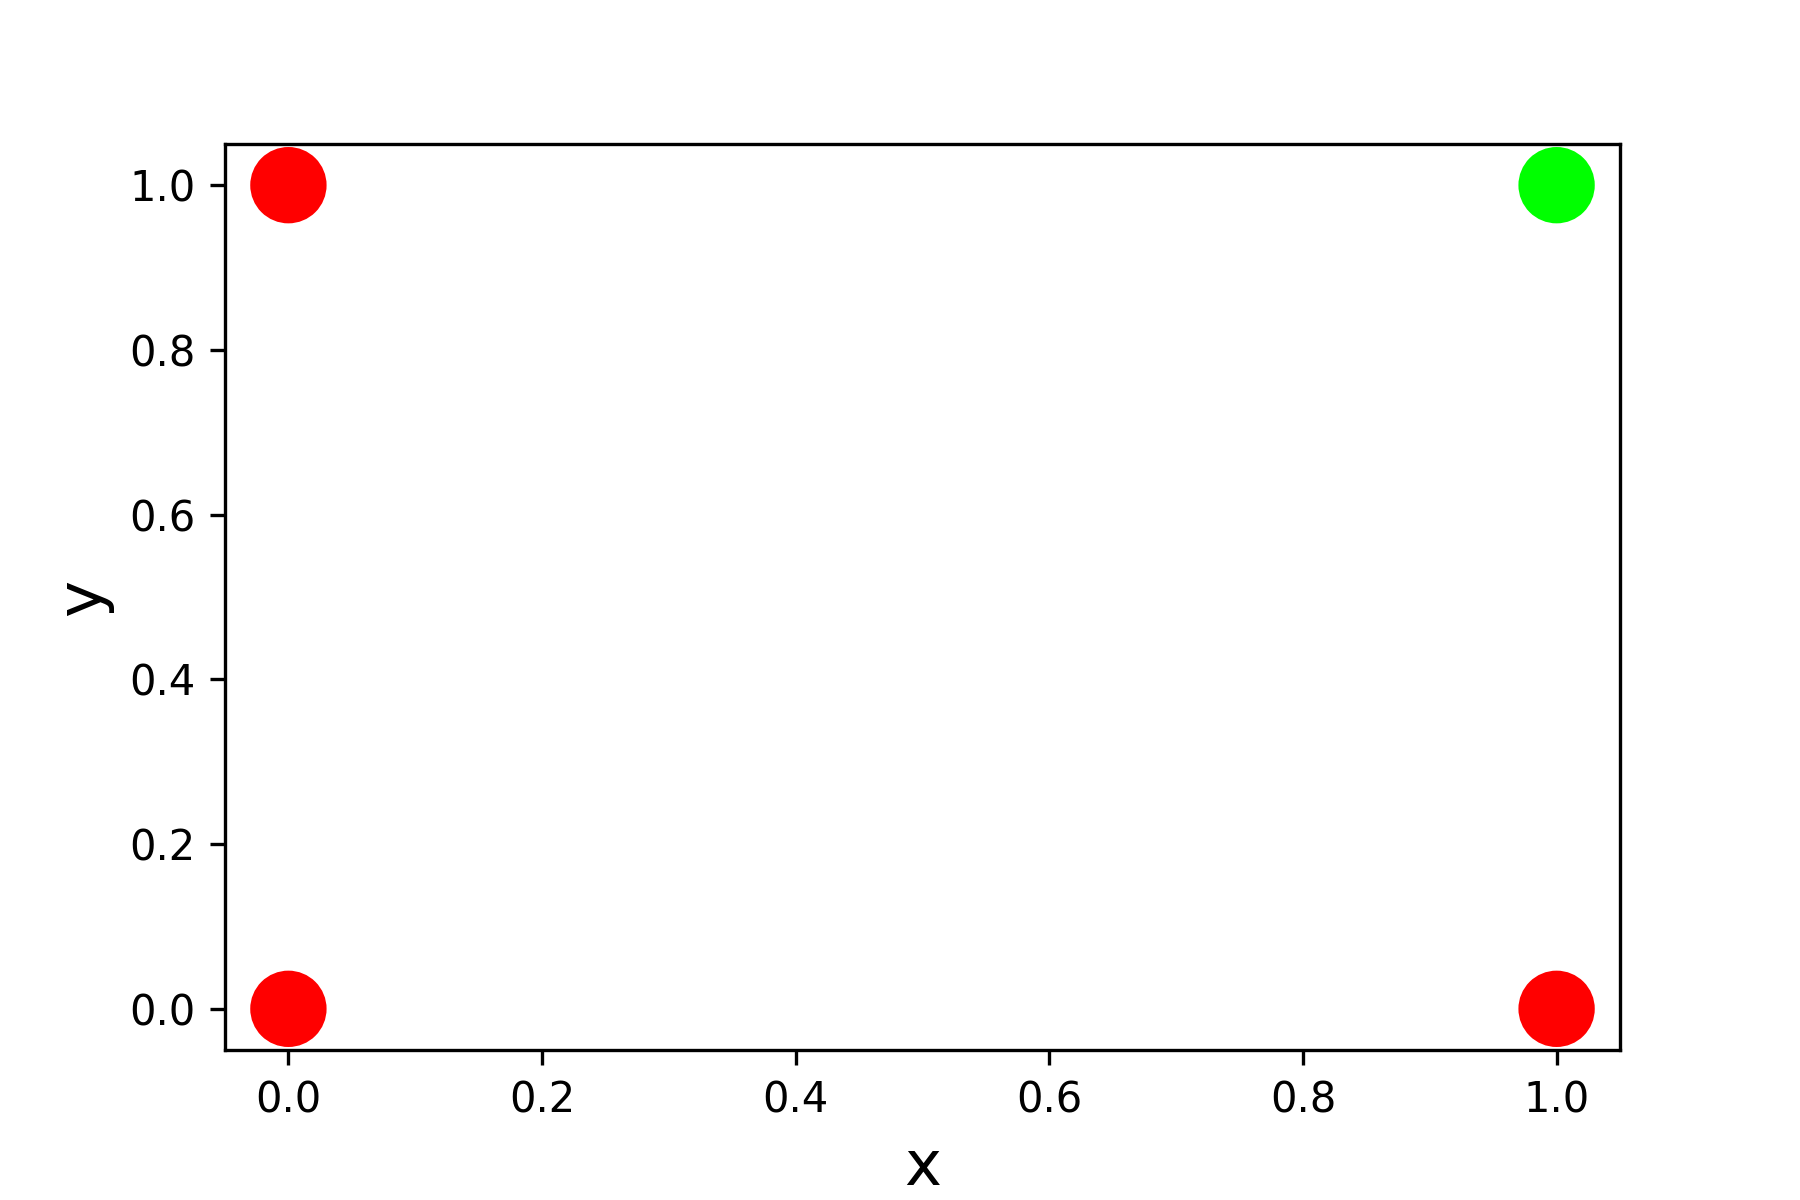
\includegraphics[width=0.48\textwidth,height=\textheight,keepaspectratio]{figures/And Example.png}
    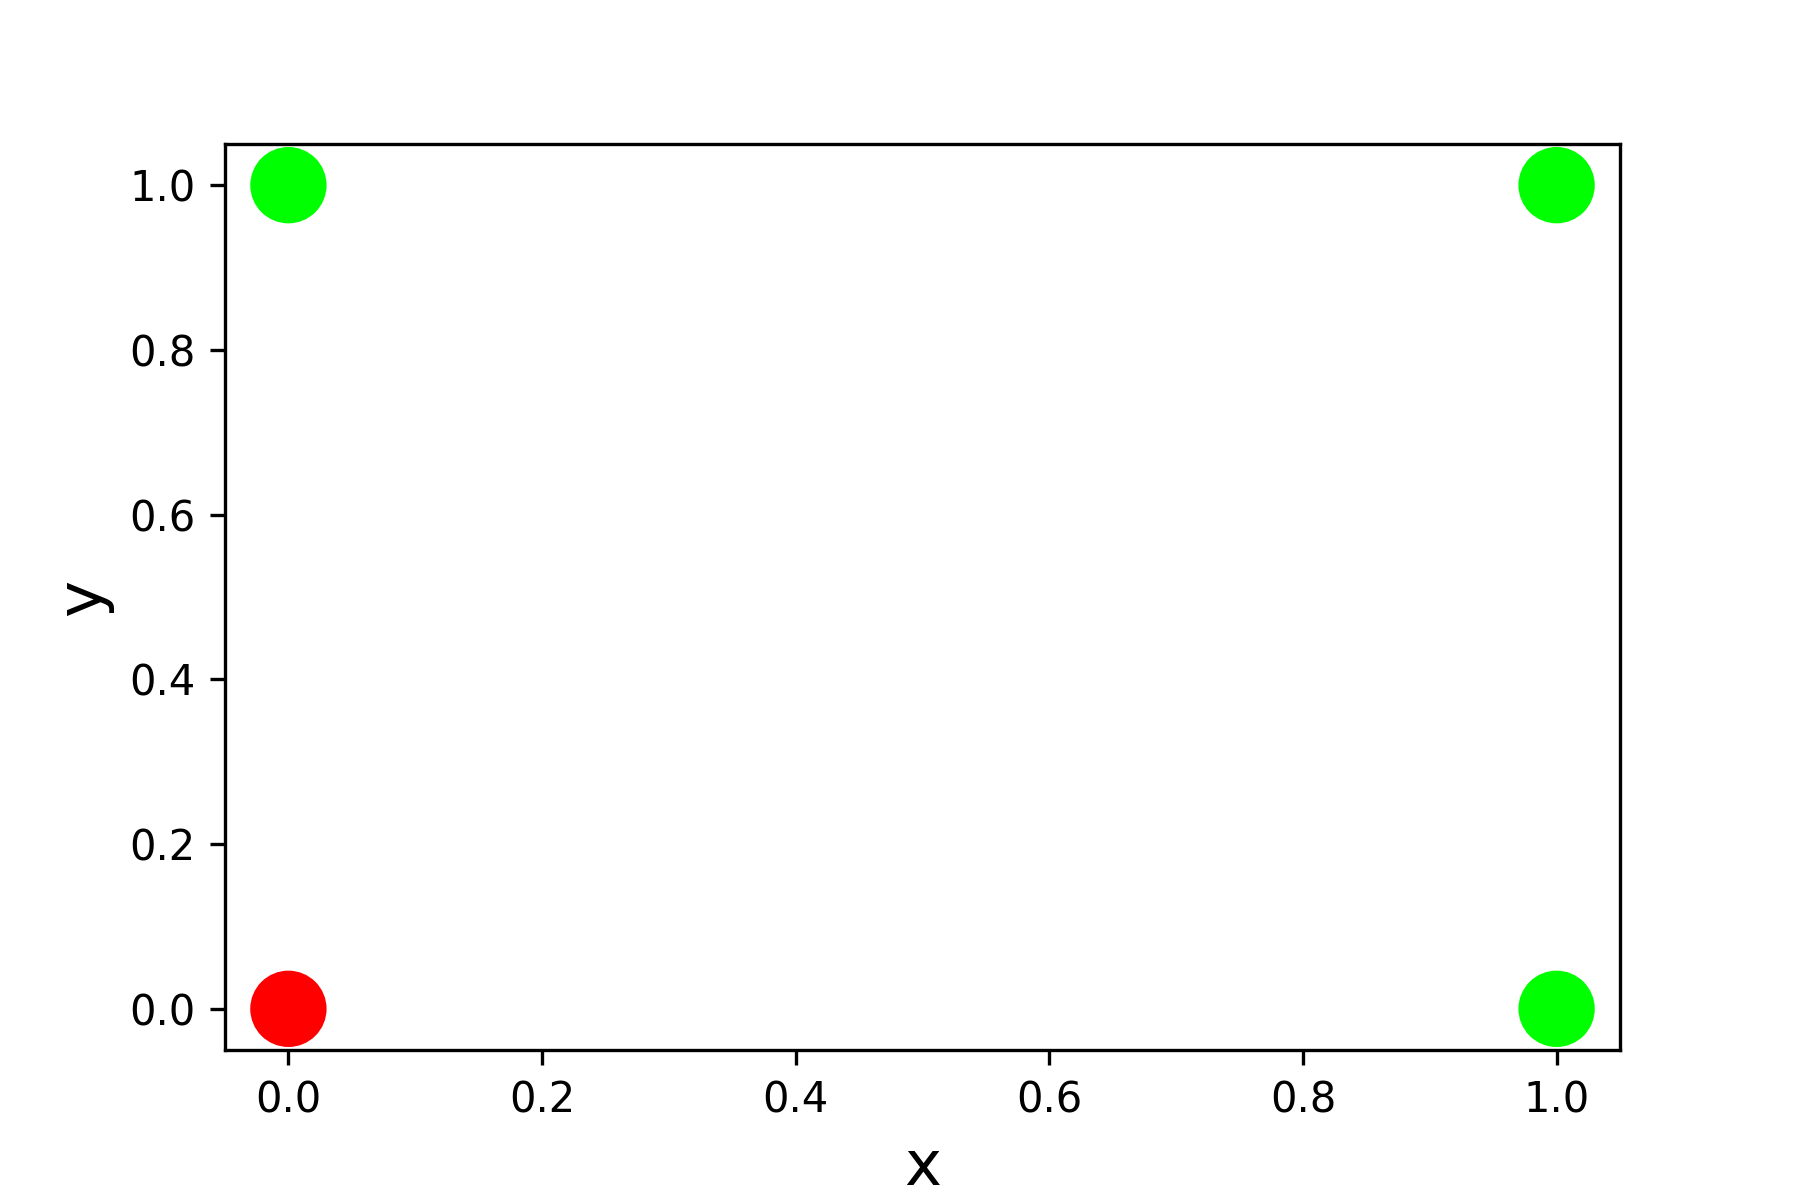
\includegraphics[width=0.48\textwidth,height=\textheight,keepaspectratio]{figures/Or Example.png}
\end{frame}
\begin{frame}[fragile]{What is Deep Learning?}
    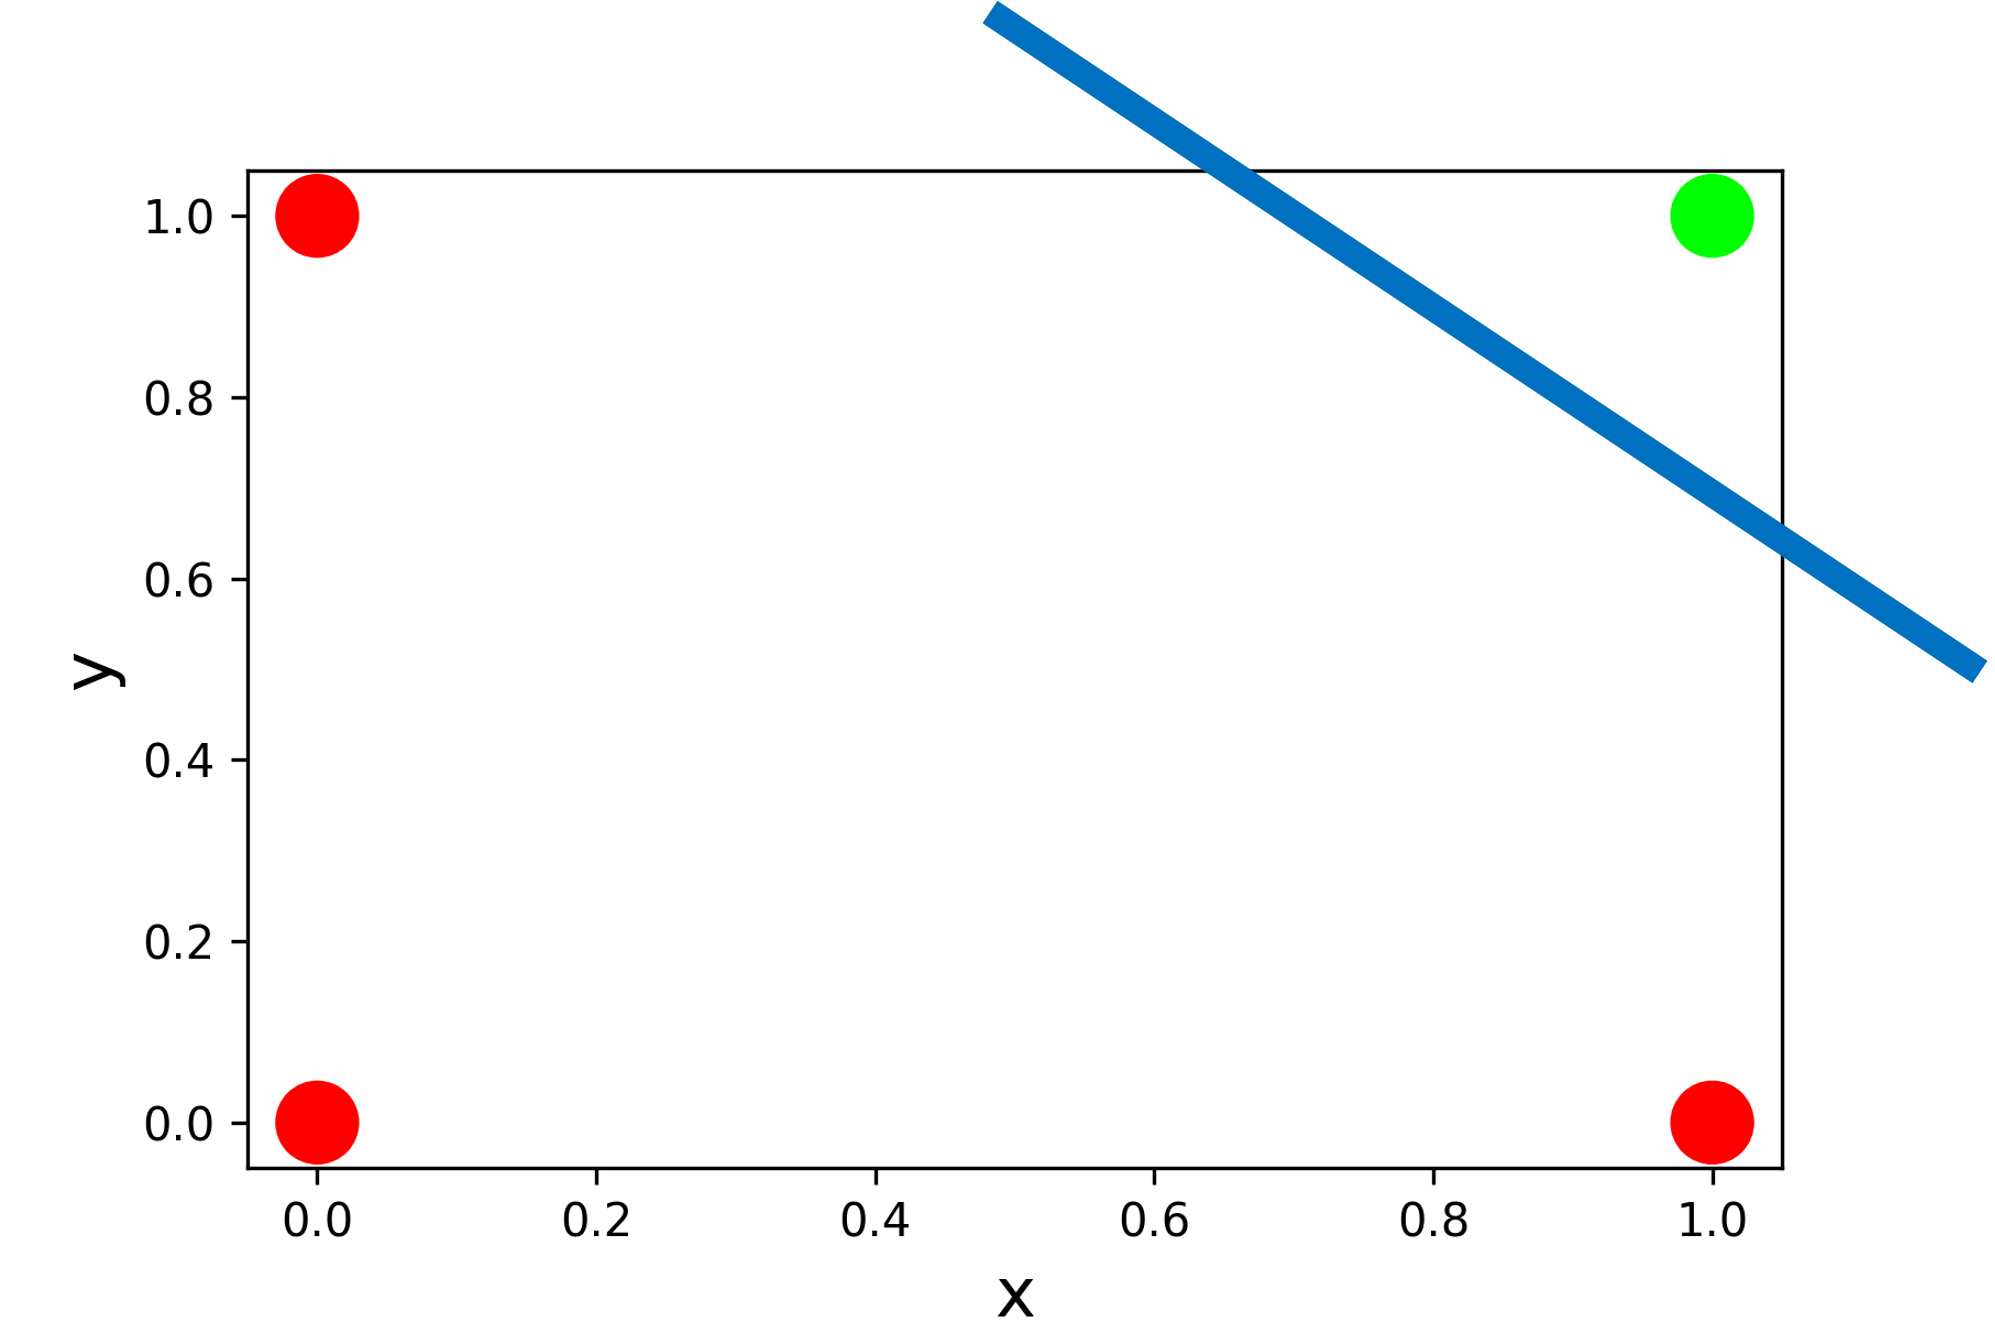
\includegraphics[width=0.48\textwidth,height=\textheight,keepaspectratio]{figures/And Example 2.png}
    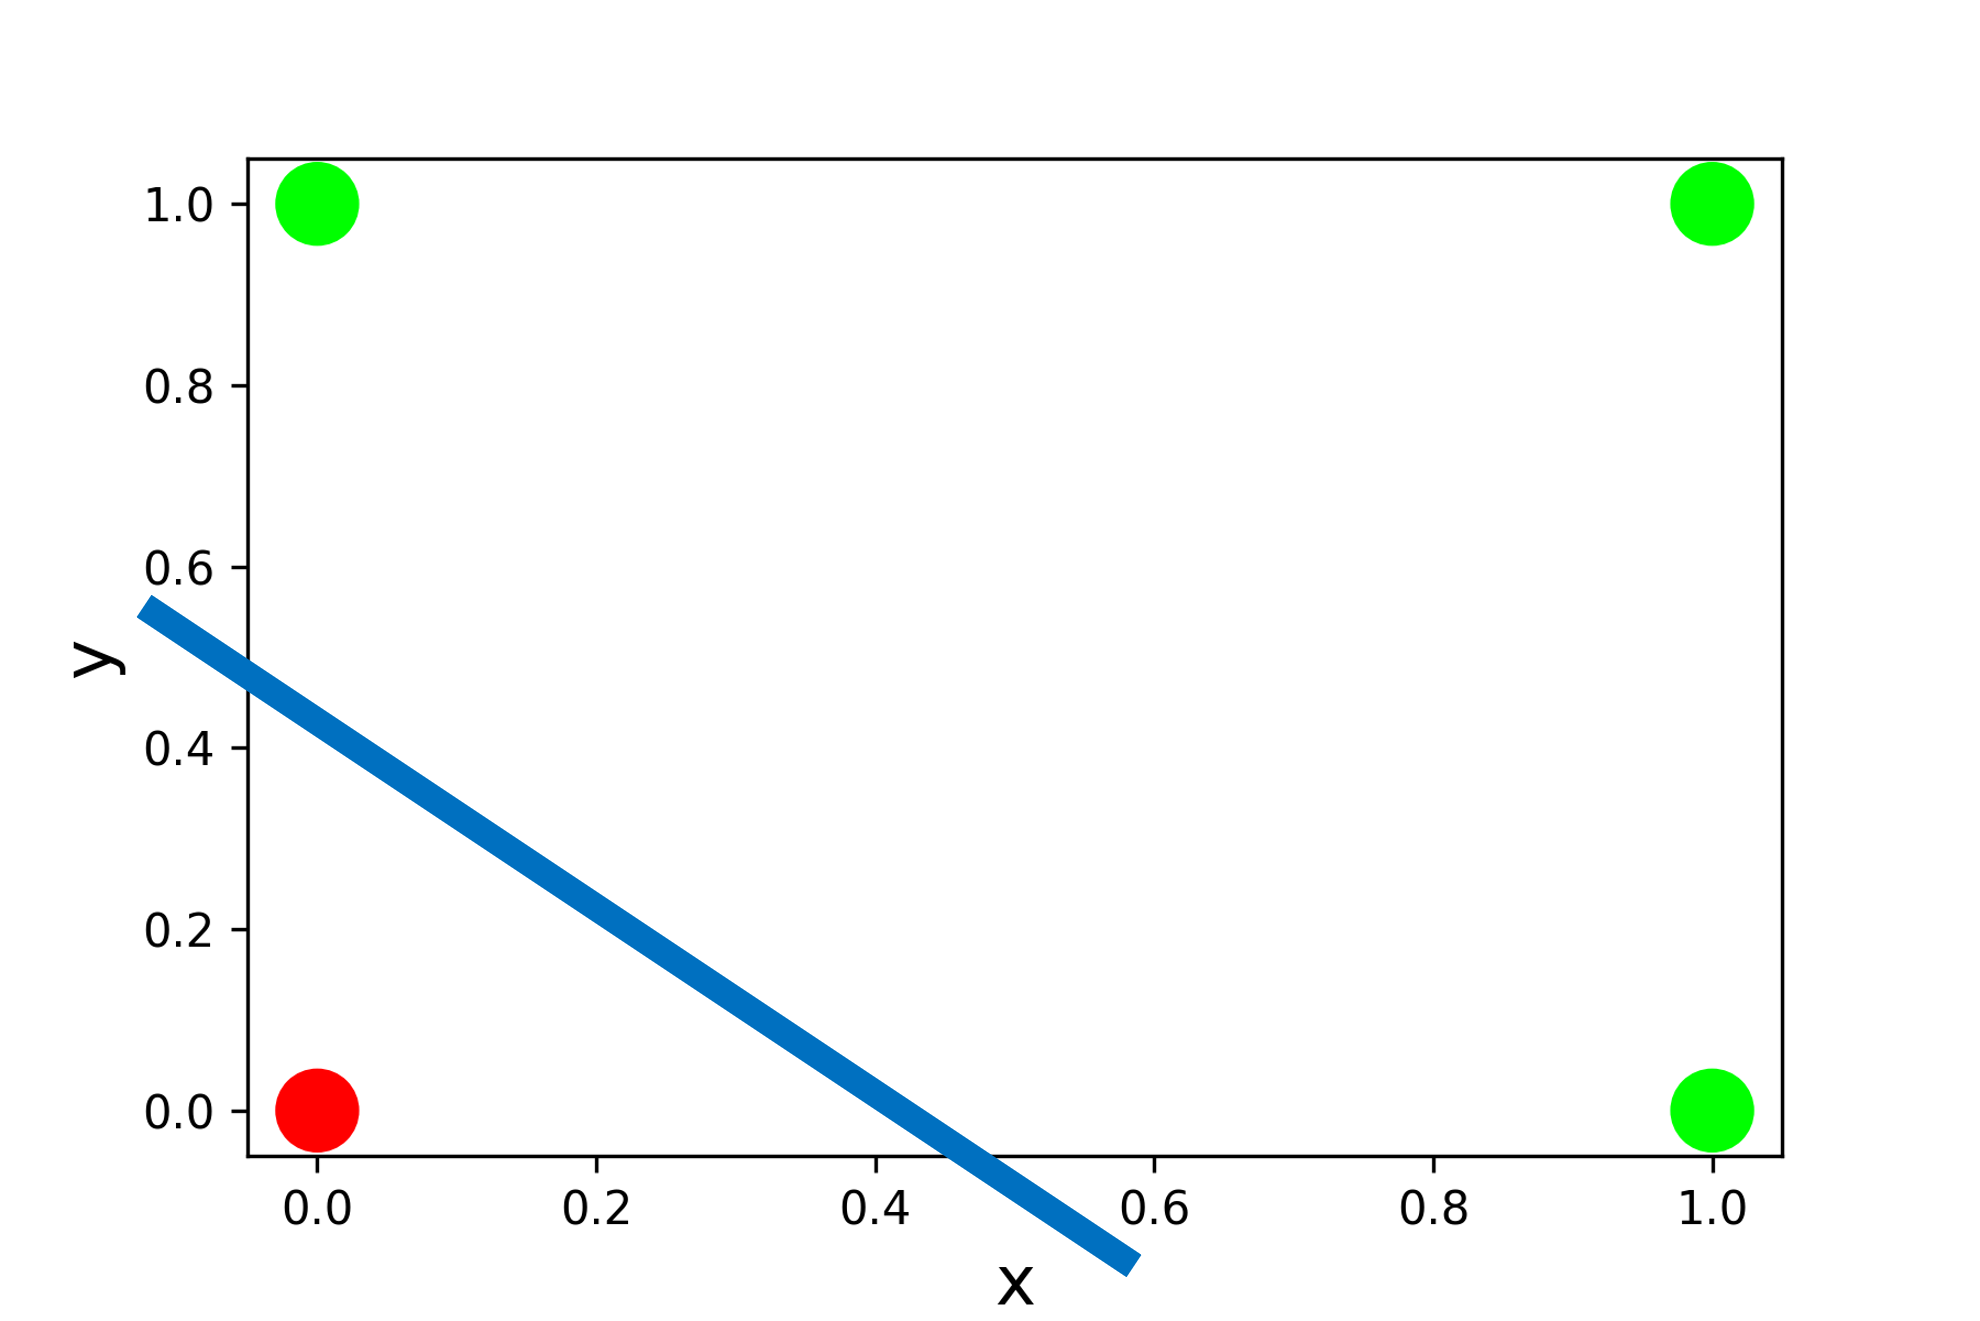
\includegraphics[width=0.48\textwidth,height=\textheight,keepaspectratio]{figures/Or Example 2.png}
\end{frame}
\begin{frame}[fragile]{What is Deep Learning?}
    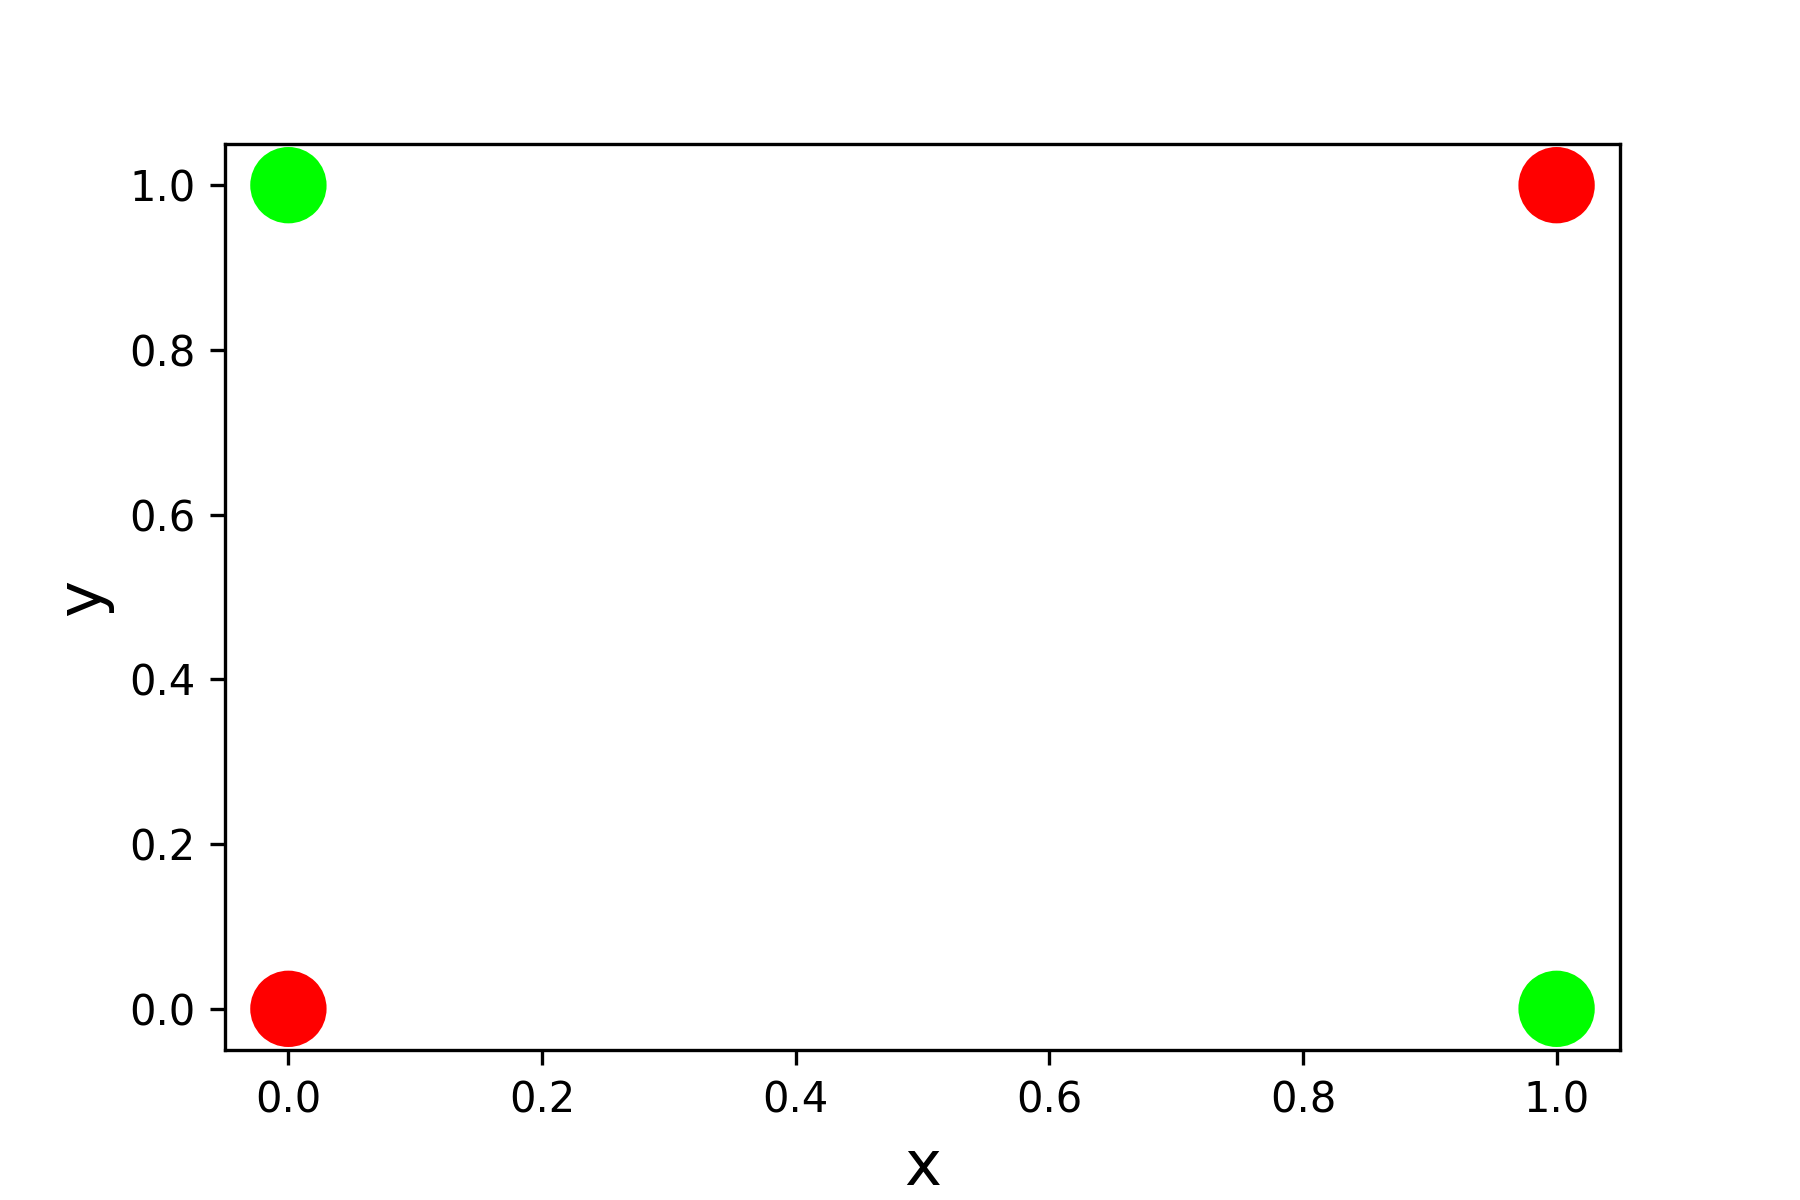
\includegraphics[width=\textwidth,height=\textheight,keepaspectratio]{figures/Xor Example.png}
\end{frame}
\begin{frame}[fragile]{What is Deep Learning?}
    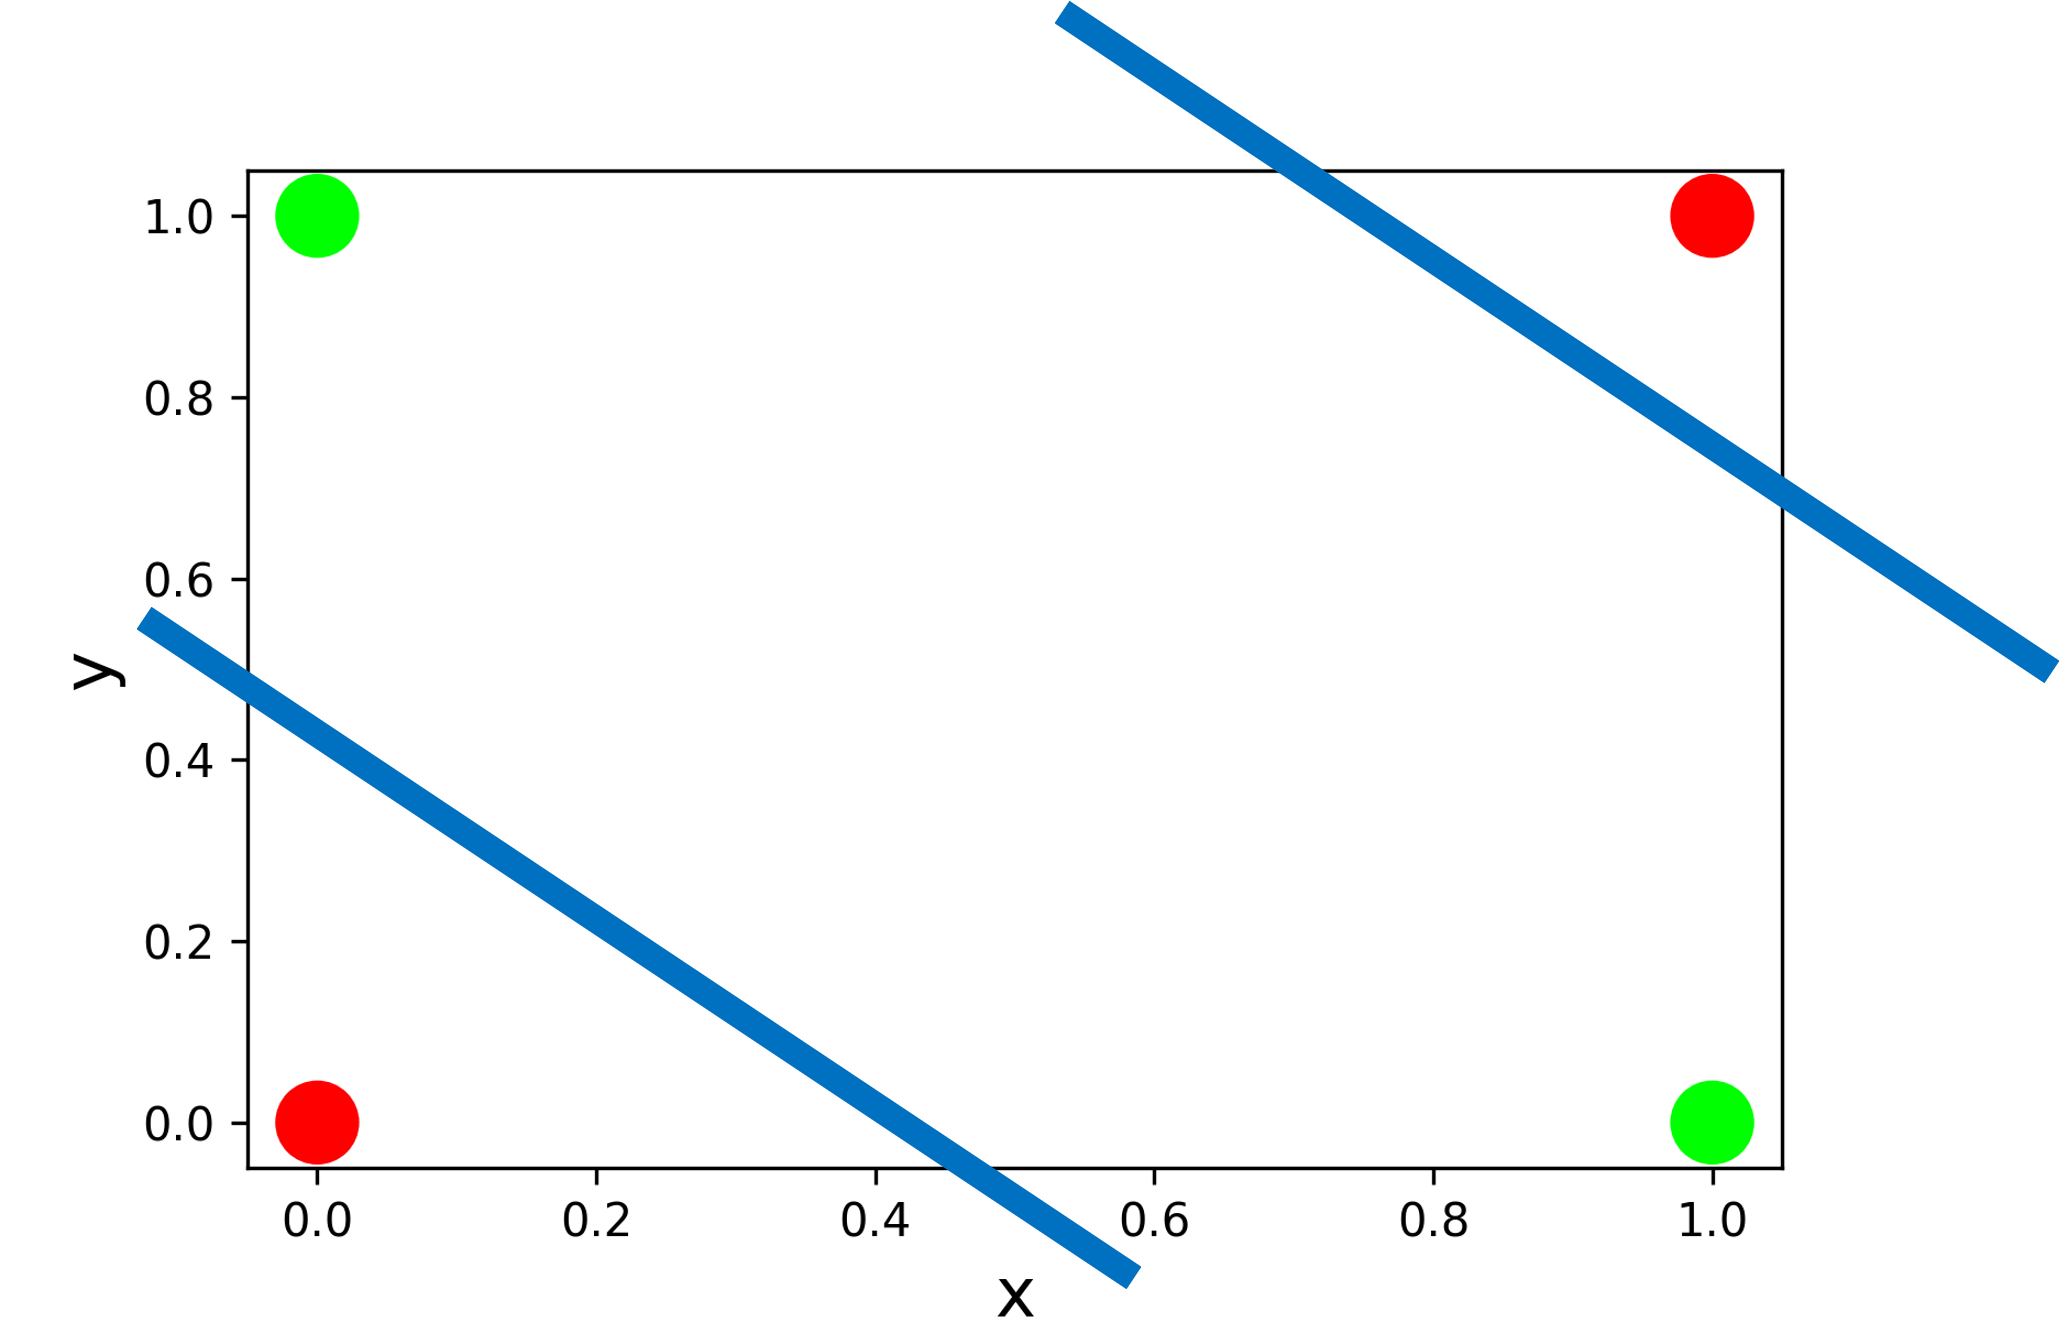
\includegraphics[width=\textwidth,height=\textheight,keepaspectratio]{figures/Xor Example 2.png}
\end{frame}
\begin{frame}[fragile]{What is Deep Learning?}
    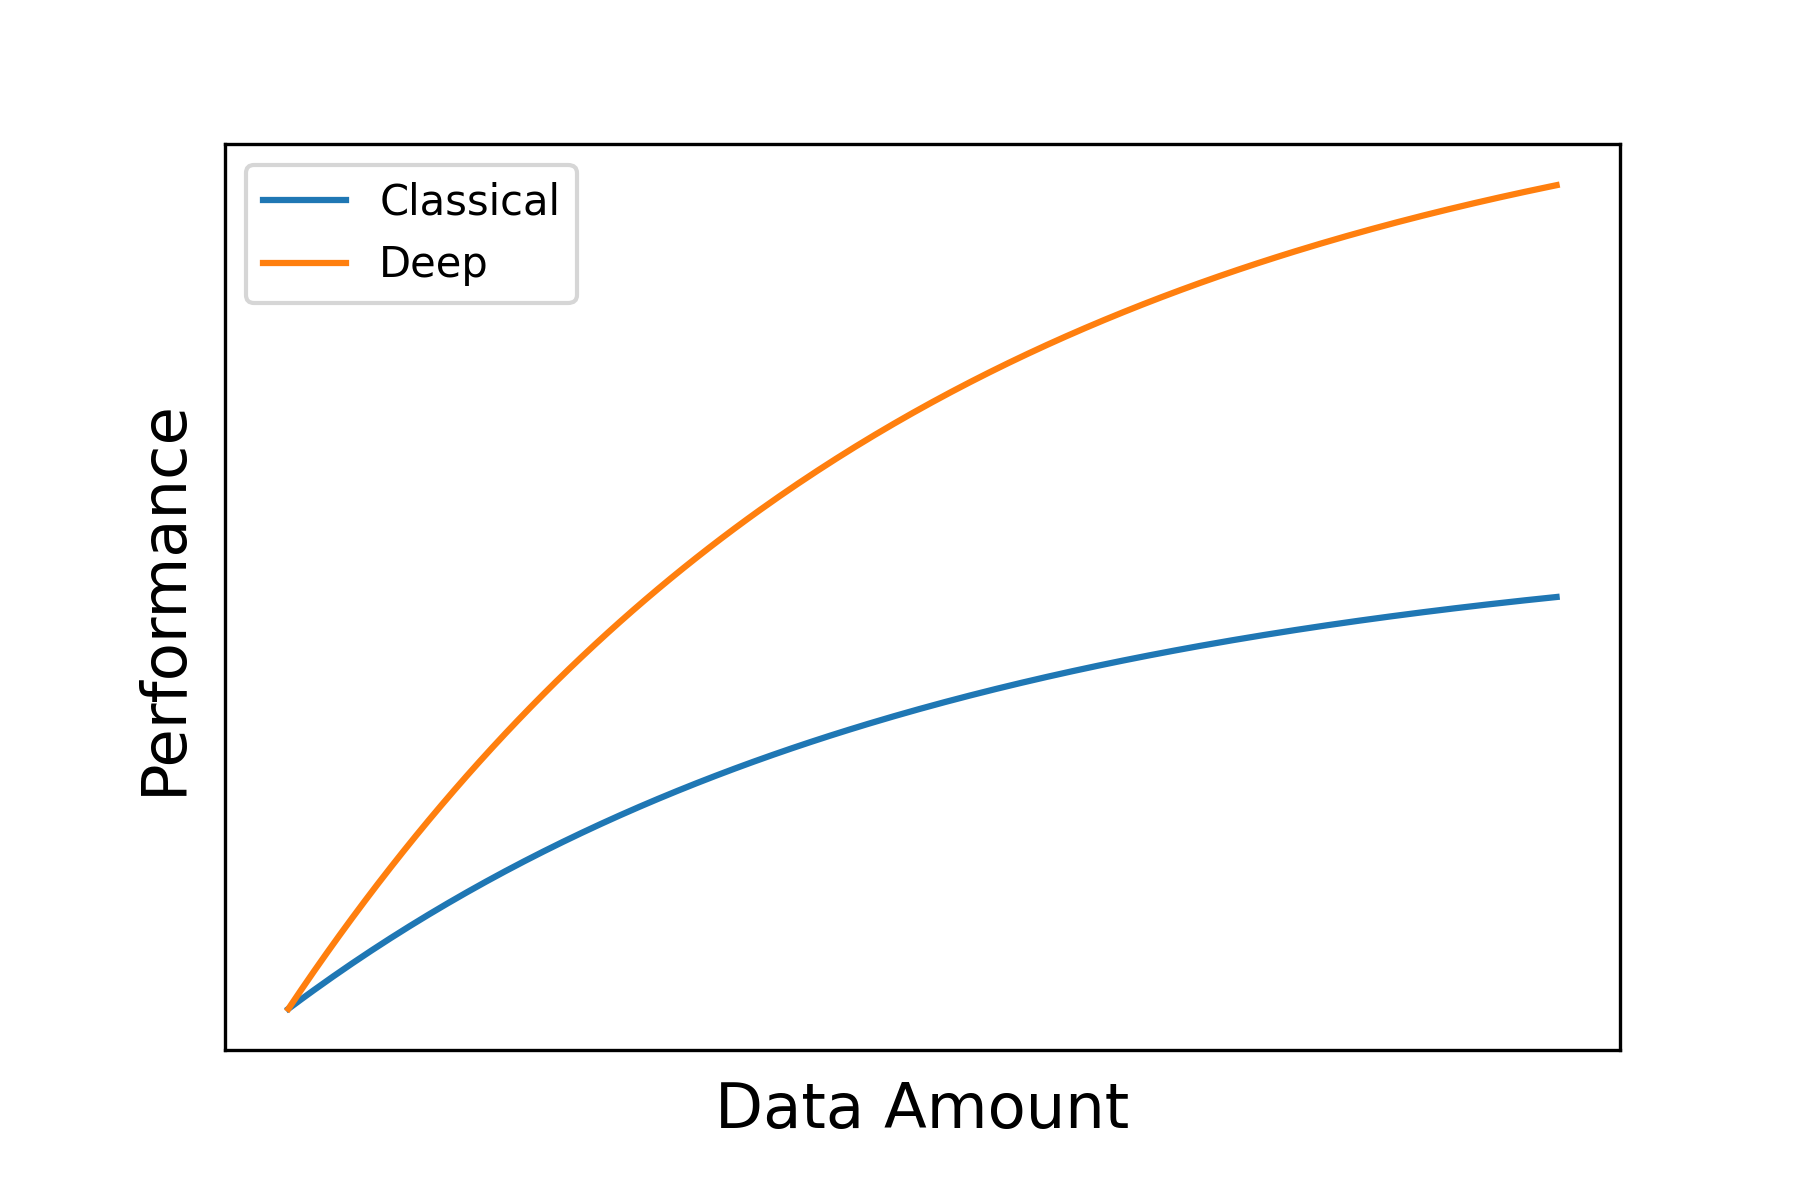
\includegraphics[width=\textwidth,height=\textheight,keepaspectratio]{figures/Deep vs Classical.png}
\end{frame}
\begin{frame}[fragile]{What is Deep Learning?}
    How to solve complexities and scalabilities problems?
    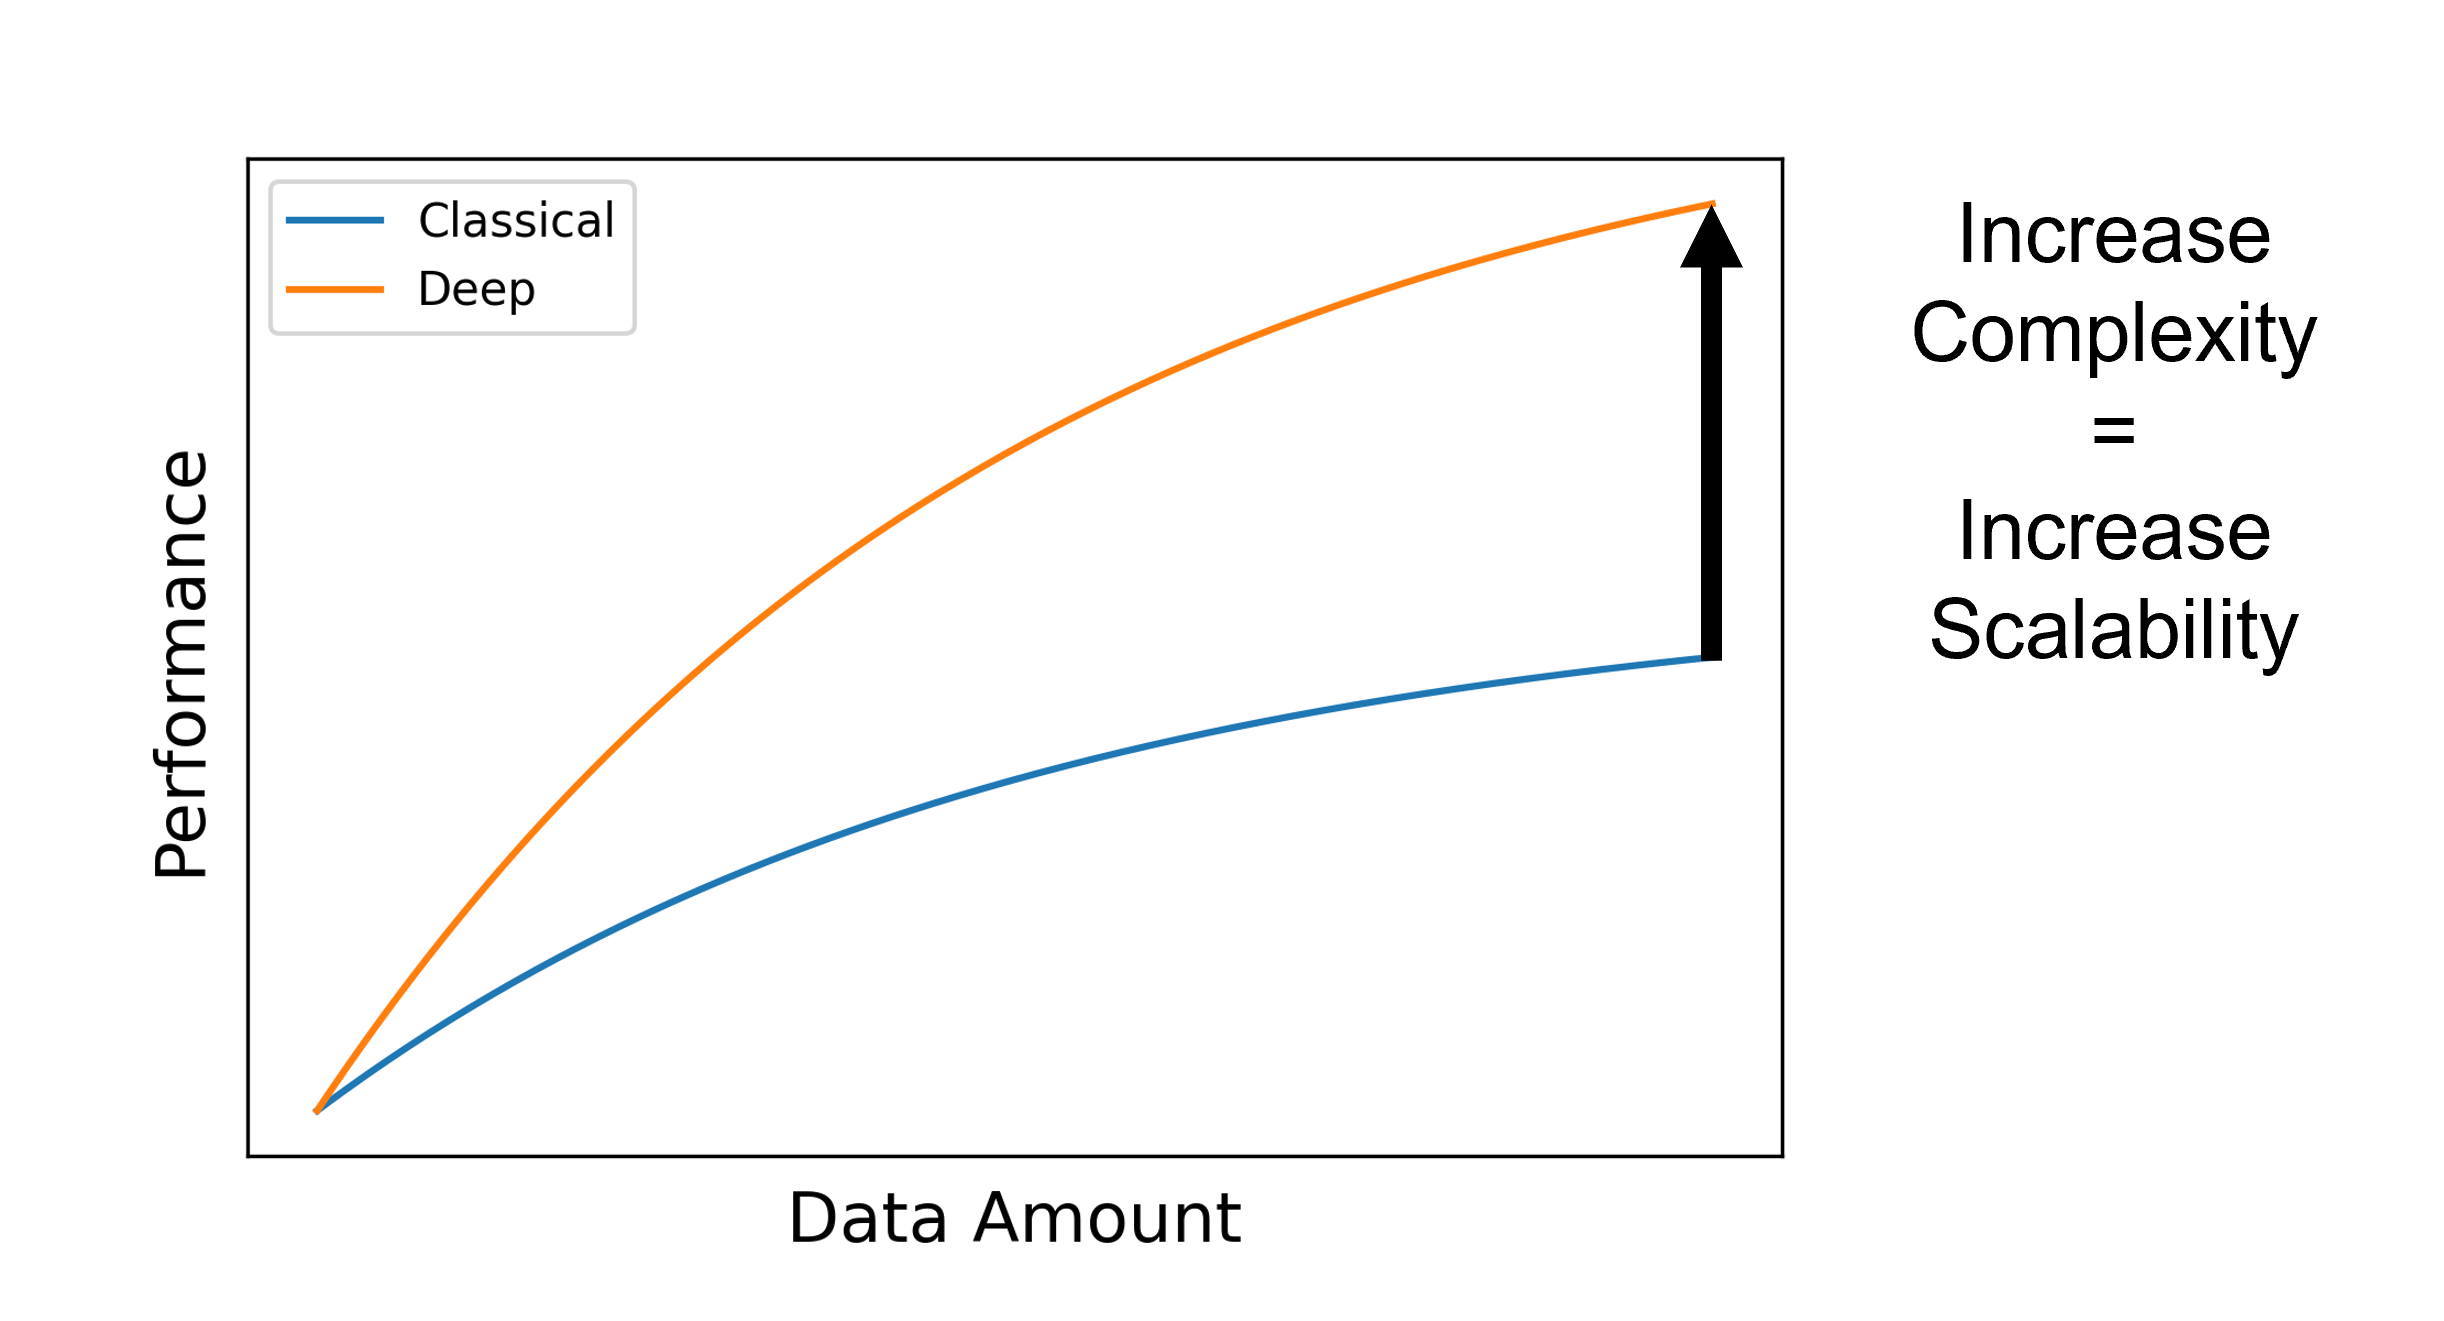
\includegraphics[width=\textwidth,height=\textheight,keepaspectratio]{figures/Deep vs Classical 2.png}
\end{frame}

\begin{frame}[fragile]{What is Deep Learning?}
    \textbf{Deep Learning} is a class of machine learning algorithms inspired by the brain's structure and function. It uses deep architecture to achieve high complexities and relies on large amounts of data to train an underdetermined model. The "stacking" of hidden layers allows Deep learning models to increase their model complexities exponentially, enabling the model to emulate real-life functions to an unprecedented degree. In contrast to Classical Machine Learning, Deep Learning doesn't rely on the following:
    \begin{itemize}
        \item Specific Data Distribution
        \item Hand Engineered Features
    \end{itemize}
    The "stacking" of hidden layers allows Deep learning models to increase their model complexities exponentially, enabling the model to emulate real-life functions to an unprecedented degree.
\end{frame}
\begin{frame}[fragile]{What is Deep Learning?}
    \begin{block}{For Me}
        Deep Learning model is a bunch of nested composite functions.\\
        \begin{equation*}
            \hat{y} = f_{n}(f_{n-1}(f_{n-2}(\cdots f_{1}(x)\cdots)))
        \end{equation*}
        with $n$ being the number of layers.
    \end{block}
\end{frame}
\begin{frame}[fragile]{Weights Update}
    \textbf{How do we update the weights(parameters) an underdetermined model?}\\
    In Linear models, we use the least squares method, which uses derivatives to find the optimal weights that minimize the error between the model output and the target data.
    % \begin{equation}
    %     \hat{W}^{T} = (X^{T}X)^{-1}X^{T}Y
    % \end{equation}
    However, this method is moot in Deep Learning since most models are underdetermined.
\end{frame}
\begin{frame}[fragile]{Iterative Optimization Algorithm}
    % \big{Iterative Optimization Algorithm}
    \textbf{Iterative Optimization Algorithm} is a method to find the minimum of a function by iteratively updating the weights from a random starting point in a predetermined direction. The process is repeated until the weights converge. \\
    In Deep Learning, the process consists of 2 main basic methods:
    \begin{itemize}
        \item Gradient Descent
        \item Backpropagation
    \end{itemize}
\end{frame}
\begin{frame}[fragile]{Gradient Descent}
    \textbf{Gradient Descent}, or \textbf{Steepest Descent}, is a first-order iterative optimization algorithm that updates the weights by going in the opposite direction of the gradients, i.e. negative gradient. The process is repeated iteratively until the local/global minimum is found.
    % \begin{align*}
    %     W_{i+1} = W_{i} - \alpha \Delta W_{L} \\
    %     \Delta {W}_{L} = \frac{\partial L}{\partial W}
    % \end{align*}
    % \begin{block}{learning rate}
    %     The learning rate $\alpha$ is a hyperparameter that controls the step size.
    % \end{block}
\end{frame}
\begin{frame}[fragile]{Gradient Descent}
    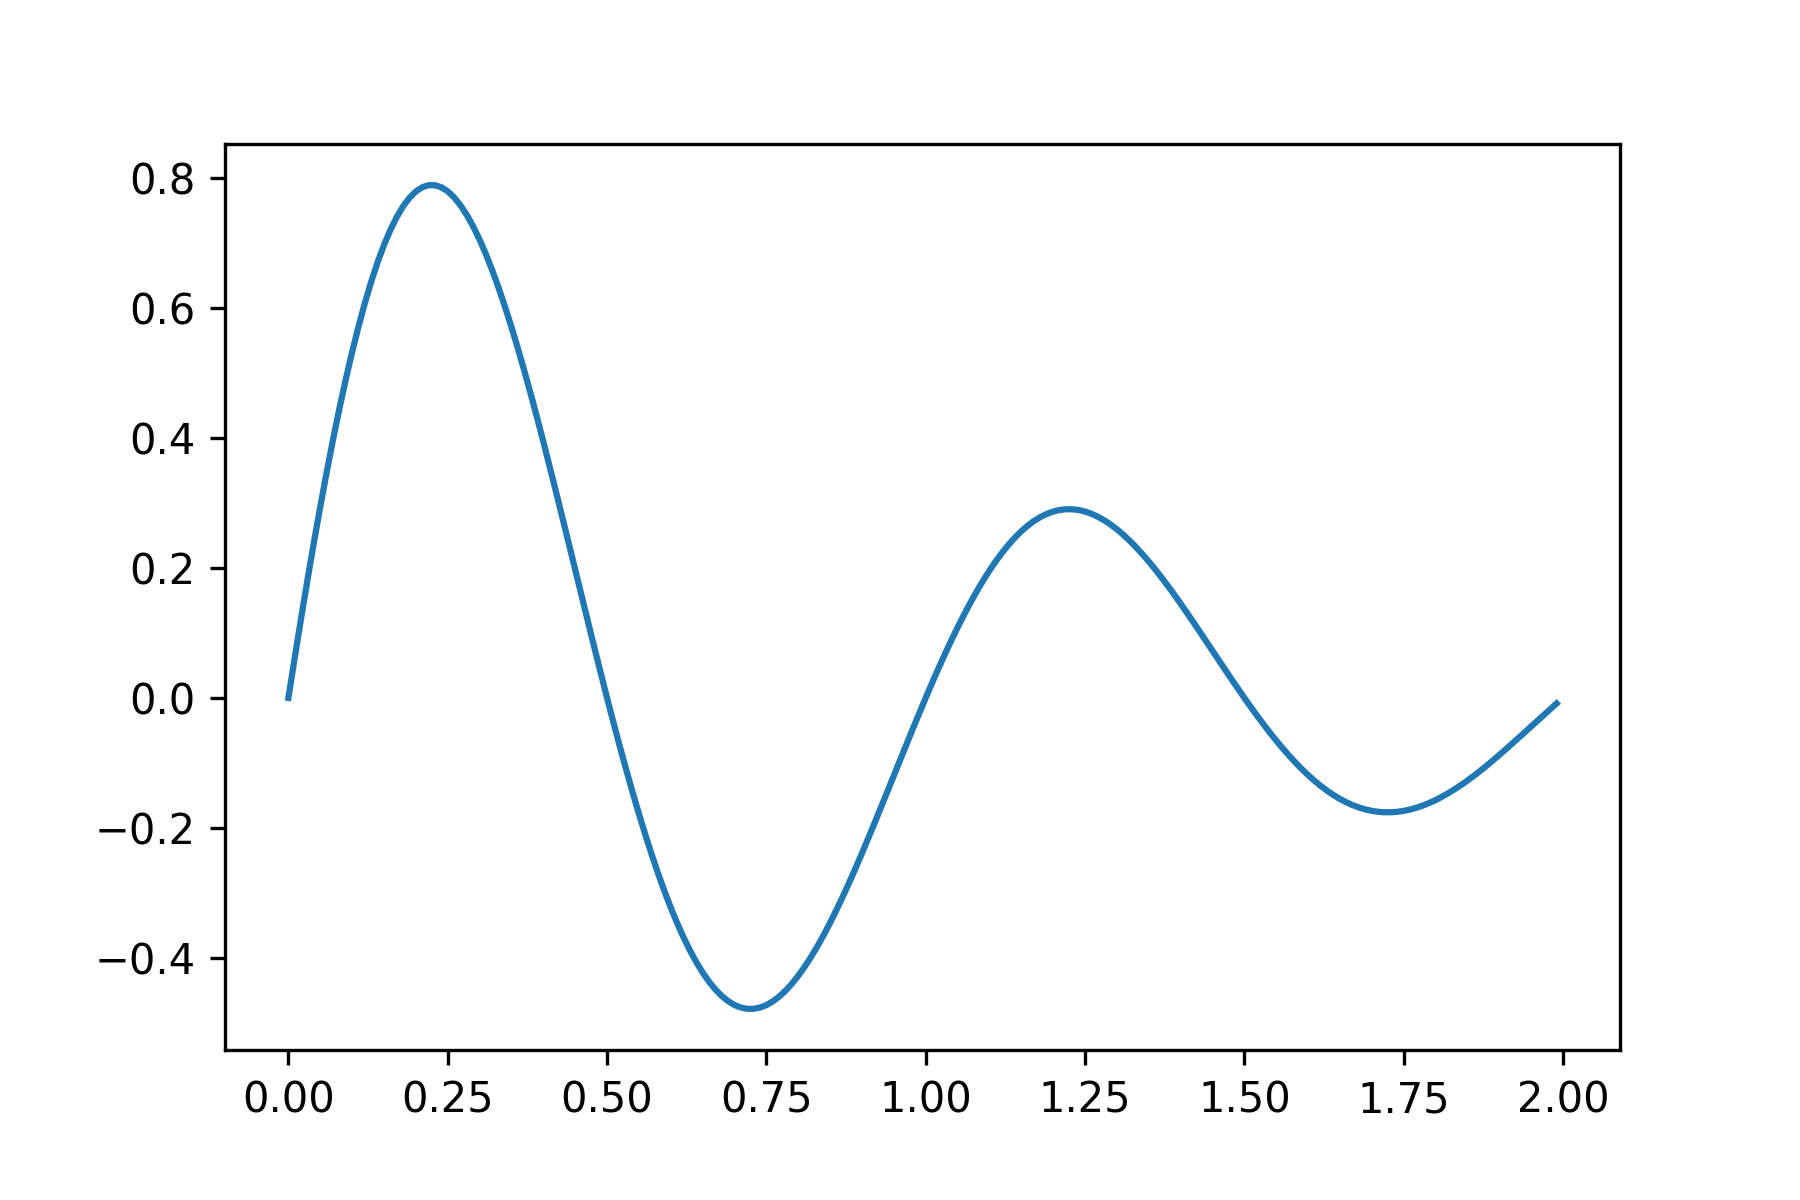
\includegraphics[width=\textwidth,height=\textheight,keepaspectratio]{figures/MinimaExample.png}
\end{frame}

\begin{frame}[fragile]{Learning Curve}
    \textbf{Learning Curve} in Machine Learning is a proxy measurement of how the learning or proficiency is progressing given experiences. Typically a learning curve is a plot between performance or loss value (Y-axis) against progression (X-axis), e.g. training samples, iterations, or epochs.
    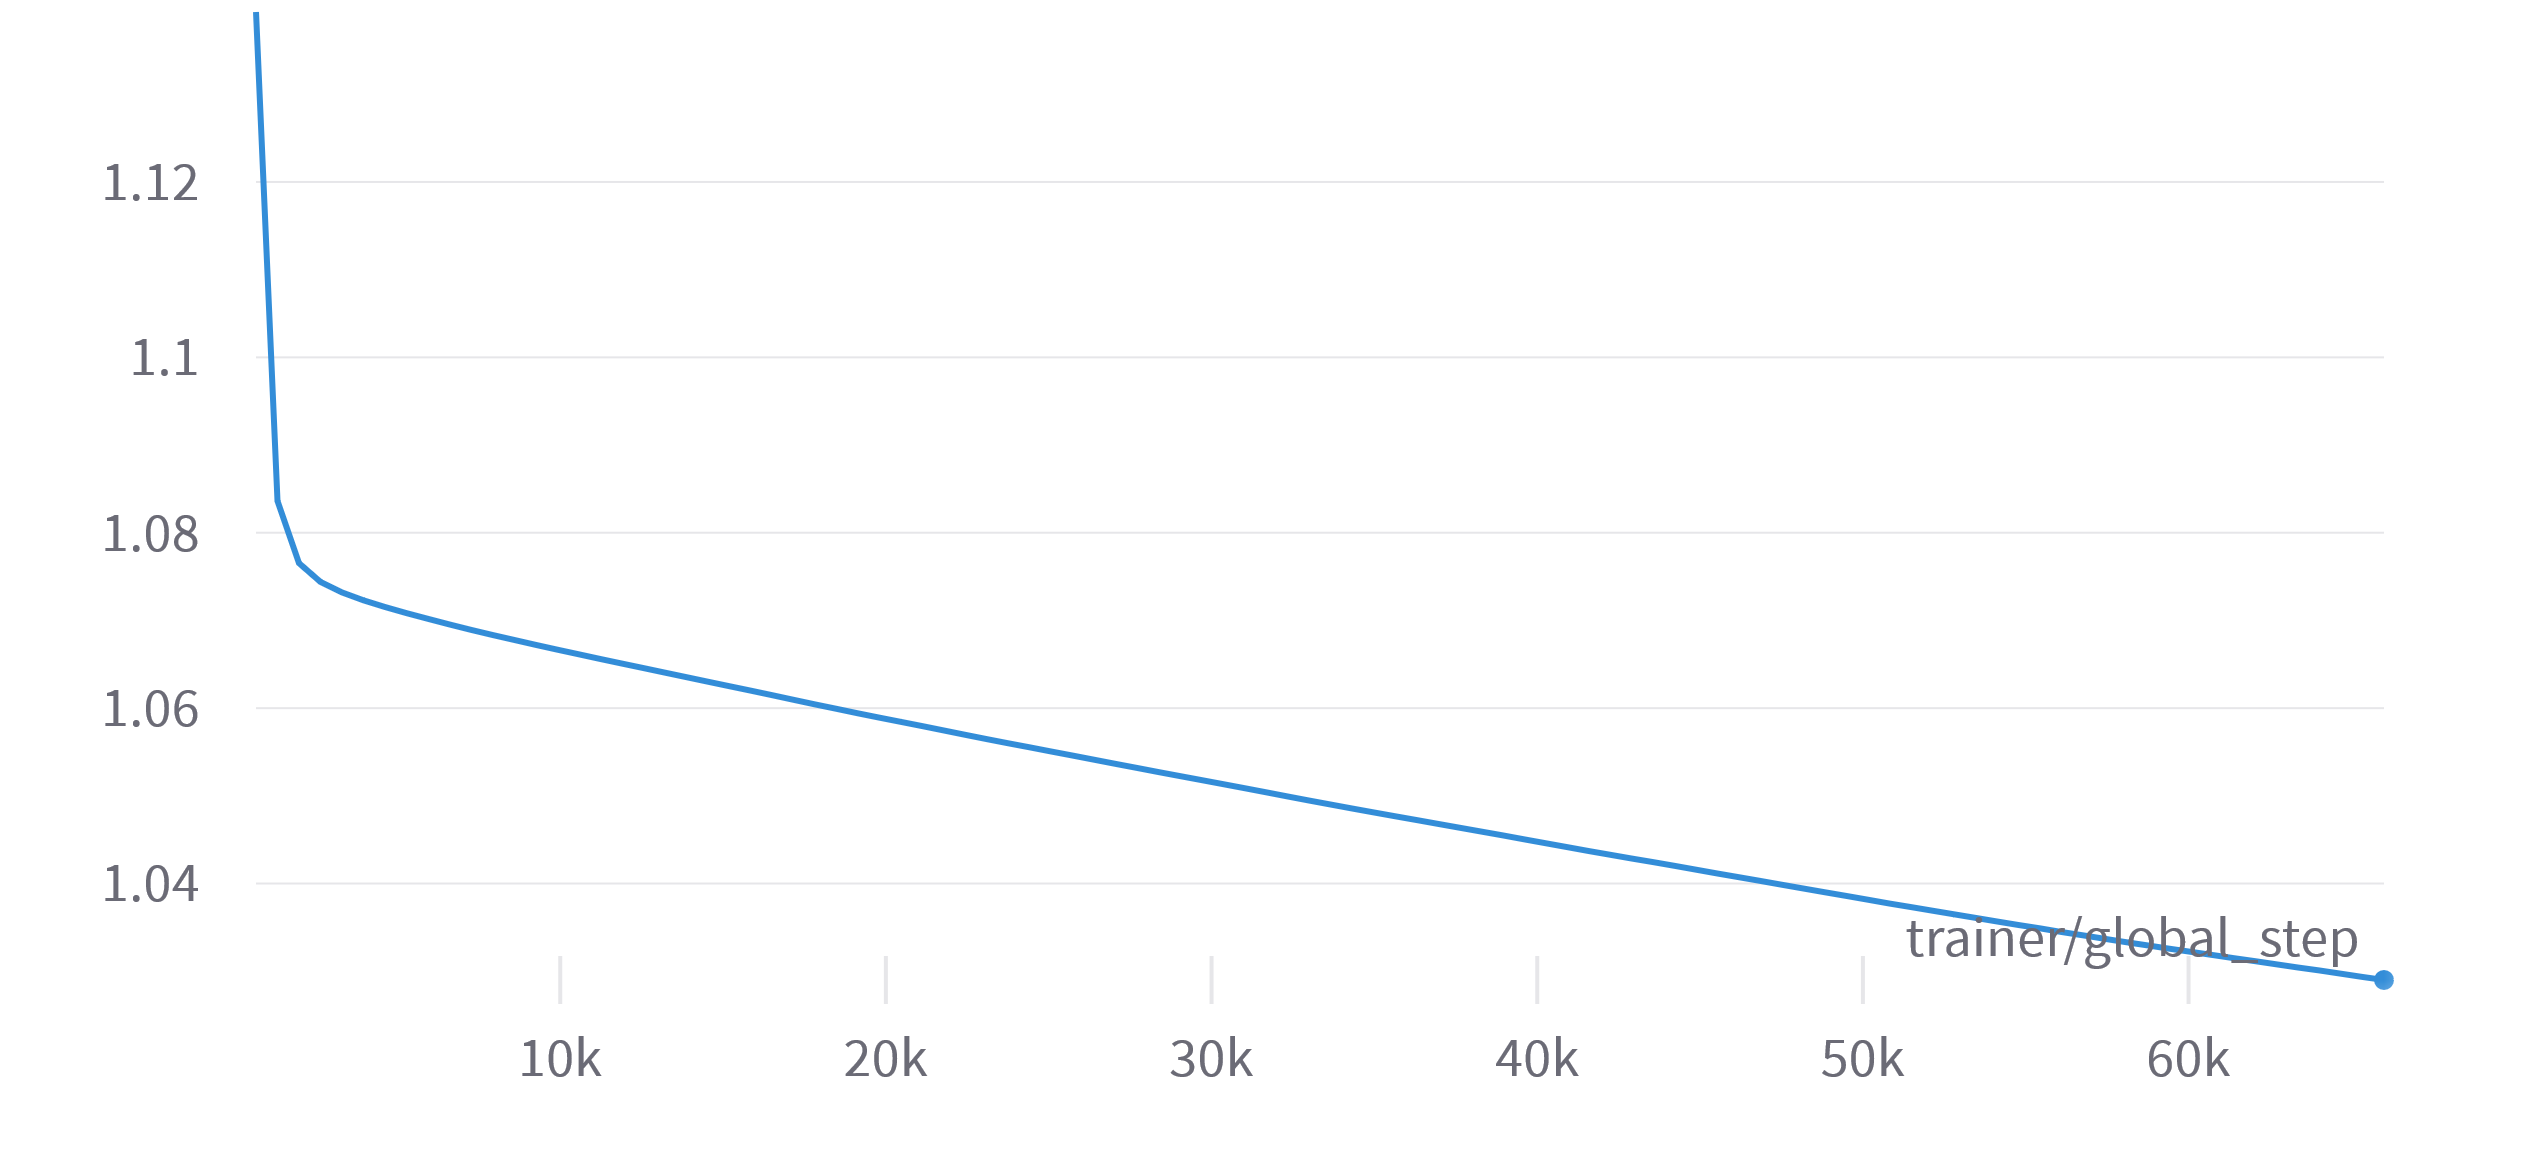
\includegraphics[width=\textwidth,height=\textheight,keepaspectratio]{figures/Learning Curve Example.png}
\end{frame}
\begin{frame}[fragile]{Learning Curve}
    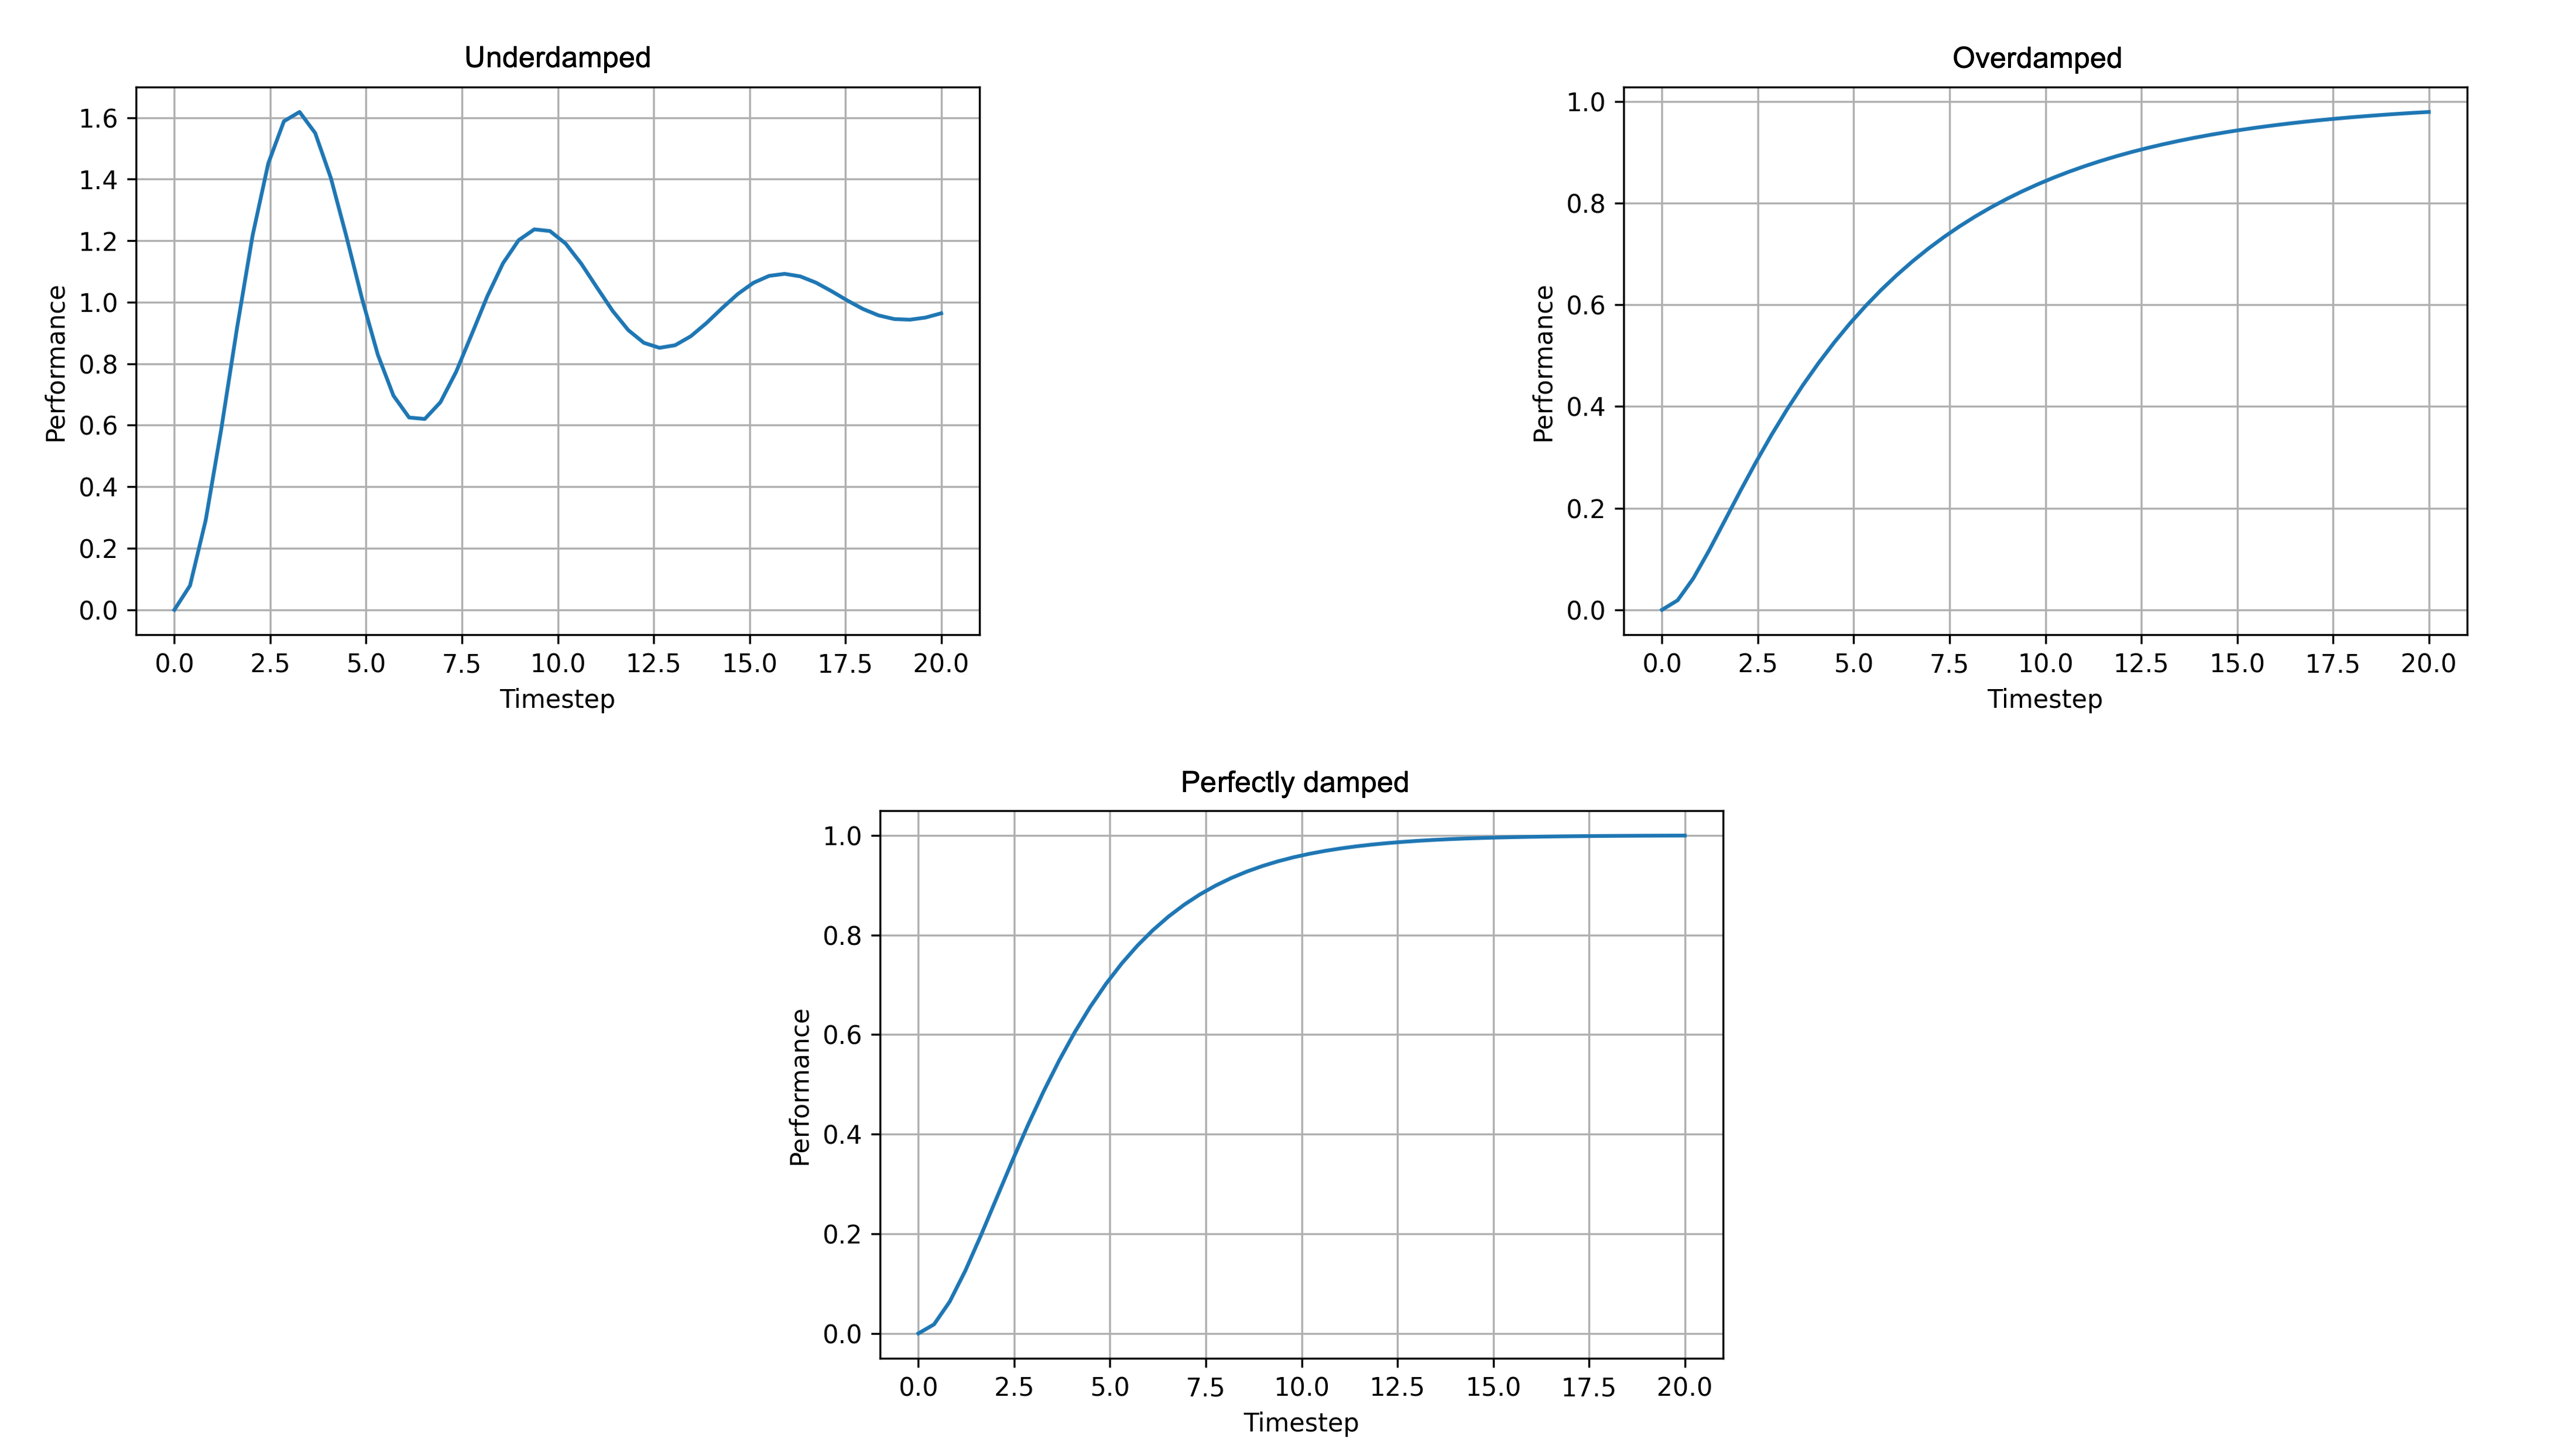
\includegraphics[width=\textwidth,height=\textheight,keepaspectratio]{figures/Dampness.png}
\end{frame}

\begin{frame}[fragile]{PyTorch}
    \textbf{PyTorch} is
    \begin{itemize}
        \item an open source Deep Learning library based on the Torch library, primarily developed by Facebook's AI Research lab.
        \item built upon an optimized C++ and CUDA code base that allows high throughput matrix operations on both the CPU and GPU.
    \end{itemize}
    \textbf{PyTorch}'s Python binding provides two high-level features:
    \begin{itemize}
        \item Tensor computation (like NumPy) with strong GPU acceleration
        \item Deep Neural Networks built on a tape-based autograd system and a dynamic computation graph
    \end{itemize}
\end{frame}
\begin{frame}[fragile]{GPU acceleration}
    Unlike traditional Machine Learning models, where parameters are usually optimized in a one-shot fashion, Deep Learning models' parameters are optimized iteratively, partially because of the training data volume and the models' structure. As a result, most computations in Deep Learning consisted of small matrix operations.\\
    Generally, CPUs are designed to be as versatile as possible, which means most CPUs are designed to accommodate large computations as fast as possible. In contrast, GPUs which handle screen displays are designed with one primary purpose: to do 3D geometry calculations as quickly as possible. As a result, most GPUs have significantly higher core counts than CPUs in the same era.\\
    \begin{center}
        \begin{tabular}{| c | c | c |}
            \hline
            \textbf{Device} & \textbf{Core Count} \\
            \hline
            AMD EPYC 9654 & 96 \\
            RTX 4090 & 16384 \\
            \hline
        \end{tabular}
    \end{center}
\end{frame}

\begin{frame}[fragile]{Tensor}
    \href{https://pytorch.org/docs/stable/tensors.html#torch.Tensor}{\textbf{torch.Tensor}} represent the main data structure for N-Dimensional tensors in PyTorch. Everything from parameters in the model to input data is stored in \textbf{torch.Tensor}. Although there are several operations to create  \textbf{torch.Tensor}, two of the most popular are:
    \begin{itemize}
        \item \href{https://pytorch.org/docs/stable/generated/torch.tensor.html}{\textbf{torch.tensor}}: Create a new tensor from an array-like data object. The tensor holds no autograd history.
        \item \href{https://pytorch.org/docs/stable/generated/torch.from_numpy.html}{\textbf{torch.from\_numpy}}: Create a new tensor from a NumPy array which shares the same memory. Changes to the tensor will be reflected in the NumPy array and vice versa.
        \item Aside from above, \textbf{torch.Tensor} also supports a NumPy-like interface in creating tensors such as:
        \begin{itemize}
            \item \href{https://pytorch.org/docs/stable/generated/torch.zeros.html}{\textbf{torch.zeros}}/\href{https://pytorch.org/docs/stable/generated/torch.ones.html}{\textbf{torch.ones}}
            \item \href{https://pytorch.org/docs/stable/generated/torch.arange.html}{\textbf{torch.arange}}
            \item \href{https://pytorch.org/docs/stable/generated/torch.rand.html}{\textbf{torch.rand}}
        \end{itemize}
    \end{itemize}
\end{frame}

\begin{frame}[fragile]{Module}
    \href{https://pytorch.org/docs/stable/nn.html}{\textbf{torch.nn}} provides basic building blocks for building a Deep Neural Network model. Aside from base classes for model containers, \textbf{torch.nn} also contain a generic implementation of popular layers such as RNN or Convolution.
    % There are two ways of defining a model in PyTorch:
    % \begin{itemize}
    %     \item \href{https://pytorch.org/docs/stable/generated/torch.nn.Module.html}{\textbf{torch.nn.Module}}
    %     \item \href{https://pytorch.org/docs/stable/generated/torch.nn.Sequential.html}{\textbf{torch.nn.Sequential}}
    % \end{itemize}
\end{frame}

\begin{frame}[fragile]{Datasets \& DataLoaders}
    \href{https://pytorch.org/docs/stable/generated/torch.nn.Module.html}{Dataset \& Data Loader} represent the main input pipeline with which the data is read from disk, preprocessed, and converted to a suitable type for a Deep Learning model.\\
    % In PyTorch, both "Dataset" and "Data Loader" are represented by these components:
    % \begin{itemize}
    %     \item \href{https://pytorch.org/docs/stable/data.html#torch.utils.data.Dataset}{\textbf{torch.utils.data.Dataset}}
    %     \item \href{https://pytorch.org/docs/stable/data.html#torch.utils.data.DataLoader}{\textbf{torch.utils.data.DataLoader}}
    % \end{itemize}
\end{frame}

\begin{frame}[fragile]{Mini-Batches?}
    Why do we need mini-batches? \\
    \begin{itemize}
        \item \textbf{Mini-batches} are used to reduce the memory footprint of the model and to speed up the training process.
        \item \textbf{Mini-batches} are also used to reduce the variance of the gradient estimate.
    \end{itemize}
    What batch size should we use? \\
    \begin{itemize}
        \item It depends
        \item Smaller batch sizes mean small gradients, which can slow down learning.
        \item Larger batch sizes increase the gradients' variances, making the model less accurate.
    \end{itemize}
\end{frame}

\begin{frame}[fragile]{Training Loop}
    A Training loop represents one of the most critical aspects of building Deep Learning models. The loop incorporates several significant elements, such as
    \begin{itemize}
        \item \textbf{Loss Function}: to calculate the loss
        \item \textbf{Optimizer}: to update the model parameters
    \end{itemize}
    Furthermore, events such as forward/backward passes, gradient descent, and parameter optimization happened in the training loop.
\end{frame}
\begin{frame}[fragile]{Loss Function \& Optimizer}
    \href{https://pytorch.org/docs/stable/nn.html#loss-functions}{\textbf{Loss Functions}} is another critical component in Deep Learning as it defines how output distribution and target distribution are compared. Generally, \textbf{Loss Functions} can be divided into two categories, depending on the data type:
    \begin{itemize}
        \item Discreet or Categorical: \textbf{Loss Functions} in this category are usually used to compare discreet or categorical distributions, most prevalent in classification tasks. Examples of this type of loss function are:
        % \begin{itemize}
        %     \item \href{https://pytorch.org/docs/stable/generated/torch.nn.CrossEntropyLoss.html}{\textbf{torch.nn.CrossEntropyLoss}}
        %     \item \href{https://pytorch.org/docs/stable/generated/torch.nn.BCEWithLogitsLoss.html}{\textbf{torch.nn.BCEWithLogitsLoss}}
        % \end{itemize}
        \item Continuous: \textbf{Loss Functions} in this category are primarily used in regression or encoding tasks as most distributions in these tasks are continuous. Examples of this type of loss function are:
        % \begin{itemize}
        %     \item \href{https://pytorch.org/docs/stable/generated/torch.nn.MSELoss.html#torch.nn.MSELoss}{\textbf{torch.nn.MSELoss}}
        %     \item \href{https://pytorch.org/docs/stable/generated/torch.nn.TripletMarginLoss.html}{\textbf{torch.nn.TripletMarginLoss}}
        % \end{itemize}
    \end{itemize}
    % In PyTorch, most loss functions are implemented with {torch.nn.Module} as a base class with a functional backend.
    {\textbf{Optimizers}} are another essential aspect of Deep Learning as they contain an update strategy for all the parameters.
\end{frame}
% \begin{frame}[fragile]{Optimizer}
%     \href{https://pytorch.org/docs/stable/optim.html}{\textbf{Optimizers}} are another essential aspect of Deep Learning as they contain an update strategy for all the parameters. In PyTorch, all \textbf{Optimizers} are implemented with {torch.nn.Module} as a base class with a functional backend.
%     % \begin{itemize}
%     %     \item \href{https://pytorch.org/docs/stable/generated/torch.optim.SGD.html}{\textbf{torch.optim.SGD}}: Implements stochastic gradient descent (optionally with momentum).
%     %     \item \href{https://pytorch.org/docs/stable/generated/torch.optim.Adam.html}{\textbf{torch.optim.Adam}}: Implements Adam algorithm.
%     %     \item \href{https://pytorch.org/docs/stable/generated/torch.optim.Adamax.html}{\textbf{torch.optim.Adamax}}: Implements Adamax algorithm.
%     %     \item \href{https://pytorch.org/docs/stable/generated/torch.optim.RMSprop.html}{\textbf{torch.optim.RMSprop}}: Implements RMSprop algorithm.
%     %     \item \href{https://pytorch.org/docs/stable/generated/torch.optim.SparseAdam.html}{\textbf{torch.optim.SparseAdam}}: Implements Adam algorithm for sparse tensors.
%     % \end{itemize}
% \end{frame}

\begin{frame}[fragile]{Training Loop}
    \begin{exampleblock}{}
        \begin{lstlisting}[language=Python]
loss_fn = LossFunction()
optimizer = Optimizer(model.parameters(), lr=0.01)
for t in range(epochs):
for x, y in train_dataloader:
    y_pred = model(x)
    # Compute loss
    loss = loss_fn(y_pred, y)
    # Clear previous gradients
    optimizer.zero_grad()
    # Compute gradients
    loss.backward()
    # Update parameters
    optimizer.step()
        \end{lstlisting}
    \end{exampleblock}
\end{frame}

\begin{frame}[fragile]{Generic Modules in PyTorch}
    Aside from {Module}, and {Loss Functions}, {torch.nn} also contains generic implementations of popular layers such as:
    \begin{itemize}
        \item \href{https://pytorch.org/docs/stable/nn.html#linear-layers}{\textbf{Linear Layers}}
        \item \href{https://pytorch.org/docs/stable/nn.html#convolution-layers}{\textbf{Convolutional Layers}}
        \item \href{https://pytorch.org/docs/stable/nn.html#recurrent-layers}{\textbf{Recurrent Layers}}
        \item \href{https://pytorch.org/docs/stable/nn.html#normalization-layers}{\textbf{Normalization Layers}}
        \item \href{https://pytorch.org/docs/stable/nn.html#non-linear-activations-weighted-sum-nonlinearity}{\textbf{Activation Layers}}
    \end{itemize}
\end{frame}

\begin{frame}[fragile]{Linear Layers}
    \href{https://pytorch.org/docs/stable/nn.html#linear-layers}{\textbf{Linear Layers}} are the most basic layer in a neural network. They are used to transform the input data into a different space by multiplying the last dimension of the tensor, $H_{in}$, with a weight of size ($H_{in}$, $H_{out}$)
    \begin{center}
        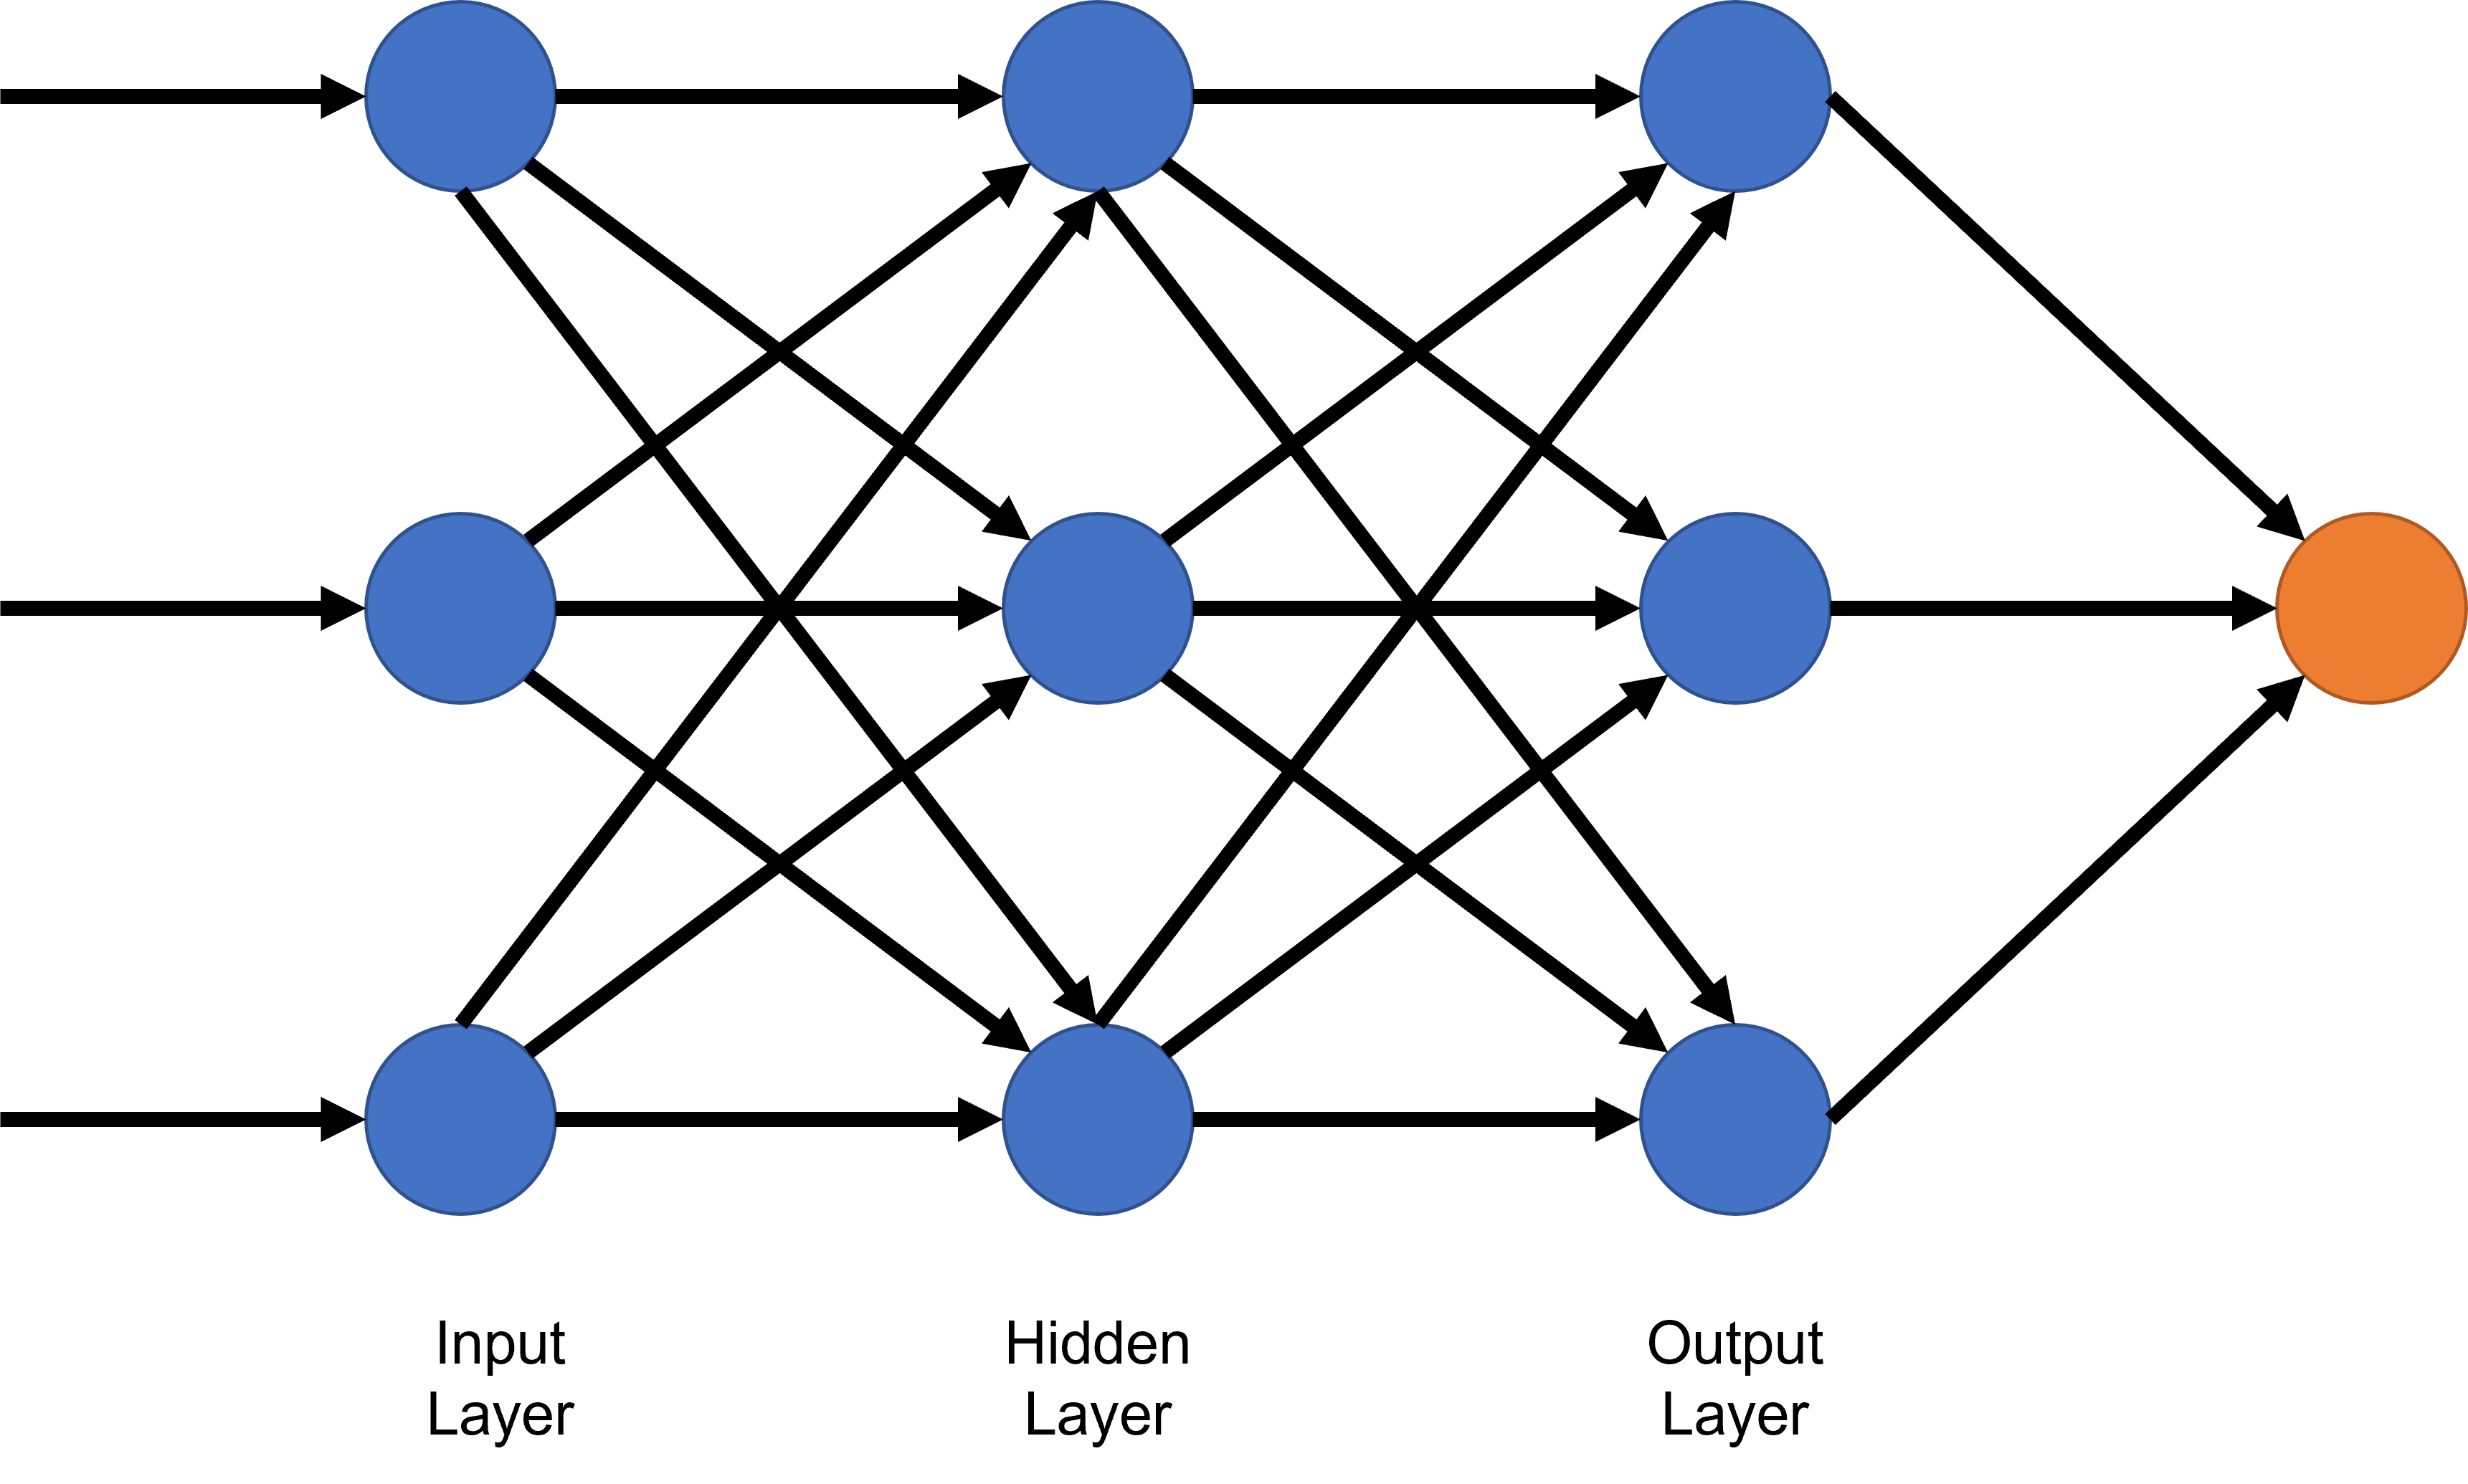
\includegraphics[width=\textwidth,height=0.7\textheight,keepaspectratio]{figures/SimpleNN.png}
    \end{center}
\end{frame}
\begin{frame}[fragile]{Linear Layers}
    In PyTorch, the {Linear} layer is implemented as:
    \begin{exampleblock}{}
        \begin{lstlisting}[language=Python]
class torch.nn.Linear(
in_features, out_features,
bias=True, device=None, dtype=None
)
        \end{lstlisting}
    \end{exampleblock}
\end{frame}

\begin{frame}[fragile]{Activation Layers}
    \href{https://pytorch.org/docs/stable/nn.html#non-linear-activations-weighted-sum-nonlinearity}{\textbf{Activation Layers}} \\
    \begin{itemize}
        \item Nonlinear Activation Layers represent one of the hallmarks of Deep Learning models. Adding nonlinearity adds more complexities to the model and allows the model to operate in nonlinear space where most real-life equations reside.
        % \item The most common activation layers are:
        % \begin{itemize}
        %     \item \href{https://pytorch.org/docs/stable/generated/torch.nn.ReLU.html}{\textbf{torch.nn.ReLU}} applies the rectified linear unit function element-wise that sets the minimum value to 0: $f(x) = max(0, x)$
        %     \item \href{https://pytorch.org/docs/stable/generated/torch.nn.Sigmoid.html}{\textbf{torch.nn.Sigmoid}} applies the sigmoid function element-wise, which maps the value to the range of [0, 1]: $f(x) = \frac{1}{1 + e^{-x}}$
        %     \item \href{https://pytorch.org/docs/stable/generated/torch.nn.Tanh.html}{\textbf{torch.nn.Tanh}} applies the hyperbolic tangent function element-wise, which maps the value to the range of [-1, 1]: $f(x) = \frac{e^x - e^{-x}}{e^x + e^{-x}}$
        %     \item \href{https://pytorch.org/docs/stable/generated/torch.nn.Softmax.html}{\textbf{torch.nn.Softmax}} applies the softmax function element-wise, which maps the value to the range of [0, 1] and normalizes the output to sum to 1: $f(x) = \frac{e^x}{\sum_{i=1}^{n} e^x}$
        % \end{itemize}
    \end{itemize}
\end{frame}

\begin{frame}[fragile]{Convolution Layers}
    \href{https://pytorch.org/docs/stable/nn.html#convolution-layers}{\textbf{Convolution Layers}} are among the most popular layers in a vision neural network. The layer used convolutional filters to extract repeating relevant local features from the data.
    \begin{figure}
        \begin{overprint}
            \onslide<1>\centering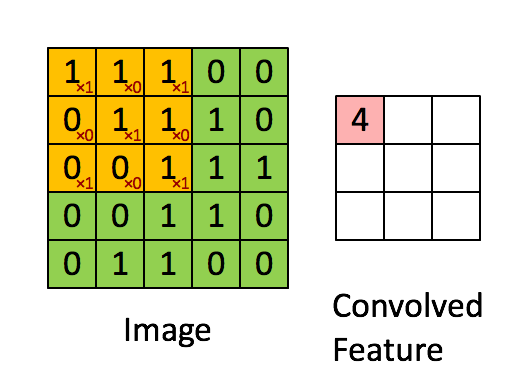
\includegraphics[width=.7\textwidth,height=\textheight,keepaspectratio]{figures/Convolution/Convolution-0.png}
            \onslide<2>\centering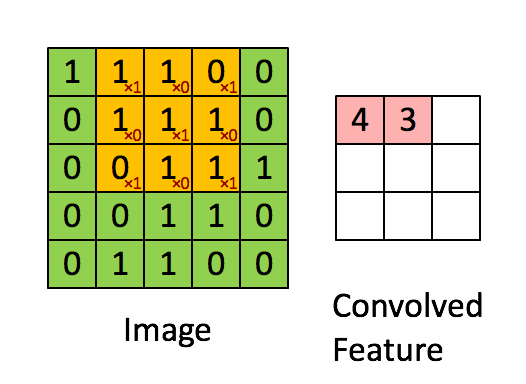
\includegraphics[width=.7\textwidth,height=\textheight,keepaspectratio]{figures/Convolution/Convolution-1.png}
            \onslide<3>\centering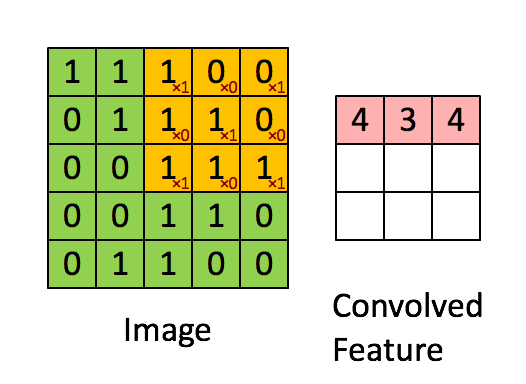
\includegraphics[width=.7\textwidth,height=\textheight,keepaspectratio]{figures/Convolution/Convolution-2.png}
            \onslide<4>\centering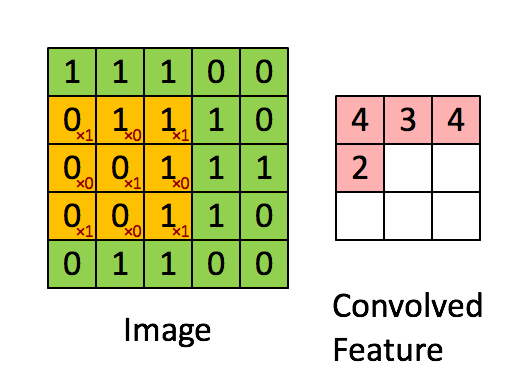
\includegraphics[width=.7\textwidth,height=\textheight,keepaspectratio]{figures/Convolution/Convolution-3.png}
            \onslide<5>\centering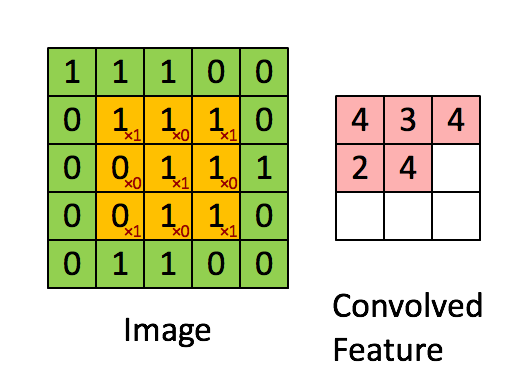
\includegraphics[width=.7\textwidth,height=\textheight,keepaspectratio]{figures/Convolution/Convolution-4.png}
            \onslide<6>\centering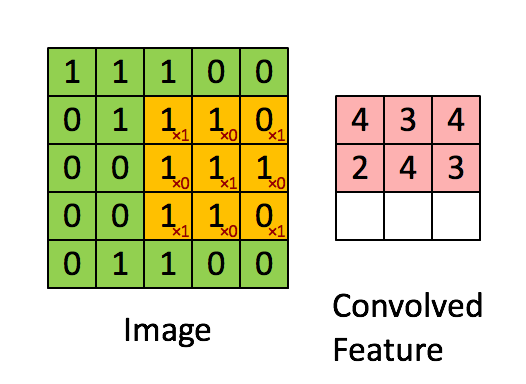
\includegraphics[width=.7\textwidth,height=\textheight,keepaspectratio]{figures/Convolution/Convolution-5.png}
            \onslide<7>\centering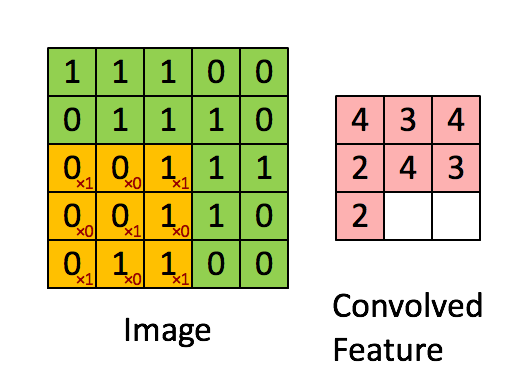
\includegraphics[width=.7\textwidth,height=\textheight,keepaspectratio]{figures/Convolution/Convolution-6.png}
            \onslide<8>\centering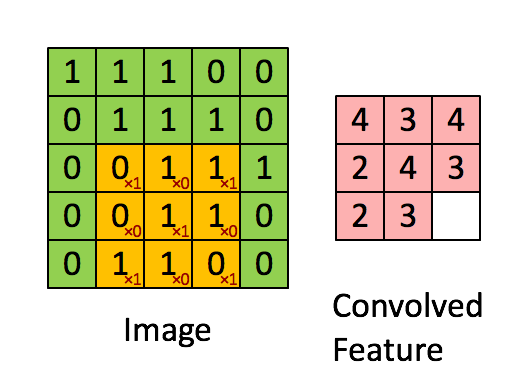
\includegraphics[width=.7\textwidth,height=\textheight,keepaspectratio]{figures/Convolution/Convolution-7.png}
            \onslide<9->\centering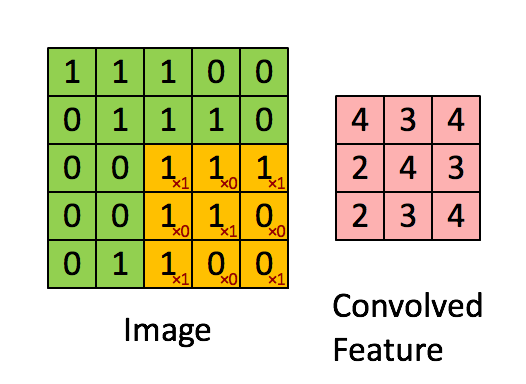
\includegraphics[width=.7\textwidth,height=\textheight,keepaspectratio]{figures/Convolution/Convolution-8.png}
        \end{overprint}
    \end{figure}
\end{frame}
\begin{frame}[fragile]{Convolution Layers}
    Torch contains several implementations of Convolution Layers. The most common, \href{https://pytorch.org/docs/stable/generated/torch.nn.Conv2d.html}{\textbf{torch.nn.Conv2d}}, is implemented as:
    \begin{exampleblock}{}
        \begin{lstlisting}[language=Python]
class torch.nn.Conv2d(
in_channels, out_channels,
kernel_size, stride=1, padding=0,
dilation=1, groups=1, bias=True,
padding_mode='zeros', device=None,
dtype=None
)
        \end{lstlisting}
    \end{exampleblock}
\end{frame}

\begin{frame}[fragile]{Recurrent Layers}
    \href{https://pytorch.org/docs/stable/nn.html#recurrent-layers}{\textbf{Recurrent Layers}} are layers in a neural network that process sequential data. They used recurrent signals to model temporal dependency in the data.
    \begin{figure}
        \begin{overprint}
            \onslide<1>\centering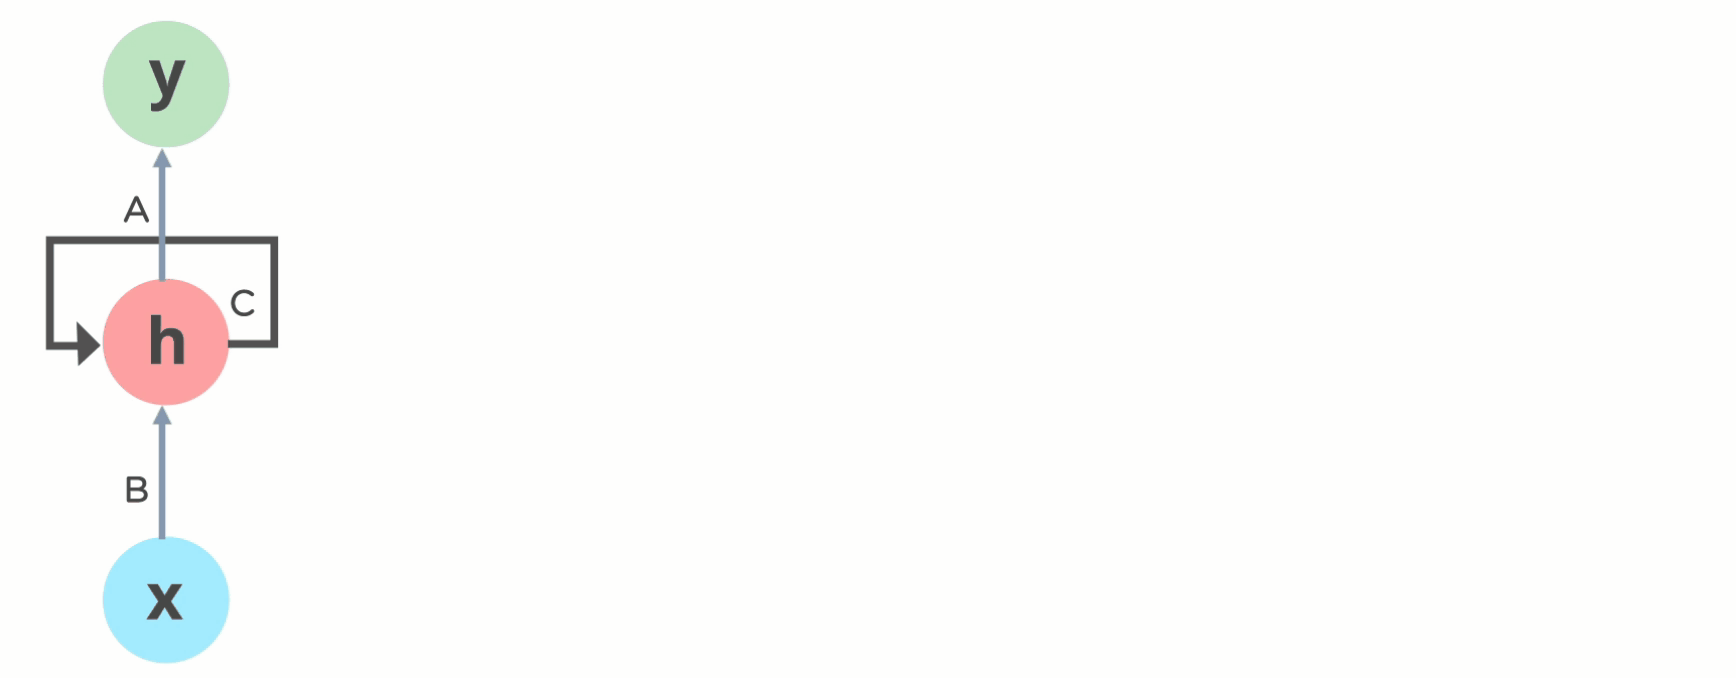
\includegraphics[width=\textwidth,height=\textheight,keepaspectratio]{figures/RNN/frame_apngframe06.png}
            \onslide<2->\centering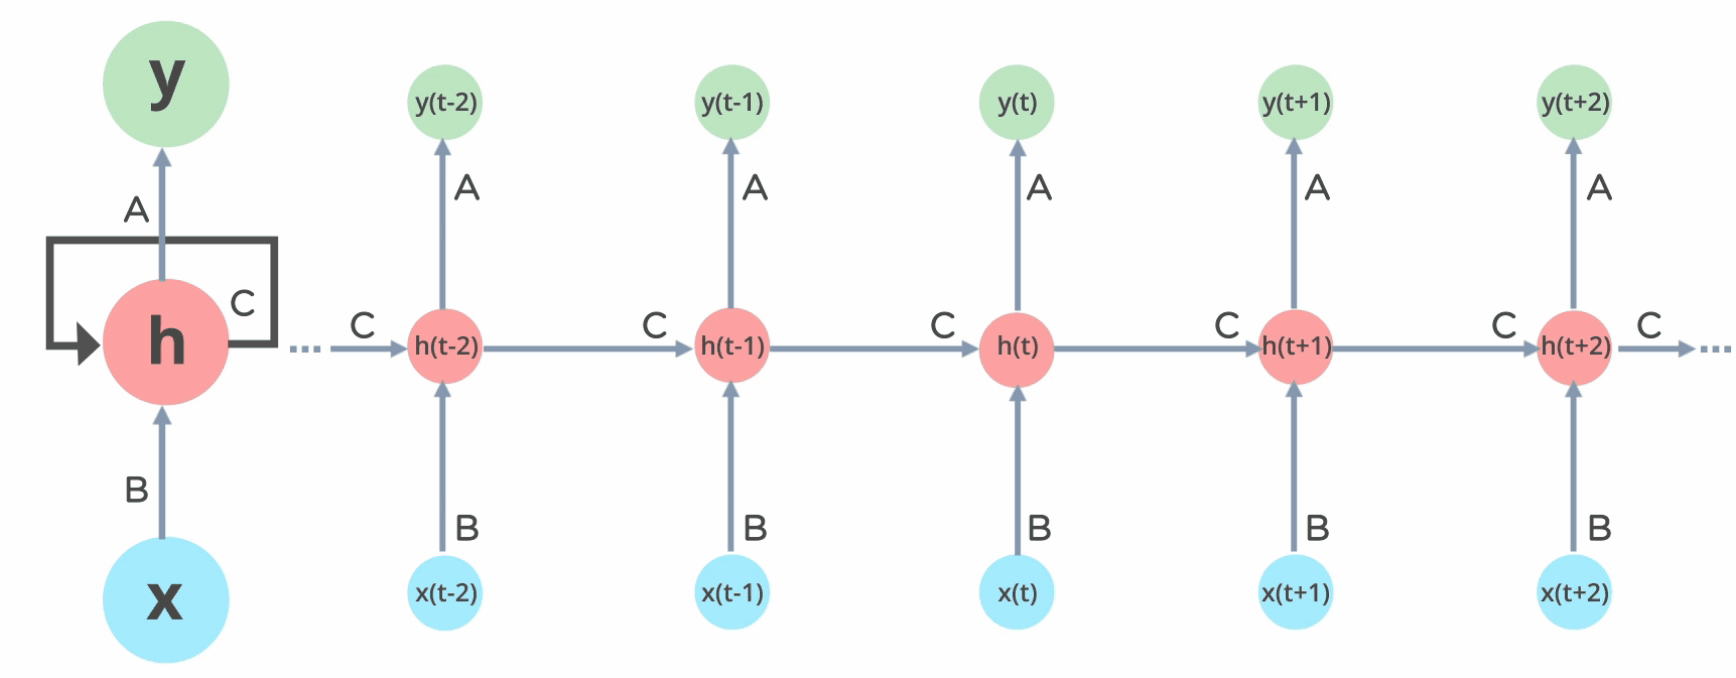
\includegraphics[width=\textwidth,height=\textheight,keepaspectratio]{figures/RNN/frame_apngframe16.png}
        \end{overprint}
    \end{figure}
\end{frame}
\begin{frame}[fragile]{Recurrent Layers}
    There are several Recurrent Layers implemented in PyTorch, i.e. \href{https://pytorch.org/docs/stable/generated/torch.nn.RNN.html}{\textbf{Vanilla RNN}}, \href{https://pytorch.org/docs/stable/generated/torch.nn.GRU.html}{\textbf{GRU}}, and \href{https://pytorch.org/docs/stable/generated/torch.nn.LSTM.html}{\textbf{LSTM}}. However, most share the standard constructor as follows:
    \begin{exampleblock}{}
        \begin{lstlisting}[language=Python]
class torch.nn.LSTM(
input_size, hidden_size,
num_layers=1, bias=True,
batch_first=False, dropout=0,
bidirectional=False, device=None,
dtype=None
)
        \end{lstlisting}
    \end{exampleblock}
    % \begin{alertblock}{Caution}
    %     Although most layers in PyTorch return the product of the layer when called, recurrent layers return a tuple of (output, final hidden states).
    % \end{alertblock}
\end{frame}

\begin{frame}[fragile]{Normalization Layers}
    In 2015, \href{https://arxiv.org/abs/1502.03167}{\textbf{Ioffe and Szegedy}} discovered that even though Deep Neural Networks can approximate data distribution, the distributional shift within each layer can significantly impact performance and training time. Thus were born the \href{https://pytorch.org/docs/stable/nn.html#normalization-layers}{\textbf{Normalization Layers}}, which normalize each layer input to a standard Gaussian distribution. This method significantly increases model performance and decreases training time.
\end{frame}
\begin{frame}[fragile]{Normalization Layers}
    \centering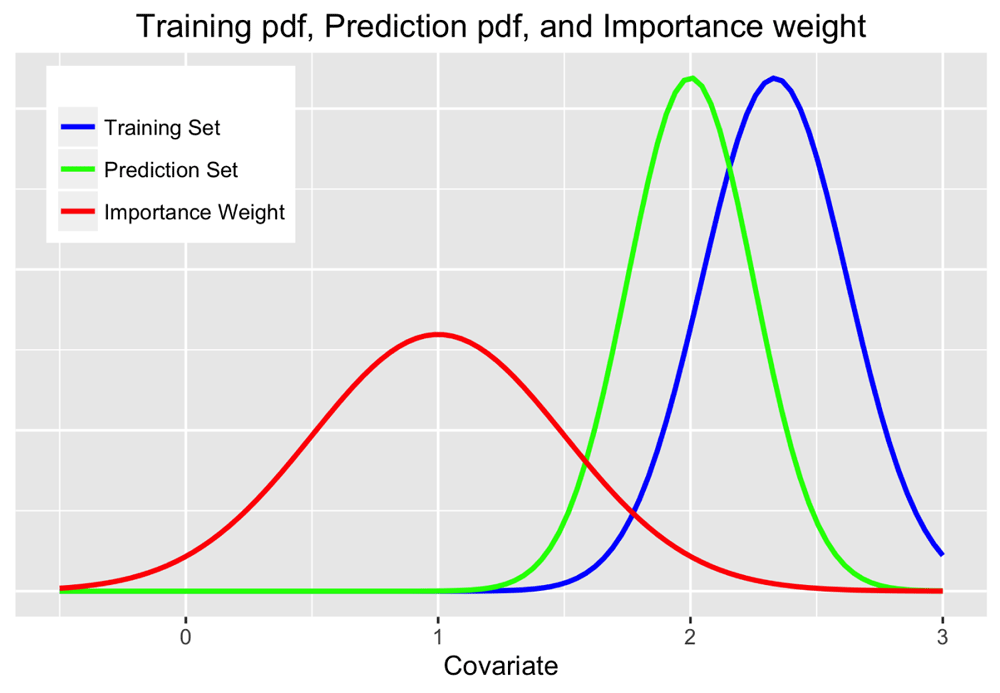
\includegraphics[width=\textwidth,height=\textheight,keepaspectratio]{figures/Covariance.png}
\end{frame}
\begin{frame}[fragile]{Normalization Layers}
    In PyTorch, there are implementations of multiple Normalization layers such as \href{https://arxiv.org/abs/1502.03167}{\textbf{Batch Normalization}}, \href{https://arxiv.org/abs/1607.06450}{\textbf{Layer Normalization}}, \href{https://arxiv.org/abs/1803.08494}{\textbf{Group Normalization}}, and \href{https://arxiv.org/abs/1701.02096}{\textbf{Instance Normalization}}. The most common, \href{https://pytorch.org/docs/stable/generated/torch.nn.BatchNorm2d.html}{\textbf{BatchNorm2d}}, is implemented as:
    \begin{exampleblock}{}
        \begin{lstlisting}[language=Python]
class torch.nn.BatchNorm2d(
num_features, eps=1e-05,
momentum=0.1, affine=True,
track_running_stats=True,
device=None, dtype=None
)
        \end{lstlisting}
    \end{exampleblock}
\end{frame}

\begin{frame}[fragile]{Transformers}
    \begin{center}
        \includegraphics[width=\textwidth,height=0.9\textheight,keepaspectratio]{figures/electrical_transformer.png}
    \end{center}
\end{frame}

\begin{frame}[fragile]{Transformers}
    \begin{center}
        \includegraphics[width=\textwidth,height=0.8\textheight,keepaspectratio]{figures/PrimeRenderROTB.png}
    \end{center}
\end{frame}
\begin{frame}[fragile]{Transformers}
    \begin{center}
        \includegraphics[width=\textwidth,height=0.8\textheight,keepaspectratio]{figures/Transformer-Model.png}
    \end{center}
\end{frame}

\begin{frame}[fragile]{Transformers}
    \begin{columns}[T]
        \begin{column}{.48\textwidth}
            \begin{center}
                \includegraphics[width=\textwidth,height=0.8\textheight,keepaspectratio]{figures/Transformer-Model.png}
            \end{center}
        \end{column}%
        \hfill%
        \begin{column}{.48\textwidth}
            \begin{itemize}
                \item First proposed in 2017 paper, \href{https://arxiv.org/abs/1706.03762}{"\textbf{Attention Is All You Need}"}, by Ashish Vaswani et al., Transformers have become a fundamental building block for various applications, including language translation, text summarization, image recognition.
            \end{itemize}
        \end{column}%
    \end{columns}
\end{frame}
\begin{frame}[fragile]{Transformers}
    \begin{columns}[T]
        \begin{column}{.48\textwidth}
            \begin{center}
                \includegraphics[width=\textwidth,height=0.8\textheight,keepaspectratio]{figures/Transformer-Model.png}
            \end{center}
        \end{column}%
        \hfill%
        \begin{column}{.48\textwidth}
            \begin{itemize}
                \item The key innovation lies in the Scaled-Dot product Attention that allows each layer to focus on different parts of the input sequence, resulting in more effective temporal modelling.
                \item Transformers applications such as BERT or GPT have achieved state-of-the-art performance on various language understanding tasks.
            \end{itemize}
        \end{column}%
    \end{columns}
\end{frame}
% \begin{frame}[fragile]{Transformers}
%     \begin{columns}[T]
%         \begin{column}{.48\textwidth}
%             \begin{center}
%                 \includegraphics[width=\textwidth,height=0.8\textheight,keepaspectratio]{Scaled-Dot_product.png}
%             \end{center}
%         \end{column}
%         \hfill
%         \begin{column}{.48\textwidth}
%             \begin{center}
%                 \includegraphics[width=\textwidth,height=0.8\textheight,keepaspectratio]{Attention-matrix-visualization-a-weights-in-BERT-Encoding-Unit-Entity-BERT-b.png}
%             \end{center}
%         \end{column}
%     \end{columns}
% \end{frame}
\section{The End}
\end{document}